
\documentclass[11pt]{acmeArticle}
\usepackage{amssymb,amsthm,mathrsfs,graphicx, bm}
\usepackage{natbib}
\usepackage{subfigure}
\usepackage{titlesec}
\usepackage{geometry}
\usepackage{fancyhdr}
\usepackage{newtxtext,newtxmath}
\usepackage{hyperref}

\usepackage{amsmath}
\usepackage{color}
\usepackage{amsfonts}
%\DeclareMathOperator*{\Aoperator}{ \mathlarger{\mathlarger{\mathlarger{\boldsymbol{\mathsf{A}}}}} }
\DeclareMathOperator*{\aoperator}{ \text{\huge${\mathsf{A}}$}}
\pagenumbering{arabic}


%Packages for Matlab2TikZ
\usepackage{pgfplots}
\pgfplotsset{compat=newest}
\usetikzlibrary{plotmarks}
\usetikzlibrary{arrows.meta}
\usepgfplotslibrary{patchplots}
\usepackage{grffile}


\setlength{\parindent}{0pt}
\setlength{\parskip}{5pt plus 2pt minus 1 pt}

\numberwithin{equation}{section}
%\topmargin  -25mm
%\evensidemargin 0mm
%\oddsidemargin  0mm
%\textwidth  160mm
%\textheight 267mm
\renewcommand{\baselinestretch}{1.0}
\frenchspacing
\sloppy
\titlespacing{\section}{0pt}{\parskip}{0.01\parskip}
\renewcommand{\headrulewidth}{0pt}
%%%%%%%%%%%%%%%%%%%%%%%%%%%%%%%%%%%%%%%%%%%%%%%%%%%%%%%%%%%%%%%%%%%%%%%


\begin {document}
%\setcounter{page}{3}

\vspace*{-1mm}
\thispagestyle{fancy} 
%\fancyhead[R]{{}
\rhead{{\footnotesize
		\it September 2018, Glasgow\\} }
\cfoot{}

%\pagestyle{empty}

\begin{center}
	
	{\fontsize{14}{20}\bf Numerical investigation into fracture risk of equine metacarpal bone following adaptation}\end{center}

%\restoregeometry

\begin{center}
	\textbf{Karol Lewandowski }\\
	\textbf{{\L}ukasz Kaczmarczyk, Ignatios Athanasiadis, John F. Marshall, Chris J. Pearce }\\
	{School of Engineering} \\
	{University of Glasgow}
\end{center}
%
{\clearpage}

\begin{center}
	\textbf{ABSTRACT}\\[1mm]
\end{center}
%


{\small 
	Fractures of the metacarpal condyle are a common orthopaedic injury in Thoroughbred racehorses.  
	A large proportion of injuries occur in the absence of a specific traumatic event and show typical characteristics of stress fractures. 
	The purpose of this work is to develop a combined remodelling and fracture finite element based framework allowing for integrated simulation of an~equine 3rd metacarpal remodelling under specific exercise regime (boundary conditions), followed by the evaluation of its fracture release energy. 
	The proposed approach can improve the understanding of the correlation between high exercise intensity, bone adaptation and fracture 
	risk, ultimately improving the welfare of the racehorse. 
	The remodelling analysis is based on a phenomenological model of the macroscopic behaviour of bone based on thermodynamics of open 
	systems previously presented in the literature. 
	Assessment of fracture propensity is conducted by evaluating strain release energy rate within the context of configurational mechanics. 
	All analyses are performed using unstructured tetrahedral meshes. 
	Material mapping between remodelling analysis mesh and fracture analysis mesh is obtained through Moving Least Squares approximation. 
	Hierarchical basis functions of arbitrary polynomial order are adopted to increase the order of approximation, to achieve high 
	accuracy results with relatively coarse meshes and to take advantage of efficient multigrid solvers.
	Extension of Quarter Point Elements tailored for hierarchical basis functions is proposed to solve the stress singularity at the 
	crack tip.
	The implemented framework provides a robust and energy consistent method for quantifying the influence of bone adaptation on the
	 fracture propensity.
	Performance, verification, convergence and validation of the presented method are demonstrated by numerical examples.
	The promising results of this study offer a~novel framework to simulate changes in the bone structure in response to exercise and 
	quantify the fracture propensity.
	 
	%Bone is able to adapt to changes in its mechanical environment. Studies of the Thoroughbred racehorse show modification of the geometric properties of the third metacarpal bone in response to training. These modifications are associated with reduced bone strains. Intense training before the adaptive response is completed and bone strain reduced increases the risk of fatigue damage. Bone adaptation in response to different loads is known to increase the resistance to fracture. The development of computational models to describe bone behavior has gained tremendous importance over the last decade. In particular, computational modelling for bone growth and resorption processes followed by fracture analysis can be a useful tool to determine crack propensity. Therefore,, this study aims to develop an efficient framework which will help to understand the relationship between exercise loading, bone density and ultimately fracture risk. This case study highlights the development of subject-specific FE analyses to simulate exercise loading on equine bone and subsequently quantify changes in the fracture propensity in open source code - MoFEM.
	
\textbf{\textit{Key Words:}} {\it finite element analysis, bone remodelling, fracture, 3rd metacarpal, moving least squares, configurational mechanics, heterogeneity}}
%
\\
\newpage
\clearpage
\pagenumbering{arabic}



\textcolor{red}{All the figures are still in draft mode.}
\section{Introduction}
In the UK, approximately 60\% of horse fatalities at racecourses are associated with a fracture, with the distal limb the most commonly affected site \citep{parkin2004horse}.
Most of these fractures occur due to the accumulation of tissue fatigue, as a result of repetitive loading~\citep{Parkin2005}, rather than a specific traumatic event. 
Racehorses experience extreme bone remodelling, with intense exercise and excessive loading of the metacarpal bones resulting in maladaptation. Remodelling is the on-going complex biological process of replacing old bone tissue by new bone and thus repairing the fatigue damage~\citep{hughes2017role}.
The bone repair is overwhelmed by load-induced bone densification that also increases brittleness~\citep{loughridge2017qualitative}.

The location of 3rd metacarpal fractures is remarkably consistent across a large number of racehorses,  crack initiation presenting from 
the lateral para-sagittal groove of the distal condyle of the leading forelimb~\citep{jacklin2012frequency, parkin2006analysis}.
Despite considerable research in the field, including applying diagnostic methods such as radiography 
\citep{bogers2016quantitative, crijns2014intramodality, loughridge2017qualitative}, magnetic resonance imaging 
\citep{tranquille2017MRI} and biomarkers~\citep{mcilwraith2005use}, it still remains a challenge to accurately predict the fracture risk 
and prevent this type of significant injury.
This paper focuses on the use of computational tools to quantify bone adaptation and resistance to fracture, thereby providing the basis for a 
viable and robust solution.
The use of computational tools to describe bone behaviour has gained a tremendous importance over the last decade. 
In particular, the Finite Element Method (FEM) has been used to improve understanding of the fracture behaviour of bones and the relationships between load conditions and bone architecture~\citep{podshivalov2014road, poelert2013patient}. However, there are only a few example of the numerical analysis of both bone remodelling and fracture, e.g.~\citep{hambli2013integrated}.

The novelty of this paper is a computational framework based on FEM to predict bone density profiles 
(bone adaptation) due to exercise and subsequently quantify fracture resistance of 
adapted bones using linear elastic fracture mechanics. 
A schematic of the procedure is presented in Figure~\ref{fig:framework}.
%(The aim for this study is the establishment and implementation of FEM based framework suitable for clinical practice that will help to simulate density evolution, quantify current and future fracture risk based on CT scanning data derived from horses in training.) 
%Bone adaptation process, within the developed framework, is incorporated by using computational algorithm in open system thermodynamics 
%\citep{Kuhl2003a}.

This article is structured as follows. The mathematical framework for bone remodelling is briefly presented in Section~\ref{sec:bone_remodel}.
Section~\ref{sec:dens_mapping} describes a novel approach to assign heterogeneous mechanical bone properties, derived from CT scans,
to the finite element model by means of the Moving Least Squares (MLS) method.
Thereafter, Section~\ref{sec:release_energy} presents an extension of a recently established approach 
for evolving crack propagation in the context of configurational mechanics. The method is utilised to calculate the energy release rate of bones under quasi-static loading during different stages of adaptation. 
Section~\ref{sec:numerical_examples} brings together all the developments of the framework in the form of numerical examples. 
Finally, a brief summary of the work is presented in Section~\ref{sec:discussion} and areas for further research are identified.

\begin{figure}[h]
	\centering
	   \begin{tikzpicture}
		\node at (0,4) {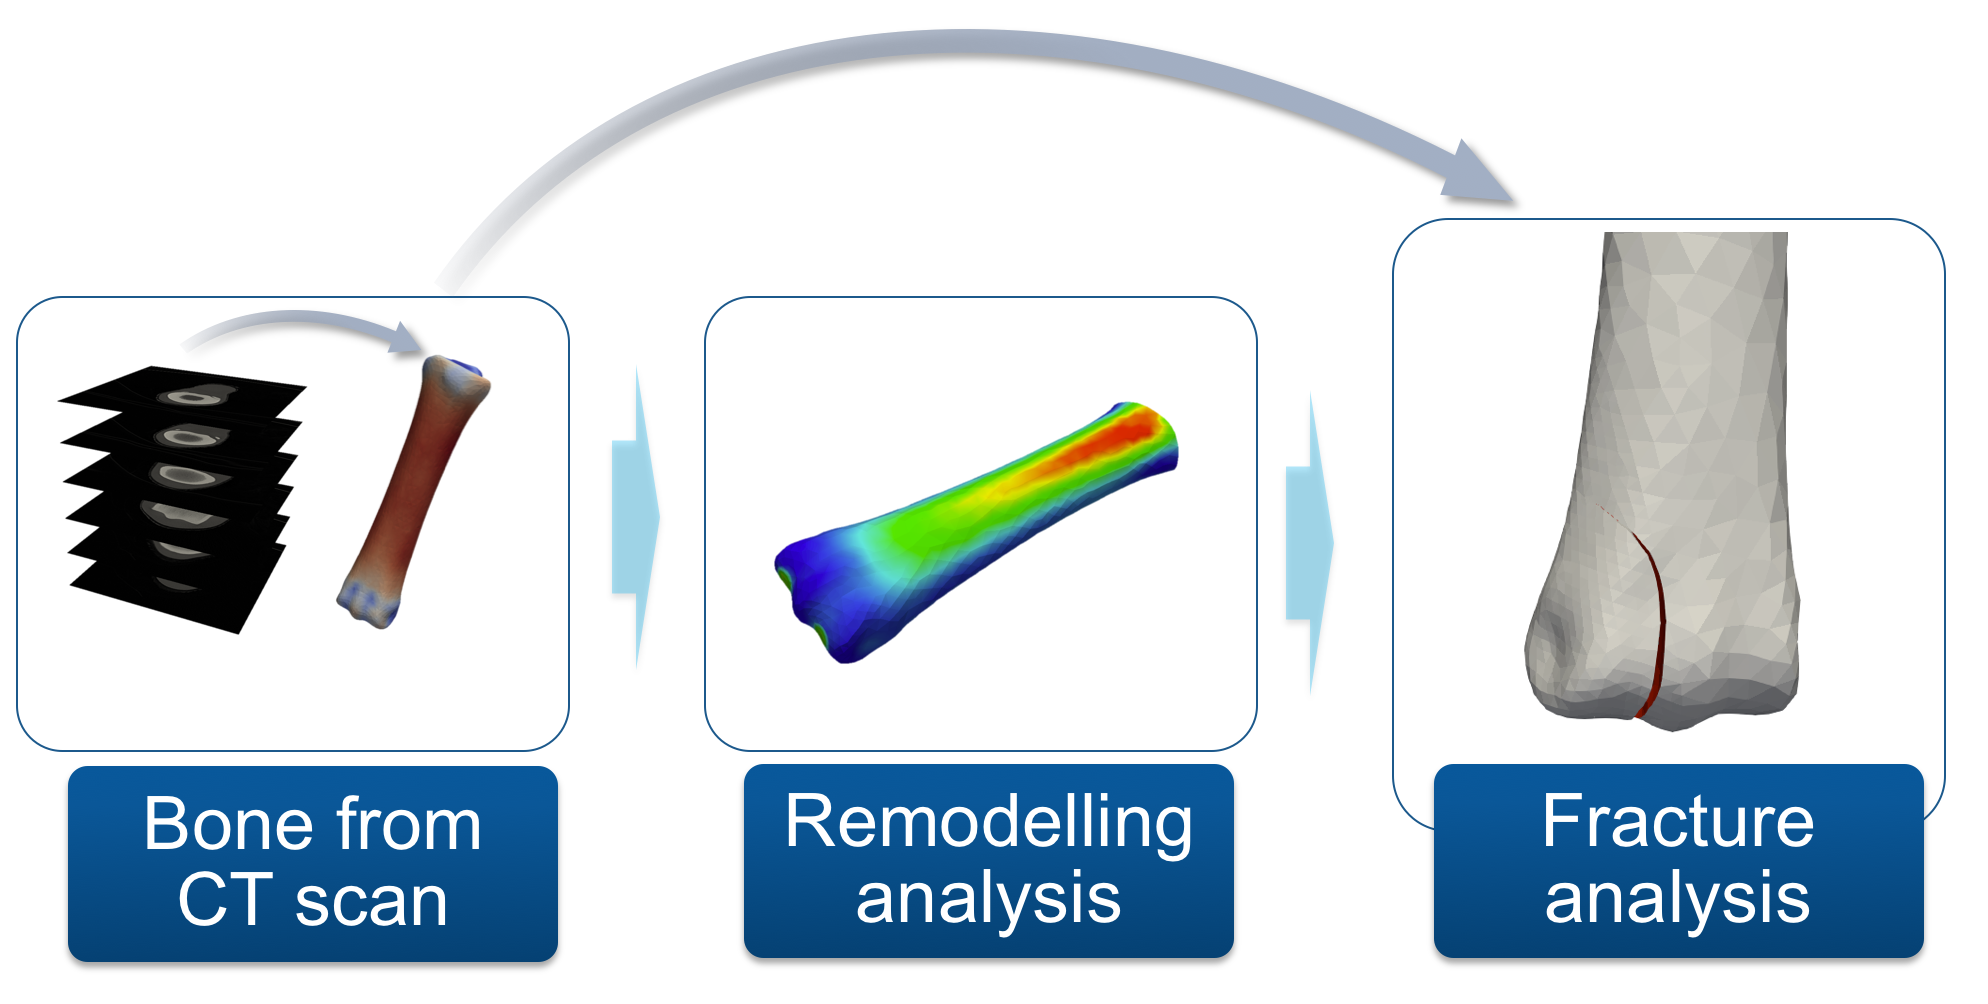
\includegraphics[width=14cm]{Figures/framework.png}};
		\node at(0,0.6){\hspace{1cm} a) Density mapping. \hspace{1.3cm} b) Bone remodelling.  \hspace{1cm} c) Crack propagation analysis.  };
\end{tikzpicture}
\caption{Framework for estimating crack propensity in MoFEM~\citep{mofem2017}. a) Density derived from Quantitative Computed Tomography (qCT) is mapped onto finite element mesh, which is subsequently used for bone remodelling analysis~b). 
Next, utilizing the fracture mechanics module the released energy of an initial crack is computed at different time steps~c).}
\label{fig:framework}
\end{figure}

\section{Bone remodelling} 
\label{sec:bone_remodel}
The ability to repair bone micro-damage caused by cyclic loading is essential for maintaining mechanical integrity and, consequently, there is a strong correlation between stress fractures and the remodelling process~\citep{hughes2017role}. One of the first mathematical theories for bone remodelling~\citep{cowin1976bone}, based on open system thermodynamics, has foundations in the theory of poroelasticity. 
Since this concept was introduced in the 1970s, it has become a popular area of interest within the field of modelling biomechanical processes. 
In this approach (unlike classical closed systems), energy, mass, momentum and entropy can cross the boundary of the body and 
be exchanged with its environment. 
Many derivations and enhancements of this approach have been developed over the years. 
For example, researchers were able to capture the functional adaptation of the bones by means of optimisation theory
~\citep{harrigan1996bone, jacobs1995numerical, weinans1992behavior}.
The general concept for density evolution within these approaches is to establish a~mechanical stimuli as a trigger for bone adaptation. 
The stimulus may take the form of stress~\citep{beaupre1990approach, carter1996mechanical, doblare2002anisotropic}, strains~\citep{cowin1976bone} or strain energy density~\citep{weinans1992behavior, kuhl2003theory,kaczmarczyk2011efficient, Connor2017bone}. 
 
In this paper, functional adaptation of the equine 3rd metacarpal bone is modelled based on an approach proposed by Kuhl and Steinmann~\citep{kuhl2003theory}. 
It is based on the theory of poroelasticity and open system thermodynamics with the modification of constitutive equations proposed in Harrigan et al. 
\citep{harrigan1996bone}. 
It has been shown that the model is stable~\citep{kuhl2003computational}, efficient~\citep{kaczmarczyk2011efficient} and capable of 
producing bone mineral density profiles that are quantitatively comparable with DEXA scans following gait analysis~\citep{pang2012computational}. 
Researchers have been able to simulate bone adaptation in human scapula~\citep{liedtke2017computational}, 
tibia~\citep{pang2012computational}, humerus~\citep{taylor2009phenomenon} and femur with various surgical implants~\citep{ambrosi2011perspectives, Connor2017bone} 
and even explore its potential in topology optimization~\citep{waffenschmidt2012application}. 
One of the advantages of these phenomenological models is that they often require a small number of parameters which can be experimentally
determined from, for example, CT imaging~\citep{zadpoor2013open}.

To the best of authors' knowledge, to date there is only one report of equine bones adaptation in a FEM framework~\citep{Wang2016}. 
In that work, a mechanostat micro-scale model of three-dimensional cortical bone remodelling, informed by \emph{in~vivo} equine data, was presented. 
The model used the von Mises stress as a stimulus to control microstructural cortical bone remodelling.
In contrast, the current paper presents a full macro-scale model of equine bone response to mechanical loading, testing an hypothesis that micro-damage and fracture can be modelled at the macroscale by using clinically available CT-scanning data.
The motivation for this work is to generate subject-specific simulations to acquire meaningful insight into bone resistance
 for veterinary practitioners.

\subsection{Kinematics and balance equations}
This section briefly describes the model formulation used to simulate  adaptation of the equine 3D metacarpal bone. For a more detailed outline, including aspects on the implementation of the model in a finite element framework, the reader is referred to the authors' previous work~\cite{lewandowski2017} based on~\citep{kuhl2003computational}.
%
%%The highly nonlinear continuum theory is solved by means of finite element method with hierarchical basis functions implemented in open source library - MoFEM~\citep{mofem2017}.  \\
%
In the present work, three configurations are considered for modelling crack propagation, i.e. reference, material and spatial configuration (see Section~\ref{sec:Kinematics} for more details) with coordinate systems denoted by $\boldsymbol {\rm \upchi}$, $\boldsymbol {\rm X}$ and $\boldsymbol {\rm x}$, respectively. 
Furthermore, gradient operators corresponding to each coordinate system and therefore configuration are denoted as:

\begin{equation}
\nabla_{\boldsymbol {\rm \upchi}} = \dfrac{\partial}{\partial \boldsymbol {\rm \upchi}}, \nabla_{\boldsymbol {\rm X}} = \dfrac{\partial}{\partial \boldsymbol {\rm X}}, \nabla_{\boldsymbol {\rm x}} = \dfrac{\partial}{\partial \boldsymbol {\rm x}}
\label{eq:gradients}
\end{equation}

Following Kuhl and Steinmann~\citep{kuhl2003computational}, for the sake of generality, a nonlinear kinematic formulation was chosen, although bone, in the physiological range, experiences only small strains. 
The motion of material points ${\boldsymbol {\rm X}} \in  \mathcal{B}_t$ of particles of the body in $\Omega_t$ is described by means of mapping ${\boldsymbol {\rm x}} = \varphi({\boldsymbol {\upchi}},t)$. 
The corresponding deformation gradient tensor, $\boldsymbol {\rm F}$, and the right Cauchy-Green deformation tensor $\boldsymbol {\rm C}$  are denoted as follows: 
\begin{equation}
\mathbf{F}=\nabla_{\boldsymbol {\rm X}}\varphi, \quad \mathbf{C}=\mathbf{F}^{\rm T}\mathbf{F}
\end{equation}

Moreover, it is assumed that the rate of change of the time-dependent material density is in equilibrium with the mass flux evaluated as:
\begin{equation}
\frac{\partial\rho}{\partial t}= \nabla_{\boldsymbol {\rm X}} \cdot \mathbf{R} + \mathcal{R}_0
\label{eq:mass_balance}
\end{equation}
where $\rho$ is mass density, $\mathbf{R}$ is the mass flux and $\mathcal{R}_0$ is the locally created mass. However, it is assumed that the mass flux 
$\mathbf{R}$ is zero, such that only the local mass source $\mathcal{R}_0$ contributes to the changes in density. 
The mechanical equilibrium of a solid is represented by the balance of linear momentum which, for the quasi-static case and in the absence of volume forces, takes the following form:
\begin{equation}
\nabla_{\boldsymbol {\rm X}} \cdot \mathbf{{\mathbf{P}}} = 0
\label{eq:momentum_balance}
\end{equation}
where $\mathbf{P}$ denotes the first Piola-Kirchhoff stress tensor. 
The mechanical forces should be interpreted as an average daily loading on the bone~\citep{kuhl2003computational}, with an additional assumption that inertia forces are negligible. 


\subsection{Constitutive equations}
\label{sec:constitutive_eq}
Following Harrigan and Hamilton~\citep{Harrigan1993}, the constitutive relation for the mass source is:
\begin{equation}
\mathcal{R}_{0}=c\left[\Biggl[\frac{\rho}{\rho_{0}^{\ast}}\Biggr]^{-m}\psi_{0}-\psi_{0}^{\ast}\right]
\label{eq:mass_source}
\end{equation}
where $\rho_0^\ast$ and $\psi_{0}^\ast$ represent reference values of the density, $\rho$ and free energy, $\psi_0$, respectively.  
The driving term $\left[ \rho / \rho_0^\ast \right]^{-m}\psi_0$ tends to converge to $\psi_{0}^\ast$ (see Eq.~(\ref{eq:mass_source})) when density saturation is achieved and locally generated bone mass ceases. 
The exponent $m$ is a dimensionless scalar introduced to guarantee uniqueness and stability~\citep{Harrigan1993} . 
Furthermore, the coefficient $c$ controls the rate of the remodelling process with units~$[\rm{s/cm^2}]$. 
As shown in~\citep{Waffenschmidt2012}, it is beneficial to prescribe an upper and lower bound for bone density, thereby avoiding spurious or non-physical values. In this paper, the constant $c$ is replaced by a bell function defined as:
\begin{equation}
\begin{aligned}
c = & \frac{1}{1 + \left[  (\rho - \rho^{\mathrm{mid}}) / (\rho{^\mathrm{max}} - \rho{^\mathrm{mid})} \right]^{2 b}}\\
& \mathrm{with} \quad \rho^{\mathrm{mid}} = \frac{\rho{^\mathrm{max}} + \rho{^\mathrm{min}}}{2}
\end{aligned}
\label{eq:bell_function}
\end{equation}
%is b an intiger?? please define
%restricting the density between $ \rho{^\mathrm{max}}$ and $ \rho{^\mathrm{min}}$.
where $\rho{^\mathrm{max}}$ and $\rho{^\mathrm{min}}$ are the maximum and minimum values of $\rho$, and $\rho^{\rm {mid}}$ is their average.
The bell function (\ref{eq:bell_function}) is illustrated in Figure~\ref{fig:bell_func} for different values of the integer exponent, $b$. 
Its application and influence on the overall results are elaborated in Section~\ref{sec:numerical_examples:bone_adap}.
\begin{figure}[!htb]
	\centering
		% This file was created by matlab2tikz.
%
%The latest updates can be retrieved from
%  http://www.mathworks.com/matlabcentral/fileexchange/22022-matlab2tikz-matlab2tikz
%where you can also make suggestions and rate matlab2tikz.
%
\definecolor{mycolor1}{rgb}{1.00000,0.00000,1.00000}%
%

\begin{tikzpicture}

\begin{axis}[%
width=5cm,
height=4.5cm,
at={(0cm,0cm)},
scale only axis,
unbounded coords=jump,
xmin=0,
xmax=8,
xtick={0,2,4,6},
xticklabels={{0},{$\rho^\mathrm{min}$},{$\rho^\mathrm{mid}$},{$\rho^\mathrm{max}$}},
xlabel style={font=\color{white!15!black}},
xlabel={$\rho [\mathrm g / \mathrm{cm}^3]$},
ymin=-0.1,
ymax=1.4,
ylabel style={font=\color{white!15!black}},
ylabel={$c [\mathrm s / \mathrm{cm}^2]$},
axis background/.style={fill=white},
legend style={legend cell align=left, align=left, fill=none, draw=none},
legend columns=2
]

\addplot [color=black, line width=2.0pt]
  table[row sep=crcr]{%
0	0.5\\
0.01	0.5\\
0.02	0.5\\
0.03	0.5\\
0.04	0.5\\
0.05	0.5\\
0.06	0.5\\
0.07	0.5\\
0.08	0.5\\
0.09	0.5\\
0.1	0.5\\
0.11	0.5\\
0.12	0.5\\
0.13	0.5\\
0.14	0.5\\
0.15	0.5\\
0.16	0.5\\
0.17	0.5\\
0.18	0.5\\
0.19	0.5\\
0.2	0.5\\
0.21	0.5\\
0.22	0.5\\
0.23	0.5\\
0.24	0.5\\
0.25	0.5\\
0.26	0.5\\
0.27	0.5\\
0.28	0.5\\
0.29	0.5\\
0.3	0.5\\
0.31	0.5\\
0.32	0.5\\
0.33	0.5\\
0.34	0.5\\
0.35	0.5\\
0.36	0.5\\
0.37	0.5\\
0.38	0.5\\
0.39	0.5\\
0.4	0.5\\
0.41	0.5\\
0.42	0.5\\
0.43	0.5\\
0.44	0.5\\
0.45	0.5\\
0.46	0.5\\
0.47	0.5\\
0.48	0.5\\
0.49	0.5\\
0.5	0.5\\
0.51	0.5\\
0.52	0.5\\
0.53	0.5\\
0.54	0.5\\
0.55	0.5\\
0.56	0.5\\
0.57	0.5\\
0.58	0.5\\
0.59	0.5\\
0.6	0.5\\
0.61	0.5\\
0.62	0.5\\
0.63	0.5\\
0.64	0.5\\
0.65	0.5\\
0.66	0.5\\
0.67	0.5\\
0.68	0.5\\
0.69	0.5\\
0.7	0.5\\
0.71	0.5\\
0.72	0.5\\
0.73	0.5\\
0.74	0.5\\
0.75	0.5\\
0.76	0.5\\
0.77	0.5\\
0.78	0.5\\
0.79	0.5\\
0.8	0.5\\
0.81	0.5\\
0.82	0.5\\
0.83	0.5\\
0.84	0.5\\
0.85	0.5\\
0.86	0.5\\
0.87	0.5\\
0.88	0.5\\
0.89	0.5\\
0.9	0.5\\
0.91	0.5\\
0.92	0.5\\
0.93	0.5\\
0.94	0.5\\
0.95	0.5\\
0.96	0.5\\
0.97	0.5\\
0.98	0.5\\
0.99	0.5\\
1	0.5\\
1.01	0.5\\
1.02	0.5\\
1.03	0.5\\
1.04	0.5\\
1.05	0.5\\
1.06	0.5\\
1.07	0.5\\
1.08	0.5\\
1.09	0.5\\
1.1	0.5\\
1.11	0.5\\
1.12	0.5\\
1.13	0.5\\
1.14	0.5\\
1.15	0.5\\
1.16	0.5\\
1.17	0.5\\
1.18	0.5\\
1.19	0.5\\
1.2	0.5\\
1.21	0.5\\
1.22	0.5\\
1.23	0.5\\
1.24	0.5\\
1.25	0.5\\
1.26	0.5\\
1.27	0.5\\
1.28	0.5\\
1.29	0.5\\
1.3	0.5\\
1.31	0.5\\
1.32	0.5\\
1.33	0.5\\
1.34	0.5\\
1.35	0.5\\
1.36	0.5\\
1.37	0.5\\
1.38	0.5\\
1.39	0.5\\
1.4	0.5\\
1.41	0.5\\
1.42	0.5\\
1.43	0.5\\
1.44	0.5\\
1.45	0.5\\
1.46	0.5\\
1.47	0.5\\
1.48	0.5\\
1.49	0.5\\
1.5	0.5\\
1.51	0.5\\
1.52	0.5\\
1.53	0.5\\
1.54	0.5\\
1.55	0.5\\
1.56	0.5\\
1.57	0.5\\
1.58	0.5\\
1.59	0.5\\
1.6	0.5\\
1.61	0.5\\
1.62	0.5\\
1.63	0.5\\
1.64	0.5\\
1.65	0.5\\
1.66	0.5\\
1.67	0.5\\
1.68	0.5\\
1.69	0.5\\
1.7	0.5\\
1.71	0.5\\
1.72	0.5\\
1.73	0.5\\
1.74	0.5\\
1.75	0.5\\
1.76	0.5\\
1.77	0.5\\
1.78	0.5\\
1.79	0.5\\
1.8	0.5\\
1.81	0.5\\
1.82	0.5\\
1.83	0.5\\
1.84	0.5\\
1.85	0.5\\
1.86	0.5\\
1.87	0.5\\
1.88	0.5\\
1.89	0.5\\
1.9	0.5\\
1.91	0.5\\
1.92	0.5\\
1.93	0.5\\
1.94	0.5\\
1.95	0.5\\
1.96	0.5\\
1.97	0.5\\
1.98	0.5\\
1.99	0.5\\
2	0.5\\
2.01	0.5\\
2.02	0.5\\
2.03	0.5\\
2.04	0.5\\
2.05	0.5\\
2.06	0.5\\
2.07	0.5\\
2.08	0.5\\
2.09	0.5\\
2.1	0.5\\
2.11	0.5\\
2.12	0.5\\
2.13	0.5\\
2.14	0.5\\
2.15	0.5\\
2.16	0.5\\
2.17	0.5\\
2.18	0.5\\
2.19	0.5\\
2.2	0.5\\
2.21	0.5\\
2.22	0.5\\
2.23	0.5\\
2.24	0.5\\
2.25	0.5\\
2.26	0.5\\
2.27	0.5\\
2.28	0.5\\
2.29	0.5\\
2.3	0.5\\
2.31	0.5\\
2.32	0.5\\
2.33	0.5\\
2.34	0.5\\
2.35	0.5\\
2.36	0.5\\
2.37	0.5\\
2.38	0.5\\
2.39	0.5\\
2.4	0.5\\
2.41	0.5\\
2.42	0.5\\
2.43	0.5\\
2.44	0.5\\
2.45	0.5\\
2.46	0.5\\
2.47	0.5\\
2.48	0.5\\
2.49	0.5\\
2.5	0.5\\
2.51	0.5\\
2.52	0.5\\
2.53	0.5\\
2.54	0.5\\
2.55	0.5\\
2.56	0.5\\
2.57	0.5\\
2.58	0.5\\
2.59	0.5\\
2.6	0.5\\
2.61	0.5\\
2.62	0.5\\
2.63	0.5\\
2.64	0.5\\
2.65	0.5\\
2.66	0.5\\
2.67	0.5\\
2.68	0.5\\
2.69	0.5\\
2.7	0.5\\
2.71	0.5\\
2.72	0.5\\
2.73	0.5\\
2.74	0.5\\
2.75	0.5\\
2.76	0.5\\
2.77	0.5\\
2.78	0.5\\
2.79	0.5\\
2.8	0.5\\
2.81	0.5\\
2.82	0.5\\
2.83	0.5\\
2.84	0.5\\
2.85	0.5\\
2.86	0.5\\
2.87	0.5\\
2.88	0.5\\
2.89	0.5\\
2.9	0.5\\
2.91	0.5\\
2.92	0.5\\
2.93	0.5\\
2.94	0.5\\
2.95	0.5\\
2.96	0.5\\
2.97	0.5\\
2.98	0.5\\
2.99	0.5\\
3	0.5\\
3.01	0.5\\
3.02	0.5\\
3.03	0.5\\
3.04	0.5\\
3.05	0.5\\
3.06	0.5\\
3.07	0.5\\
3.08	0.5\\
3.09	0.5\\
3.1	0.5\\
3.11	0.5\\
3.12	0.5\\
3.13	0.5\\
3.14	0.5\\
3.15	0.5\\
3.16	0.5\\
3.17	0.5\\
3.18	0.5\\
3.19	0.5\\
3.2	0.5\\
3.21	0.5\\
3.22	0.5\\
3.23	0.5\\
3.24	0.5\\
3.25	0.5\\
3.26	0.5\\
3.27	0.5\\
3.28	0.5\\
3.29	0.5\\
3.3	0.5\\
3.31	0.5\\
3.32	0.5\\
3.33	0.5\\
3.34	0.5\\
3.35	0.5\\
3.36	0.5\\
3.37	0.5\\
3.38	0.5\\
3.39	0.5\\
3.4	0.5\\
3.41	0.5\\
3.42	0.5\\
3.43	0.5\\
3.44	0.5\\
3.45	0.5\\
3.46	0.5\\
3.47	0.5\\
3.48	0.5\\
3.49	0.5\\
3.5	0.5\\
3.51	0.5\\
3.52	0.5\\
3.53	0.5\\
3.54	0.5\\
3.55	0.5\\
3.56	0.5\\
3.57	0.5\\
3.58	0.5\\
3.59	0.5\\
3.6	0.5\\
3.61	0.5\\
3.62	0.5\\
3.63	0.5\\
3.64	0.5\\
3.65	0.5\\
3.66	0.5\\
3.67	0.5\\
3.68	0.5\\
3.69	0.5\\
3.7	0.5\\
3.71	0.5\\
3.72	0.5\\
3.73	0.5\\
3.74	0.5\\
3.75	0.5\\
3.76	0.5\\
3.77	0.5\\
3.78	0.5\\
3.79	0.5\\
3.8	0.5\\
3.81	0.5\\
3.82	0.5\\
3.83	0.5\\
3.84	0.5\\
3.85	0.5\\
3.86	0.5\\
3.87	0.5\\
3.88	0.5\\
3.89	0.5\\
3.9	0.5\\
3.91	0.5\\
3.92	0.5\\
3.93	0.5\\
3.94	0.5\\
3.95	0.5\\
3.96	0.5\\
3.97	0.5\\
3.98	0.5\\
3.99	0.5\\
4	0.5\\
4.01	0.5\\
4.02	0.5\\
4.03	0.5\\
4.04	0.5\\
4.05	0.5\\
4.06	0.5\\
4.07	0.5\\
4.08	0.5\\
4.09	0.5\\
4.1	0.5\\
4.11	0.5\\
4.12	0.5\\
4.13	0.5\\
4.14	0.5\\
4.15	0.5\\
4.16	0.5\\
4.17	0.5\\
4.18	0.5\\
4.19	0.5\\
4.2	0.5\\
4.21	0.5\\
4.22	0.5\\
4.23	0.5\\
4.24	0.5\\
4.25	0.5\\
4.26	0.5\\
4.27	0.5\\
4.28	0.5\\
4.29	0.5\\
4.3	0.5\\
4.31	0.5\\
4.32	0.5\\
4.33	0.5\\
4.34	0.5\\
4.35	0.5\\
4.36	0.5\\
4.37	0.5\\
4.38	0.5\\
4.39	0.5\\
4.4	0.5\\
4.41	0.5\\
4.42	0.5\\
4.43	0.5\\
4.44	0.5\\
4.45	0.5\\
4.46	0.5\\
4.47	0.5\\
4.48	0.5\\
4.49	0.5\\
4.5	0.5\\
4.51	0.5\\
4.52	0.5\\
4.53	0.5\\
4.54	0.5\\
4.55	0.5\\
4.56	0.5\\
4.57	0.5\\
4.58	0.5\\
4.59	0.5\\
4.6	0.5\\
4.61	0.5\\
4.62	0.5\\
4.63	0.5\\
4.64	0.5\\
4.65	0.5\\
4.66	0.5\\
4.67	0.5\\
4.68	0.5\\
4.69	0.5\\
4.7	0.5\\
4.71	0.5\\
4.72	0.5\\
4.73	0.5\\
4.74	0.5\\
4.75	0.5\\
4.76	0.5\\
4.77	0.5\\
4.78	0.5\\
4.79	0.5\\
4.8	0.5\\
4.81	0.5\\
4.82	0.5\\
4.83	0.5\\
4.84	0.5\\
4.85	0.5\\
4.86	0.5\\
4.87	0.5\\
4.88	0.5\\
4.89	0.5\\
4.9	0.5\\
4.91	0.5\\
4.92	0.5\\
4.93	0.5\\
4.94	0.5\\
4.95	0.5\\
4.96	0.5\\
4.97	0.5\\
4.98	0.5\\
4.99	0.5\\
5	0.5\\
5.01	0.5\\
5.02	0.5\\
5.03	0.5\\
5.04	0.5\\
5.05	0.5\\
5.06	0.5\\
5.07	0.5\\
5.08	0.5\\
5.09	0.5\\
5.1	0.5\\
5.11	0.5\\
5.12	0.5\\
5.13	0.5\\
5.14	0.5\\
5.15	0.5\\
5.16	0.5\\
5.17	0.5\\
5.18	0.5\\
5.19	0.5\\
5.2	0.5\\
5.21	0.5\\
5.22	0.5\\
5.23	0.5\\
5.24	0.5\\
5.25	0.5\\
5.26	0.5\\
5.27	0.5\\
5.28	0.5\\
5.29	0.5\\
5.3	0.5\\
5.31	0.5\\
5.32	0.5\\
5.33	0.5\\
5.34	0.5\\
5.35	0.5\\
5.36	0.5\\
5.37	0.5\\
5.38	0.5\\
5.39	0.5\\
5.4	0.5\\
5.41	0.5\\
5.42	0.5\\
5.43	0.5\\
5.44	0.5\\
5.45	0.5\\
5.46	0.5\\
5.47	0.5\\
5.48	0.5\\
5.49	0.5\\
5.5	0.5\\
5.51	0.5\\
5.52	0.5\\
5.53	0.5\\
5.54	0.5\\
5.55	0.5\\
5.56	0.5\\
5.57	0.5\\
5.58	0.5\\
5.59	0.5\\
5.6	0.5\\
5.61	0.5\\
5.62	0.5\\
5.63	0.5\\
5.64	0.5\\
5.65	0.5\\
5.66	0.5\\
5.67	0.5\\
5.68	0.5\\
5.69	0.5\\
5.7	0.5\\
5.71	0.5\\
5.72	0.5\\
5.73	0.5\\
5.74	0.5\\
5.75	0.5\\
5.76	0.5\\
5.77	0.5\\
5.78	0.5\\
5.79	0.5\\
5.8	0.5\\
5.81	0.5\\
5.82	0.5\\
5.83	0.5\\
5.84	0.5\\
5.85	0.5\\
5.86	0.5\\
5.87	0.5\\
5.88	0.5\\
5.89	0.5\\
5.9	0.5\\
5.91	0.5\\
5.92	0.5\\
5.93	0.5\\
5.94	0.5\\
5.95	0.5\\
5.96	0.5\\
5.97	0.5\\
5.98	0.5\\
5.99	0.5\\
6	0.5\\
6.01	0.5\\
6.02	0.5\\
6.03	0.5\\
6.04	0.5\\
6.05	0.5\\
6.06	0.5\\
6.07	0.5\\
6.08	0.5\\
6.09	0.5\\
6.1	0.5\\
6.11	0.5\\
6.12	0.5\\
6.13	0.5\\
6.14	0.5\\
6.15	0.5\\
6.16	0.5\\
6.17	0.5\\
6.18	0.5\\
6.19	0.5\\
6.2	0.5\\
6.21	0.5\\
6.22	0.5\\
6.23	0.5\\
6.24	0.5\\
6.25	0.5\\
6.26	0.5\\
6.27	0.5\\
6.28	0.5\\
6.29	0.5\\
6.3	0.5\\
6.31	0.5\\
6.32	0.5\\
6.33	0.5\\
6.34	0.5\\
6.35	0.5\\
6.36	0.5\\
6.37	0.5\\
6.38	0.5\\
6.39	0.5\\
6.4	0.5\\
6.41	0.5\\
6.42	0.5\\
6.43	0.5\\
6.44	0.5\\
6.45	0.5\\
6.46	0.5\\
6.47	0.5\\
6.48	0.5\\
6.49	0.5\\
6.5	0.5\\
6.51	0.5\\
6.52	0.5\\
6.53	0.5\\
6.54	0.5\\
6.55	0.5\\
6.56	0.5\\
6.57	0.5\\
6.58	0.5\\
6.59	0.5\\
6.6	0.5\\
6.61	0.5\\
6.62	0.5\\
6.63	0.5\\
6.64	0.5\\
6.65	0.5\\
6.66	0.5\\
6.67	0.5\\
6.68	0.5\\
6.69	0.5\\
6.7	0.5\\
6.71	0.5\\
6.72	0.5\\
6.73	0.5\\
6.74	0.5\\
6.75	0.5\\
6.76	0.5\\
6.77	0.5\\
6.78	0.5\\
6.79	0.5\\
6.8	0.5\\
6.81	0.5\\
6.82	0.5\\
6.83	0.5\\
6.84	0.5\\
6.85	0.5\\
6.86	0.5\\
6.87	0.5\\
6.88	0.5\\
6.89	0.5\\
6.9	0.5\\
6.91	0.5\\
6.92	0.5\\
6.93	0.5\\
6.94	0.5\\
6.95	0.5\\
6.96	0.5\\
6.97	0.5\\
6.98	0.5\\
6.99	0.5\\
7	0.5\\
7.01	0.5\\
7.02	0.5\\
7.03	0.5\\
7.04	0.5\\
7.05	0.5\\
7.06	0.5\\
7.07	0.5\\
7.08	0.5\\
7.09	0.5\\
7.1	0.5\\
7.11	0.5\\
7.12	0.5\\
7.13	0.5\\
7.14	0.5\\
7.15	0.5\\
7.16	0.5\\
7.17	0.5\\
7.18	0.5\\
7.19	0.5\\
7.2	0.5\\
7.21	0.5\\
7.22	0.5\\
7.23	0.5\\
7.24	0.5\\
7.25	0.5\\
7.26	0.5\\
7.27	0.5\\
7.28	0.5\\
7.29	0.5\\
7.3	0.5\\
7.31	0.5\\
7.32	0.5\\
7.33	0.5\\
7.34	0.5\\
7.35	0.5\\
7.36	0.5\\
7.37	0.5\\
7.38	0.5\\
7.39	0.5\\
7.4	0.5\\
7.41	0.5\\
7.42	0.5\\
7.43	0.5\\
7.44	0.5\\
7.45	0.5\\
7.46	0.5\\
7.47	0.5\\
7.48	0.5\\
7.49	0.5\\
7.5	0.5\\
7.51	0.5\\
7.52	0.5\\
7.53	0.5\\
7.54	0.5\\
7.55	0.5\\
7.56	0.5\\
7.57	0.5\\
7.58	0.5\\
7.59	0.5\\
7.6	0.5\\
7.61	0.5\\
7.62	0.5\\
7.63	0.5\\
7.64	0.5\\
7.65	0.5\\
7.66	0.5\\
7.67	0.5\\
7.68	0.5\\
7.69	0.5\\
7.7	0.5\\
7.71	0.5\\
7.72	0.5\\
7.73	0.5\\
7.74	0.5\\
7.75	0.5\\
7.76	0.5\\
7.77	0.5\\
7.78	0.5\\
7.79	0.5\\
7.8	0.5\\
7.81	0.5\\
7.82	0.5\\
7.83	0.5\\
7.84	0.5\\
7.85	0.5\\
7.86	0.5\\
7.87	0.5\\
7.88	0.5\\
7.89	0.5\\
7.9	0.5\\
7.91	0.5\\
7.92	0.5\\
7.93	0.5\\
7.94	0.5\\
7.95	0.5\\
7.96	0.5\\
7.97	0.5\\
7.98	0.5\\
7.99	0.5\\
8	0.5\\
};
\addplot [color=black, line width=2.0pt]
  table[row sep=crcr]{%
nan	nan\\
};
\addlegendentry{$b=0$}

\addplot [color=green, dashed, line width=2.0pt]
  table[row sep=crcr]{%
0	0.2\\
0.01	0.200802204808209\\
0.02	0.201608838531481\\
0.03	0.202419930266334\\
0.04	0.203235509308186\\
0.05	0.204055605152404\\
0.06	0.204880247495339\\
0.07	0.205709466235362\\
0.08	0.206543291473893\\
0.09	0.207381753516417\\
0.1	0.208224882873503\\
0.11	0.209072710261811\\
0.12	0.209925266605089\\
0.13	0.210782583035164\\
0.14	0.211644690892929\\
0.15	0.212511621729313\\
0.16	0.213383407306248\\
0.17	0.21426007959762\\
0.18	0.215141670790215\\
0.19	0.216028213284655\\
0.2	0.216919739696312\\
0.21	0.217816282856225\\
0.22	0.21871787581199\\
0.23	0.219624551828649\\
0.24	0.220536344389555\\
0.25	0.221453287197232\\
0.26	0.222375414174209\\
0.27	0.22330275946385\\
0.28	0.22423535743116\\
0.29	0.225173242663574\\
0.3	0.226116449971735\\
0.31	0.227065014390245\\
0.32	0.228018971178402\\
0.33	0.228978355820916\\
0.34	0.229943204028605\\
0.35	0.230913551739068\\
0.36	0.231889435117336\\
0.37	0.232870890556503\\
0.38	0.233857954678328\\
0.39	0.234850664333817\\
0.4	0.235849056603774\\
0.41	0.236853168799332\\
0.42	0.237863038462453\\
0.43	0.238878703366398\\
0.44	0.239900201516169\\
0.45	0.240927571148923\\
0.46	0.241960850734351\\
0.47	0.243000078975026\\
0.48	0.244045294806716\\
0.49	0.245096537398668\\
0.5	0.246153846153846\\
0.51	0.247217260709143\\
0.52	0.248286820935545\\
0.53	0.249362566938264\\
0.54	0.250444539056826\\
0.55	0.251532777865116\\
0.56	0.252627324171382\\
0.57	0.253728219018199\\
0.58	0.254835503682373\\
0.59	0.255949219674816\\
0.6	0.25706940874036\\
0.61	0.258196112857521\\
0.62	0.25932937423822\\
0.63	0.260469235327442\\
0.64	0.261615738802846\\
0.65	0.262768927574314\\
0.66	0.263928844783446\\
0.67	0.265095533802994\\
0.68	0.266269038236234\\
0.69	0.267449401916275\\
0.7	0.268636668905306\\
0.71	0.26983088349377\\
0.72	0.27103209019948\\
0.73	0.272240333766649\\
0.74	0.273455659164866\\
0.75	0.274678111587983\\
0.76	0.27590773645293\\
0.77	0.277144579398458\\
0.78	0.278388686283789\\
0.79	0.279640103187198\\
0.8	0.280898876404494\\
0.81	0.282165052447429\\
0.82	0.283438678042006\\
0.83	0.2847198001267\\
0.84	0.286008465850589\\
0.85	0.287304722571377\\
0.86	0.288608617853329\\
0.87	0.289920199465097\\
0.88	0.291239515377446\\
0.89	0.292566613760871\\
0.9	0.293901542983101\\
0.91	0.295244351606498\\
0.92	0.296595088385336\\
0.93	0.297953802262959\\
0.94	0.299320542368823\\
0.95	0.300695358015411\\
0.96	0.302078298695022\\
0.97	0.303469414076429\\
0.98	0.304868754001402\\
0.99	0.306276368481099\\
1	0.307692307692308\\
1.01	0.309116621973555\\
1.02	0.310549361821061\\
1.03	0.311990577884548\\
1.04	0.313440320962889\\
1.05	0.314898641999606\\
1.06	0.316365592078206\\
1.07	0.317841222417341\\
1.08	0.319325584365819\\
1.09	0.320818729397422\\
1.1	0.32232070910556\\
1.11	0.32383157519774\\
1.12	0.325351379489849\\
1.13	0.326880173900252\\
1.14	0.328418010443693\\
1.15	0.329964941224995\\
1.16	0.331521018432569\\
1.17	0.333086294331704\\
1.18	0.334660821257655\\
1.19	0.33624465160851\\
1.2	0.337837837837838\\
1.21	0.339440432447111\\
1.22	0.3410524879779\\
1.23	0.342674057003829\\
1.24	0.344305192122297\\
1.25	0.345945945945946\\
1.26	0.347596371093886\\
1.27	0.349256520182661\\
1.28	0.350926445816957\\
1.29	0.352606200580037\\
1.3	0.354295837023915\\
1.31	0.355995407659241\\
1.32	0.357704964944913\\
1.33	0.359424561277395\\
1.34	0.361154248979739\\
1.35	0.362894080290315\\
1.36	0.364644107351225\\
1.37	0.366404382196411\\
1.38	0.368174956739443\\
1.39	0.369955882760981\\
1.4	0.371747211895911\\
1.41	0.373548995620138\\
1.42	0.375361285237041\\
1.43	0.377184131863572\\
1.44	0.37901758641601\\
1.45	0.380861699595334\\
1.46	0.382716521872249\\
1.47	0.384582103471815\\
1.48	0.386458494357706\\
1.49	0.388345744216076\\
1.5	0.390243902439024\\
1.51	0.392153018107666\\
1.52	0.394073139974779\\
1.53	0.396004316447049\\
1.54	0.397946595566875\\
1.55	0.399900024993751\\
1.56	0.401864651985211\\
1.57	0.403840523377318\\
1.58	0.405827685564709\\
1.59	0.407826184480175\\
1.6	0.409836065573771\\
1.61	0.411857373791456\\
1.62	0.413890153553247\\
1.63	0.41593444873088\\
1.64	0.417990302624979\\
1.65	0.420057757941717\\
1.66	0.422136856768965\\
1.67	0.42422764055192\\
1.68	0.426330150068213\\
1.69	0.42844442540247\\
1.7	0.430570505920345\\
1.71	0.432708430241992\\
1.72	0.434858236214994\\
1.73	0.437019960886714\\
1.74	0.439193640476086\\
1.75	0.441379310344828\\
1.76	0.443577004968062\\
1.77	0.445786757904357\\
1.78	0.448008601765154\\
1.79	0.450242568183609\\
1.8	0.452488687782805\\
1.81	0.454746990143359\\
1.82	0.457017503770395\\
1.83	0.459300256059893\\
1.84	0.461595273264402\\
1.85	0.463902580458104\\
1.86	0.466222201501236\\
1.87	0.468554159003854\\
1.88	0.470898474288943\\
1.89	0.473255167354859\\
1.9	0.475624256837099\\
1.91	0.478005759969408\\
1.92	0.480399692544197\\
1.93	0.482806068872286\\
1.94	0.485224901741957\\
1.95	0.487656202377324\\
1.96	0.490099980396001\\
1.97	0.492556243766085\\
1.98	0.495024998762437\\
1.99	0.497506249922265\\
2	0.5\\
2.01	0.502506249921484\\
2.02	0.505024998737438\\
2.03	0.507556243576241\\
2.04	0.510099979596001\\
2.05	0.512656199935918\\
2.06	0.515224895666959\\
2.07	0.517806055741822\\
2.08	0.520399666944213\\
2.09	0.523005713837424\\
2.1	0.525624178712221\\
2.11	0.528255041534053\\
2.12	0.530898279889573\\
2.13	0.533553868932492\\
2.14	0.536221781328758\\
2.15	0.538901987201078\\
2.16	0.54159445407279\\
2.17	0.544299146811087\\
2.18	0.547016027569608\\
2.19	0.549745055730405\\
2.2	0.552486187845304\\
2.21	0.555239377576658\\
2.22	0.55800457563752\\
2.23	0.560781729731245\\
2.24	0.563570784490532\\
2.25	0.566371681415929\\
2.26	0.56918435881382\\
2.27	0.572008751733902\\
2.28	0.574844791906185\\
2.29	0.577692407677532\\
2.3	0.58055152394775\\
2.31	0.583422062105279\\
2.32	0.586303939962477\\
2.33	0.589197071690554\\
2.34	0.592101367754159\\
2.35	0.595016734845668\\
2.36	0.597943075819182\\
2.37	0.6008802896243\\
2.38	0.603828271239659\\
2.39	0.606786911606317\\
2.4	0.609756097560976\\
2.41	0.612735711769121\\
2.42	0.615725632658088\\
2.43	0.618725734350106\\
2.44	0.621735886595374\\
2.45	0.624755954705193\\
2.46	0.627785799485216\\
2.47	0.630825277168856\\
2.48	0.633874239350913\\
2.49	0.63693253292145\\
2.5	0.64\\
2.51	0.643076477870131\\
2.52	0.646161798914448\\
2.53	0.649255790550082\\
2.54	0.65235827516472\\
2.55	0.655469070053257\\
2.56	0.658587987355111\\
2.57	0.661714833992291\\
2.58	0.664849411608271\\
2.59	0.66799151650774\\
2.6	0.671140939597315\\
2.61	0.67429746632727\\
2.62	0.677460876634374\\
2.63	0.680630944885909\\
2.64	0.683807439824945\\
2.65	0.68699012451696\\
2.66	0.690178756297881\\
2.67	0.693373086723639\\
2.68	0.696572861521315\\
2.69	0.699777820541978\\
2.7	0.70298769771529\\
2.71	0.706202221005985\\
2.72	0.709421112372304\\
2.73	0.712644087726487\\
2.74	0.715870856897416\\
2.75	0.719101123595506\\
2.76	0.722334585379948\\
2.77	0.725570933628399\\
2.78	0.72880985350922\\
2.79	0.73205102395637\\
2.8	0.735294117647059\\
2.81	0.738538800982257\\
2.82	0.741784734070173\\
2.83	0.745031570712809\\
2.84	0.74827895839569\\
2.85	0.751526538280883\\
2.86	0.754773945203412\\
2.87	0.758020807671171\\
2.88	0.761266747868453\\
2.89	0.764511381663195\\
2.9	0.767754318618042\\
2.91	0.770995162005358\\
2.92	0.774233508826262\\
2.93	0.777468949833816\\
2.94	0.780701069560465\\
2.95	0.783929446349829\\
2.96	0.787153652392947\\
2.97	0.790373253769093\\
2.98	0.793587810491231\\
2.99	0.796796876556244\\
3	0.8\\
3.01	0.80319672295737\\
3.02	0.80638658172728\\
3.03	0.809569106842883\\
3.04	0.812743823146944\\
3.05	0.815910249872514\\
3.06	0.819067900728971\\
3.07	0.822216283993505\\
3.08	0.825354902608121\\
3.09	0.828483254282223\\
3.1	0.831600831600832\\
3.11	0.83470712213852\\
3.12	0.837801608579088\\
3.13	0.840883768841052\\
3.14	0.843953076208963\\
3.15	0.847008999470619\\
3.16	0.850051003060184\\
3.17	0.853078547207234\\
3.18	0.856091088091773\\
3.19	0.859088078005197\\
3.2	0.862068965517241\\
3.21	0.865033195648883\\
3.22	0.867980210051211\\
3.23	0.870909447190228\\
3.24	0.873820342537574\\
3.25	0.876712328767123\\
3.26	0.879584835957428\\
3.27	0.882437291799952\\
3.28	0.885269121813031\\
3.29	0.888079749561511\\
3.3	0.89086859688196\\
3.31	0.893635084113402\\
3.32	0.896378630333453\\
3.33	0.899098653599766\\
3.34	0.901794571196681\\
3.35	0.904465799886942\\
3.36	0.90711175616836\\
3.37	0.909731856535286\\
3.38	0.912325517744731\\
3.39	0.914892157086983\\
3.4	0.91743119266055\\
3.41	0.91994204365125\\
3.42	0.922424130615257\\
3.43	0.924876875765914\\
3.44	0.927299703264095\\
3.45	0.929692039511912\\
3.46	0.932053313449529\\
3.47	0.934382956854867\\
3.48	0.936680404645935\\
3.49	0.938945095185559\\
3.5	0.941176470588235\\
3.51	0.943373977028844\\
3.52	0.94553706505295\\
3.53	0.947665189888413\\
3.54	0.949757811758002\\
3.55	0.951814396192742\\
3.56	0.95383441434567\\
3.57	0.955817343305694\\
3.58	0.957762666411263\\
3.59	0.959669873563494\\
3.6	0.961538461538461\\
3.61	0.963367934298307\\
3.62	0.96515780330084\\
3.63	0.966907587807295\\
3.64	0.968616815187912\\
3.65	0.970285021224985\\
3.66	0.971911750413063\\
3.67	0.973496556255932\\
3.68	0.975039001560062\\
3.69	0.976538658724152\\
3.7	0.97799511002445\\
3.71	0.979407947895497\\
3.72	0.980776775205963\\
3.73	0.98210120552923\\
3.74	0.983380863408398\\
3.75	0.984615384615385\\
3.76	0.985804416403785\\
3.77	0.986947617755188\\
3.78	0.988044659618615\\
3.79	0.989095225142801\\
3.8	0.99009900990099\\
3.81	0.991055722107975\\
3.82	0.991965082829084\\
3.83	0.992826826180843\\
3.84	0.993640699523052\\
3.85	0.994406463642014\\
3.86	0.995123892924669\\
3.87	0.995792775523414\\
3.88	0.996412913511359\\
3.89	0.996984123027841\\
3.9	0.997506234413965\\
3.91	0.997979092338016\\
3.92	0.998402555910543\\
3.93	0.998776498788983\\
3.94	0.999100809271656\\
3.95	0.999375390381012\\
3.96	0.999600159936026\\
3.97	0.999775050613612\\
3.98	0.999900009999\\
3.99	0.999975000624984\\
4	1\\
4.01	0.999975000624984\\
4.02	0.999900009999\\
4.03	0.999775050613612\\
4.04	0.999600159936026\\
4.05	0.999375390381012\\
4.06	0.999100809271655\\
4.07	0.998776498788983\\
4.08	0.998402555910543\\
4.09	0.997979092338016\\
4.1	0.997506234413965\\
4.11	0.996984123027841\\
4.12	0.996412913511359\\
4.13	0.995792775523414\\
4.14	0.995123892924669\\
4.15	0.994406463642014\\
4.16	0.993640699523052\\
4.17	0.992826826180843\\
4.18	0.991965082829084\\
4.19	0.991055722107975\\
4.2	0.99009900990099\\
4.21	0.989095225142801\\
4.22	0.988044659618615\\
4.23	0.986947617755188\\
4.24	0.985804416403785\\
4.25	0.984615384615385\\
4.26	0.983380863408398\\
4.27	0.98210120552923\\
4.28	0.980776775205963\\
4.29	0.979407947895497\\
4.3	0.97799511002445\\
4.31	0.976538658724152\\
4.32	0.975039001560062\\
4.33	0.973496556255932\\
4.34	0.971911750413063\\
4.35	0.970285021224985\\
4.36	0.968616815187912\\
4.37	0.966907587807295\\
4.38	0.96515780330084\\
4.39	0.963367934298307\\
4.4	0.961538461538461\\
4.41	0.959669873563494\\
4.42	0.957762666411263\\
4.43	0.955817343305694\\
4.44	0.95383441434567\\
4.45	0.951814396192742\\
4.46	0.949757811758002\\
4.47	0.947665189888413\\
4.48	0.94553706505295\\
4.49	0.943373977028844\\
4.5	0.941176470588235\\
4.51	0.938945095185559\\
4.52	0.936680404645935\\
4.53	0.934382956854867\\
4.54	0.932053313449529\\
4.55	0.929692039511912\\
4.56	0.927299703264095\\
4.57	0.924876875765914\\
4.58	0.922424130615257\\
4.59	0.91994204365125\\
4.6	0.917431192660551\\
4.61	0.914892157086983\\
4.62	0.912325517744731\\
4.63	0.909731856535286\\
4.64	0.90711175616836\\
4.65	0.904465799886942\\
4.66	0.901794571196681\\
4.67	0.899098653599766\\
4.68	0.896378630333453\\
4.69	0.893635084113403\\
4.7	0.89086859688196\\
4.71	0.888079749561511\\
4.72	0.885269121813031\\
4.73	0.882437291799951\\
4.74	0.879584835957428\\
4.75	0.876712328767123\\
4.76	0.873820342537574\\
4.77	0.870909447190229\\
4.78	0.867980210051211\\
4.79	0.865033195648883\\
4.8	0.862068965517241\\
4.81	0.859088078005197\\
4.82	0.856091088091773\\
4.83	0.853078547207234\\
4.84	0.850051003060184\\
4.85	0.847008999470619\\
4.86	0.843953076208963\\
4.87	0.840883768841052\\
4.88	0.837801608579088\\
4.89	0.834707122138519\\
4.9	0.831600831600832\\
4.91	0.828483254282223\\
4.92	0.825354902608121\\
4.93	0.822216283993505\\
4.94	0.819067900728971\\
4.95	0.815910249872514\\
4.96	0.812743823146944\\
4.97	0.809569106842883\\
4.98	0.80638658172728\\
4.99	0.80319672295737\\
5	0.8\\
5.01	0.796796876556244\\
5.02	0.793587810491231\\
5.03	0.790373253769093\\
5.04	0.787153652392947\\
5.05	0.783929446349829\\
5.06	0.780701069560465\\
5.07	0.777468949833816\\
5.08	0.774233508826262\\
5.09	0.770995162005358\\
5.1	0.767754318618042\\
5.11	0.764511381663195\\
5.12	0.761266747868453\\
5.13	0.758020807671171\\
5.14	0.754773945203411\\
5.15	0.751526538280883\\
5.16	0.74827895839569\\
5.17	0.745031570712809\\
5.18	0.741784734070173\\
5.19	0.738538800982257\\
5.2	0.735294117647059\\
5.21	0.73205102395637\\
5.22	0.72880985350922\\
5.23	0.725570933628399\\
5.24	0.722334585379948\\
5.25	0.719101123595506\\
5.26	0.715870856897416\\
5.27	0.712644087726487\\
5.28	0.709421112372304\\
5.29	0.706202221005985\\
5.3	0.70298769771529\\
5.31	0.699777820541978\\
5.32	0.696572861521315\\
5.33	0.693373086723639\\
5.34	0.690178756297881\\
5.35	0.68699012451696\\
5.36	0.683807439824945\\
5.37	0.680630944885909\\
5.38	0.677460876634374\\
5.39	0.67429746632727\\
5.4	0.671140939597315\\
5.41	0.66799151650774\\
5.42	0.664849411608271\\
5.43	0.661714833992291\\
5.44	0.658587987355111\\
5.45	0.655469070053257\\
5.46	0.65235827516472\\
5.47	0.649255790550082\\
5.48	0.646161798914448\\
5.49	0.643076477870131\\
5.5	0.64\\
5.51	0.63693253292145\\
5.52	0.633874239350913\\
5.53	0.630825277168856\\
5.54	0.627785799485216\\
5.55	0.624755954705193\\
5.56	0.621735886595374\\
5.57	0.618725734350106\\
5.58	0.615725632658088\\
5.59	0.612735711769121\\
5.6	0.609756097560976\\
5.61	0.606786911606317\\
5.62	0.603828271239659\\
5.63	0.6008802896243\\
5.64	0.597943075819182\\
5.65	0.595016734845667\\
5.66	0.592101367754159\\
5.67	0.589197071690554\\
5.68	0.586303939962477\\
5.69	0.583422062105279\\
5.7	0.580551523947751\\
5.71	0.577692407677532\\
5.72	0.574844791906185\\
5.73	0.572008751733901\\
5.74	0.56918435881382\\
5.75	0.566371681415929\\
5.76	0.563570784490532\\
5.77	0.560781729731246\\
5.78	0.55800457563752\\
5.79	0.555239377576658\\
5.8	0.552486187845304\\
5.81	0.549745055730405\\
5.82	0.547016027569608\\
5.83	0.544299146811087\\
5.84	0.54159445407279\\
5.85	0.538901987201078\\
5.86	0.536221781328758\\
5.87	0.533553868932492\\
5.88	0.530898279889573\\
5.89	0.528255041534052\\
5.9	0.525624178712221\\
5.91	0.523005713837424\\
5.92	0.520399666944213\\
5.93	0.517806055741822\\
5.94	0.515224895666959\\
5.95	0.512656199935918\\
5.96	0.510099979596001\\
5.97	0.507556243576241\\
5.98	0.505024998737437\\
5.99	0.502506249921483\\
6	0.5\\
6.01	0.497506249922265\\
6.02	0.495024998762438\\
6.03	0.492556243766085\\
6.04	0.490099980396001\\
6.05	0.487656202377324\\
6.06	0.485224901741957\\
6.07	0.482806068872286\\
6.08	0.480399692544197\\
6.09	0.478005759969408\\
6.1	0.475624256837099\\
6.11	0.473255167354859\\
6.12	0.470898474288943\\
6.13	0.468554159003854\\
6.14	0.466222201501236\\
6.15	0.463902580458104\\
6.16	0.461595273264402\\
6.17	0.459300256059893\\
6.18	0.457017503770395\\
6.19	0.454746990143359\\
6.2	0.452488687782805\\
6.21	0.450242568183609\\
6.22	0.448008601765154\\
6.23	0.445786757904356\\
6.24	0.443577004968062\\
6.25	0.441379310344828\\
6.26	0.439193640476086\\
6.27	0.437019960886714\\
6.28	0.434858236214994\\
6.29	0.432708430241992\\
6.3	0.430570505920345\\
6.31	0.42844442540247\\
6.32	0.426330150068213\\
6.33	0.42422764055192\\
6.34	0.422136856768965\\
6.35	0.420057757941717\\
6.36	0.417990302624979\\
6.37	0.41593444873088\\
6.38	0.413890153553247\\
6.39	0.411857373791456\\
6.4	0.40983606557377\\
6.41	0.407826184480175\\
6.42	0.405827685564709\\
6.43	0.403840523377318\\
6.44	0.401864651985211\\
6.45	0.399900024993751\\
6.46	0.397946595566875\\
6.47	0.396004316447049\\
6.48	0.394073139974779\\
6.49	0.392153018107666\\
6.5	0.390243902439024\\
6.51	0.388345744216076\\
6.52	0.386458494357706\\
6.53	0.384582103471815\\
6.54	0.382716521872249\\
6.55	0.380861699595334\\
6.56	0.37901758641601\\
6.57	0.377184131863572\\
6.58	0.375361285237041\\
6.59	0.373548995620138\\
6.6	0.371747211895911\\
6.61	0.369955882760981\\
6.62	0.368174956739443\\
6.63	0.366404382196411\\
6.64	0.364644107351225\\
6.65	0.362894080290315\\
6.66	0.361154248979739\\
6.67	0.359424561277395\\
6.68	0.357704964944913\\
6.69	0.355995407659241\\
6.7	0.354295837023915\\
6.71	0.352606200580037\\
6.72	0.350926445816957\\
6.73	0.349256520182661\\
6.74	0.347596371093886\\
6.75	0.345945945945946\\
6.76	0.344305192122297\\
6.77	0.342674057003829\\
6.78	0.3410524879779\\
6.79	0.339440432447111\\
6.8	0.337837837837838\\
6.81	0.33624465160851\\
6.82	0.334660821257655\\
6.83	0.333086294331704\\
6.84	0.331521018432569\\
6.85	0.329964941224995\\
6.86	0.328418010443693\\
6.87	0.326880173900252\\
6.88	0.325351379489849\\
6.89	0.32383157519774\\
6.9	0.32232070910556\\
6.91	0.320818729397422\\
6.92	0.319325584365819\\
6.93	0.317841222417341\\
6.94	0.316365592078206\\
6.95	0.314898641999606\\
6.96	0.313440320962889\\
6.97	0.311990577884548\\
6.98	0.310549361821061\\
6.99	0.309116621973555\\
7	0.307692307692308\\
7.01	0.306276368481099\\
7.02	0.304868754001402\\
7.03	0.303469414076429\\
7.04	0.302078298695022\\
7.05	0.300695358015411\\
7.06	0.299320542368823\\
7.07	0.297953802262959\\
7.08	0.296595088385336\\
7.09	0.295244351606498\\
7.1	0.293901542983101\\
7.11	0.292566613760871\\
7.12	0.291239515377446\\
7.13	0.289920199465097\\
7.14	0.288608617853329\\
7.15	0.287304722571377\\
7.16	0.286008465850589\\
7.17	0.2847198001267\\
7.18	0.283438678042006\\
7.19	0.282165052447429\\
7.2	0.280898876404494\\
7.21	0.279640103187198\\
7.22	0.278388686283789\\
7.23	0.277144579398458\\
7.24	0.27590773645293\\
7.25	0.274678111587983\\
7.26	0.273455659164866\\
7.27	0.272240333766649\\
7.28	0.27103209019948\\
7.29	0.26983088349377\\
7.3	0.268636668905306\\
7.31	0.267449401916275\\
7.32	0.266269038236234\\
7.33	0.265095533802994\\
7.34	0.263928844783446\\
7.35	0.262768927574314\\
7.36	0.261615738802846\\
7.37	0.260469235327442\\
7.38	0.25932937423822\\
7.39	0.258196112857521\\
7.4	0.25706940874036\\
7.41	0.255949219674816\\
7.42	0.254835503682373\\
7.43	0.253728219018199\\
7.44	0.252627324171382\\
7.45	0.251532777865116\\
7.46	0.250444539056826\\
7.47	0.249362566938264\\
7.48	0.248286820935545\\
7.49	0.247217260709143\\
7.5	0.246153846153846\\
7.51	0.245096537398668\\
7.52	0.244045294806716\\
7.53	0.243000078975026\\
7.54	0.241960850734351\\
7.55	0.240927571148923\\
7.56	0.239900201516169\\
7.57	0.238878703366398\\
7.58	0.237863038462453\\
7.59	0.236853168799332\\
7.6	0.235849056603774\\
7.61	0.234850664333817\\
7.62	0.233857954678328\\
7.63	0.232870890556503\\
7.64	0.231889435117336\\
7.65	0.230913551739068\\
7.66	0.229943204028605\\
7.67	0.228978355820916\\
7.68	0.228018971178402\\
7.69	0.227065014390245\\
7.7	0.226116449971735\\
7.71	0.225173242663574\\
7.72	0.22423535743116\\
7.73	0.22330275946385\\
7.74	0.222375414174209\\
7.75	0.221453287197232\\
7.76	0.220536344389555\\
7.77	0.219624551828649\\
7.78	0.21871787581199\\
7.79	0.217816282856225\\
7.8	0.216919739696312\\
7.81	0.216028213284655\\
7.82	0.215141670790215\\
7.83	0.21426007959762\\
7.84	0.213383407306248\\
7.85	0.212511621729313\\
7.86	0.211644690892929\\
7.87	0.210782583035164\\
7.88	0.209925266605089\\
7.89	0.209072710261811\\
7.9	0.208224882873503\\
7.91	0.207381753516417\\
7.92	0.206543291473893\\
7.93	0.205709466235363\\
7.94	0.204880247495339\\
7.95	0.204055605152404\\
7.96	0.203235509308186\\
7.97	0.202419930266334\\
7.98	0.201608838531481\\
7.99	0.200802204808209\\
8	0.2\\
};
\addplot [color=green, dashed, line width=2.0pt]
  table[row sep=crcr]{%
nan	nan\\
};
\addlegendentry{$b=1$}

\addplot [color=blue, dotted, line width=2.0pt ]
  table[row sep=crcr]{%
0	0.000975609756097561\\
0.01	0.0010003140101966\\
0.02	0.001025707540306\\
0.03	0.00105181134953671\\
0.04	0.00107864713445174\\
0.05	0.00110623730969214\\
0.06	0.00113460503353668\\
0.07	0.00116377423443281\\
0.08	0.00119376963853799\\
0.09	0.00122461679831213\\
0.1	0.00125634212220359\\
0.11	0.00128897290547305\\
0.12	0.00132253736220131\\
0.13	0.00135706465852924\\
0.14	0.00139258494717988\\
0.15	0.00142912940331515\\
0.16	0.00146673026178155\\
0.17	0.00150542085580168\\
0.18	0.00154523565717105\\
0.19	0.00158621031802169\\
0.2	0.0016283817142173\\
0.21	0.00167178799044699\\
0.22	0.00171646860708777\\
0.23	0.00176246438890894\\
0.24	0.00180981757569466\\
0.25	0.00185857187486415\\
0.26	0.00190877251617264\\
0.27	0.00196046630857964\\
0.28	0.00201370169937465\\
0.29	0.00206852883565472\\
0.3	0.00212499962825208\\
0.31	0.0021831678182143\\
0.32	0.00224308904594399\\
0.33	0.00230482092310965\\
0.34	0.00236842310744409\\
0.35	0.00243395738055187\\
0.36	0.00250148772885242\\
0.37	0.00257108042779131\\
0.38	0.00264280412945718\\
0.39	0.00271672995374877\\
0.4	0.0027929315832417\\
0.41	0.00287148536191208\\
0.42	0.00295247039787999\\
0.43	0.00303596867034363\\
0.44	0.00312206514088177\\
0.45	0.00321084786931022\\
0.46	0.00330240813428561\\
0.47	0.00339684055885859\\
0.48	0.00349424324118679\\
0.49	0.00359471789062728\\
0.5	0.00369836996943731\\
0.51	0.00380530884032245\\
0.52	0.00391564792008072\\
0.53	0.00402950483960258\\
0.54	0.0041470016104973\\
0.55	0.00426826479862781\\
0.56	0.00439342570484795\\
0.57	0.00452262055324853\\
0.58	0.0046559906872315\\
0.59	0.00479368277374462\\
0.6	0.0049358490160231\\
0.61	0.0050826473751989\\
0.62	0.00523424180115327\\
0.63	0.00539080247300344\\
0.64	0.00555250604963045\\
0.65	0.0057195359306712\\
0.66	0.00589208252841539\\
0.67	0.00607034355106492\\
0.68	0.00625452429783192\\
0.69	0.00644483796637004\\
0.7	0.00664150597305277\\
0.71	0.00684475828663244\\
0.72	0.00705483377583372\\
0.73	0.00727198057145633\\
0.74	0.00749645644358264\\
0.75	0.00772852919450809\\
0.76	0.00796847706803405\\
0.77	0.00821658917578558\\
0.78	0.00847316594123937\\
0.79	0.00873851956217052\\
0.8	0.00901297449225012\\
0.81	0.00929686794254935\\
0.82	0.00959055040372947\\
0.83	0.00989438618972087\\
0.84	0.010208754003718\\
0.85	0.0105340475273401\\
0.86	0.0108706760338305\\
0.87	0.0112190650261908\\
0.88	0.0115796569011658\\
0.89	0.0119529116400179\\
0.9	0.0123393075270472\\
0.91	0.0127393418968345\\
0.92	0.0131535319111957\\
0.93	0.0135824153668578\\
0.94	0.0140265515348694\\
0.95	0.0144865220327769\\
0.96	0.0149629317305956\\
0.97	0.0154564096916114\\
0.98	0.0159676101490455\\
0.99	0.0164972135196045\\
1	0.0170459274549298\\
1.01	0.0176144879319369\\
1.02	0.0182036603830092\\
1.03	0.0188142408669793\\
1.04	0.0194470572817823\\
1.05	0.0201029706196147\\
1.06	0.0207828762653667\\
1.07	0.0214877053390163\\
1.08	0.0222184260825841\\
1.09	0.0229760452921357\\
1.1	0.0237616097951991\\
1.11	0.024576207973815\\
1.12	0.0254209713332772\\
1.13	0.0262970761164285\\
1.14	0.0272057449631655\\
1.15	0.0281482486145638\\
1.16	0.0291259076607617\\
1.17	0.0301400943314352\\
1.18	0.0311922343273549\\
1.19	0.0322838086911328\\
1.2	0.0334163557148409\\
1.21	0.0345914728817135\\
1.22	0.0358108188386193\\
1.23	0.0370761153954137\\
1.24	0.0383891495466431\\
1.25	0.0397517755103758\\
1.26	0.0411659167781615\\
1.27	0.042633568169284\\
1.28	0.0441567978815508\\
1.29	0.0457377495298643\\
1.3	0.0473786441627283\\
1.31	0.0490817822456652\\
1.32	0.0508495455992405\\
1.33	0.0526843992780134\\
1.34	0.0545888933752474\\
1.35	0.0565656647366209\\
1.36	0.0586174385644745\\
1.37	0.0607470298923081\\
1.38	0.062957344907308\\
1.39	0.065251382096629\\
1.4	0.0676322331909924\\
1.41	0.0701030838768788\\
1.42	0.0726672142462128\\
1.43	0.0753279989499467\\
1.44	0.0780889070193807\\
1.45	0.0809535013164034\\
1.46	0.0839254375711308\\
1.47	0.0870084629626725\\
1.48	0.0902064141959962\\
1.49	0.0935232150251217\\
1.5	0.0969628731701954\\
1.51	0.100529476573405\\
1.52	0.104227188936261\\
1.53	0.108060244478546\\
1.54	0.112032941857258\\
1.55	0.11614963718228\\
1.56	0.120414736064294\\
1.57	0.124832684629804\\
1.58	0.129407959438068\\
1.59	0.134145056235407\\
1.6	0.139048477483868\\
1.61	0.1441227186037\\
1.62	0.149372252872657\\
1.63	0.15480151492997\\
1.64	0.16041488283897\\
1.65	0.166216658670053\\
1.66	0.172211047574984\\
1.67	0.178402135334648\\
1.68	0.184793864375342\\
1.69	0.191390008263684\\
1.7	0.198194144707314\\
1.71	0.2052096271077\\
1.72	0.21243955473278\\
1.73	0.219886741600569\\
1.74	0.227553684190447\\
1.75	0.235442528126236\\
1.76	0.243555034004356\\
1.77	0.251892542570967\\
1.78	0.26045593948369\\
1.79	0.269245619925915\\
1.8	0.2782614533742\\
1.81	0.287502748851341\\
1.82	0.296968221028615\\
1.83	0.306655957569661\\
1.84	0.316563388134677\\
1.85	0.326687255486127\\
1.86	0.337023589155048\\
1.87	0.347567682139365\\
1.88	0.358314071111349\\
1.89	0.369256520609667\\
1.9	0.380388011681481\\
1.91	0.391700735420961\\
1.92	0.403186091821968\\
1.93	0.414834694323968\\
1.94	0.426636380381377\\
1.95	0.438580228327657\\
1.96	0.450654580736784\\
1.97	0.462847074407103\\
1.98	0.475144677006861\\
1.99	0.487533730328335\\
2	0.5\\
2.01	0.512528731405479\\
2.02	0.525104711456275\\
2.03	0.537712335764764\\
2.04	0.550335680667025\\
2.05	0.562958579454336\\
2.06	0.575564702089852\\
2.07	0.588137637615545\\
2.08	0.600660978395852\\
2.09	0.613118405300458\\
2.1	0.625493772900743\\
2.11	0.637771193743411\\
2.12	0.64993512077142\\
2.13	0.661970426986403\\
2.14	0.673862481487915\\
2.15	0.685597221081947\\
2.16	0.697161216723021\\
2.17	0.708541734138649\\
2.18	0.719726788080196\\
2.19	0.730705189747477\\
2.2	0.741466587043427\\
2.21	0.752001497427057\\
2.22	0.762301333245111\\
2.23	0.772358419532763\\
2.24	0.782166004379058\\
2.25	0.791718262051402\\
2.26	0.801010289163528\\
2.27	0.810038094251466\\
2.28	0.818798581191125\\
2.29	0.827289526948241\\
2.3	0.835509554196568\\
2.31	0.843458099372927\\
2.32	0.851135376758706\\
2.33	0.8585423391869\\
2.34	0.865680635972795\\
2.35	0.872552568655802\\
2.36	0.879161045120871\\
2.37	0.885509532641609\\
2.38	0.891602010354833\\
2.39	0.897442921639198\\
2.4	0.903037126829805\\
2.41	0.908389856657629\\
2.42	0.913506666758137\\
2.43	0.918393393548652\\
2.44	0.923056111729688\\
2.45	0.92750109362235\\
2.46	0.93173477051256\\
2.47	0.935763696133891\\
2.48	0.939594512384443\\
2.49	0.943233917339844\\
2.5	0.946688635594177\\
2.51	0.949965390933607\\
2.52	0.953070881323629\\
2.53	0.956011756170179\\
2.54	0.958794595797217\\
2.55	0.961425893068686\\
2.56	0.963912037070701\\
2.57	0.966259298760405\\
2.58	0.968473818480688\\
2.59	0.970561595234933\\
2.6	0.972528477612677\\
2.61	0.974380156255509\\
2.62	0.976122157752327\\
2.63	0.977759839854152\\
2.64	0.979298387900735\\
2.65	0.980742812354156\\
2.66	0.982097947338193\\
2.67	0.983368450086402\\
2.68	0.984558801206426\\
2.69	0.985673305672874\\
2.7	0.986716094466187\\
2.71	0.98769112678005\\
2.72	0.988602192725058\\
2.73	0.989452916461524\\
2.74	0.990246759699343\\
2.75	0.99098702550775\\
2.76	0.99167686238256\\
2.77	0.992319268523059\\
2.78	0.992917096275033\\
2.79	0.993473056700577\\
2.8	0.993989724239196\\
2.81	0.99446954142838\\
2.82	0.994914823655227\\
2.83	0.995327763913882\\
2.84	0.995710437546513\\
2.85	0.996064806948227\\
2.86	0.996392726218876\\
2.87	0.996695945746972\\
2.88	0.996976116713032\\
2.89	0.997234795501577\\
2.9	0.997473448012761\\
2.91	0.997693453866151\\
2.92	0.997896110490606\\
2.93	0.998082637095459\\
2.94	0.998254178519369\\
2.95	0.998411808954183\\
2.96	0.998556535542086\\
2.97	0.998689301845092\\
2.98	0.998810991186635\\
2.99	0.998922429865626\\
3	0.999024390243902\\
3.01	0.999117593708422\\
3.02	0.999202713509983\\
3.03	0.999280377480579\\
3.04	0.999351170631785\\
3.05	0.999415637636811\\
3.06	0.999474285199065\\
3.07	0.999527584310211\\
3.08	0.999575972400849\\
3.09	0.999619855387033\\
3.1	0.999659609615906\\
3.11	0.999695583713803\\
3.12	0.999728100340148\\
3.13	0.999757457850544\\
3.14	0.999783931872392\\
3.15	0.999807776796375\\
3.16	0.999829227187118\\
3.17	0.999848499116277\\
3.18	0.999865791421259\\
3.19	0.999881286892726\\
3.2	0.999895153393964\\
3.21	0.999907544915114\\
3.22	0.99991860256523\\
3.23	0.999928455504991\\
3.24	0.999937221822867\\
3.25	0.999945009357429\\
3.26	0.999951916468413\\
3.27	0.99995803275908\\
3.28	0.9999634397523\\
3.29	0.999968211522737\\
3.3	0.999972415287402\\
3.31	0.999976111956779\\
3.32	0.999979356648616\\
3.33	0.99998219916644\\
3.34	0.999984684444717\\
3.35	0.999986852962549\\
3.36	0.999988741127695\\
3.37	0.999990381632632\\
3.38	0.999991803784309\\
3.39	0.999993033809156\\
3.4	0.999994095134868\\
3.41	0.99999500865037\\
3.42	0.999995792945366\\
3.43	0.999996464530747\\
3.44	0.999997038041106\\
3.45	0.999997526420551\\
3.46	0.999997941092918\\
3.47	0.999998292117464\\
3.48	0.999998588331036\\
3.49	0.999998837477681\\
3.5	0.999999046326593\\
3.51	0.999999220779257\\
3.52	0.999999365966592\\
3.53	0.999999486336863\\
3.54	0.999999585735059\\
3.55	0.999999667474438\\
3.56	0.999999734400843\\
3.57	0.999999788950413\\
3.58	0.999999833201218\\
3.59	0.99999986891936\\
3.6	0.99999989760001\\
3.61	0.999999920503853\\
3.62	0.999999938689341\\
3.63	0.999999953041171\\
3.64	0.999999964295329\\
3.65	0.999999973061062\\
3.66	0.999999979840061\\
3.67	0.999999985043174\\
3.68	0.999999989004884\\
3.69	0.999999991995818\\
3.7	0.999999994233496\\
3.71	0.999999995891531\\
3.72	0.999999997107453\\
3.73	0.999999997989344\\
3.74	0.999999998621415\\
3.75	0.999999999068677\\
3.76	0.999999999380826\\
3.77	0.999999999595444\\
3.78	0.999999999740626\\
3.79	0.999999999837111\\
3.8	0.9999999999\\
3.81	0.999999999940126\\
3.82	0.999999999965132\\
3.83	0.999999999980313\\
3.84	0.999999999989263\\
3.85	0.999999999994369\\
3.86	0.999999999997175\\
3.87	0.999999999998654\\
3.88	0.999999999999395\\
3.89	0.999999999999747\\
3.9	0.999999999999902\\
3.91	0.999999999999966\\
3.92	0.99999999999999\\
3.93	0.999999999999997\\
3.94	0.999999999999999\\
3.95	1\\
3.96	1\\
3.97	1\\
3.98	1\\
3.99	1\\
4	1\\
4.01	1\\
4.02	1\\
4.03	1\\
4.04	1\\
4.05	1\\
4.06	0.999999999999999\\
4.07	0.999999999999997\\
4.08	0.99999999999999\\
4.09	0.999999999999966\\
4.1	0.999999999999902\\
4.11	0.999999999999747\\
4.12	0.999999999999395\\
4.13	0.999999999998654\\
4.14	0.999999999997175\\
4.15	0.999999999994369\\
4.16	0.999999999989263\\
4.17	0.999999999980313\\
4.18	0.999999999965132\\
4.19	0.999999999940126\\
4.2	0.9999999999\\
4.21	0.999999999837111\\
4.22	0.999999999740626\\
4.23	0.999999999595444\\
4.24	0.999999999380826\\
4.25	0.999999999068677\\
4.26	0.999999998621415\\
4.27	0.999999997989344\\
4.28	0.999999997107453\\
4.29	0.999999995891531\\
4.3	0.999999994233496\\
4.31	0.999999991995818\\
4.32	0.999999989004884\\
4.33	0.999999985043174\\
4.34	0.999999979840061\\
4.35	0.999999973061062\\
4.36	0.999999964295329\\
4.37	0.999999953041171\\
4.38	0.999999938689341\\
4.39	0.999999920503853\\
4.4	0.99999989760001\\
4.41	0.99999986891936\\
4.42	0.999999833201218\\
4.43	0.999999788950413\\
4.44	0.999999734400843\\
4.45	0.999999667474438\\
4.46	0.999999585735059\\
4.47	0.999999486336863\\
4.48	0.999999365966592\\
4.49	0.999999220779257\\
4.5	0.999999046326593\\
4.51	0.999998837477681\\
4.52	0.999998588331036\\
4.53	0.999998292117464\\
4.54	0.999997941092918\\
4.55	0.999997526420551\\
4.56	0.999997038041106\\
4.57	0.999996464530747\\
4.58	0.999995792945366\\
4.59	0.99999500865037\\
4.6	0.999994095134868\\
4.61	0.999993033809156\\
4.62	0.999991803784309\\
4.63	0.999990381632632\\
4.64	0.999988741127695\\
4.65	0.999986852962549\\
4.66	0.999984684444717\\
4.67	0.99998219916644\\
4.68	0.999979356648616\\
4.69	0.999976111956779\\
4.7	0.999972415287402\\
4.71	0.999968211522737\\
4.72	0.9999634397523\\
4.73	0.99995803275908\\
4.74	0.999951916468413\\
4.75	0.999945009357429\\
4.76	0.999937221822867\\
4.77	0.999928455504991\\
4.78	0.99991860256523\\
4.79	0.999907544915114\\
4.8	0.999895153393964\\
4.81	0.999881286892726\\
4.82	0.999865791421259\\
4.83	0.999848499116277\\
4.84	0.999829227187118\\
4.85	0.999807776796375\\
4.86	0.999783931872392\\
4.87	0.999757457850544\\
4.88	0.999728100340148\\
4.89	0.999695583713803\\
4.9	0.999659609615906\\
4.91	0.999619855387033\\
4.92	0.999575972400849\\
4.93	0.999527584310211\\
4.94	0.999474285199065\\
4.95	0.999415637636811\\
4.96	0.999351170631785\\
4.97	0.999280377480579\\
4.98	0.999202713509983\\
4.99	0.999117593708422\\
5	0.999024390243902\\
5.01	0.998922429865626\\
5.02	0.998810991186635\\
5.03	0.998689301845092\\
5.04	0.998556535542086\\
5.05	0.998411808954183\\
5.06	0.998254178519369\\
5.07	0.998082637095459\\
5.08	0.997896110490606\\
5.09	0.997693453866151\\
5.1	0.997473448012761\\
5.11	0.997234795501577\\
5.12	0.996976116713032\\
5.13	0.996695945746972\\
5.14	0.996392726218876\\
5.15	0.996064806948227\\
5.16	0.995710437546513\\
5.17	0.995327763913882\\
5.18	0.994914823655227\\
5.19	0.994469541428381\\
5.2	0.993989724239196\\
5.21	0.993473056700577\\
5.22	0.992917096275033\\
5.23	0.992319268523059\\
5.24	0.99167686238256\\
5.25	0.99098702550775\\
5.26	0.990246759699343\\
5.27	0.989452916461524\\
5.28	0.988602192725058\\
5.29	0.98769112678005\\
5.3	0.986716094466187\\
5.31	0.985673305672874\\
5.32	0.984558801206426\\
5.33	0.983368450086402\\
5.34	0.982097947338193\\
5.35	0.980742812354156\\
5.36	0.979298387900735\\
5.37	0.977759839854152\\
5.38	0.976122157752327\\
5.39	0.974380156255509\\
5.4	0.972528477612677\\
5.41	0.970561595234933\\
5.42	0.968473818480688\\
5.43	0.966259298760405\\
5.44	0.963912037070701\\
5.45	0.961425893068686\\
5.46	0.958794595797217\\
5.47	0.956011756170179\\
5.48	0.953070881323629\\
5.49	0.949965390933607\\
5.5	0.946688635594177\\
5.51	0.943233917339844\\
5.52	0.939594512384443\\
5.53	0.935763696133891\\
5.54	0.93173477051256\\
5.55	0.92750109362235\\
5.56	0.923056111729688\\
5.57	0.918393393548652\\
5.58	0.913506666758137\\
5.59	0.908389856657629\\
5.6	0.903037126829805\\
5.61	0.897442921639198\\
5.62	0.891602010354833\\
5.63	0.885509532641609\\
5.64	0.87916104512087\\
5.65	0.872552568655801\\
5.66	0.865680635972795\\
5.67	0.8585423391869\\
5.68	0.851135376758706\\
5.69	0.843458099372927\\
5.7	0.835509554196569\\
5.71	0.827289526948241\\
5.72	0.818798581191125\\
5.73	0.810038094251466\\
5.74	0.801010289163527\\
5.75	0.791718262051402\\
5.76	0.782166004379058\\
5.77	0.772358419532764\\
5.78	0.762301333245112\\
5.79	0.752001497427057\\
5.8	0.741466587043427\\
5.81	0.730705189747477\\
5.82	0.719726788080196\\
5.83	0.708541734138649\\
5.84	0.697161216723021\\
5.85	0.685597221081948\\
5.86	0.673862481487916\\
5.87	0.661970426986403\\
5.88	0.64993512077142\\
5.89	0.637771193743411\\
5.9	0.625493772900743\\
5.91	0.613118405300458\\
5.92	0.600660978395852\\
5.93	0.588137637615546\\
5.94	0.575564702089852\\
5.95	0.562958579454336\\
5.96	0.550335680667025\\
5.97	0.537712335764764\\
5.98	0.525104711456274\\
5.99	0.512528731405478\\
6	0.5\\
6.01	0.487533730328335\\
6.02	0.475144677006861\\
6.03	0.462847074407103\\
6.04	0.450654580736784\\
6.05	0.438580228327657\\
6.06	0.426636380381377\\
6.07	0.414834694323968\\
6.08	0.403186091821968\\
6.09	0.391700735420961\\
6.1	0.380388011681481\\
6.11	0.369256520609668\\
6.12	0.358314071111349\\
6.13	0.347567682139365\\
6.14	0.337023589155048\\
6.15	0.326687255486126\\
6.16	0.316563388134677\\
6.17	0.306655957569661\\
6.18	0.296968221028615\\
6.19	0.287502748851341\\
6.2	0.2782614533742\\
6.21	0.269245619925915\\
6.22	0.26045593948369\\
6.23	0.251892542570967\\
6.24	0.243555034004356\\
6.25	0.235442528126236\\
6.26	0.227553684190447\\
6.27	0.219886741600569\\
6.28	0.21243955473278\\
6.29	0.2052096271077\\
6.3	0.198194144707314\\
6.31	0.191390008263684\\
6.32	0.184793864375342\\
6.33	0.178402135334648\\
6.34	0.172211047574984\\
6.35	0.166216658670053\\
6.36	0.16041488283897\\
6.37	0.15480151492997\\
6.38	0.149372252872657\\
6.39	0.1441227186037\\
6.4	0.139048477483868\\
6.41	0.134145056235407\\
6.42	0.129407959438068\\
6.43	0.124832684629804\\
6.44	0.120414736064295\\
6.45	0.11614963718228\\
6.46	0.112032941857258\\
6.47	0.108060244478546\\
6.48	0.104227188936261\\
6.49	0.100529476573405\\
6.5	0.0969628731701954\\
6.51	0.0935232150251217\\
6.52	0.0902064141959963\\
6.53	0.0870084629626725\\
6.54	0.0839254375711308\\
6.55	0.0809535013164034\\
6.56	0.0780889070193806\\
6.57	0.0753279989499467\\
6.58	0.0726672142462128\\
6.59	0.0701030838768788\\
6.6	0.0676322331909924\\
6.61	0.0652513820966291\\
6.62	0.062957344907308\\
6.63	0.0607470298923081\\
6.64	0.0586174385644745\\
6.65	0.0565656647366208\\
6.66	0.0545888933752474\\
6.67	0.0526843992780134\\
6.68	0.0508495455992405\\
6.69	0.0490817822456652\\
6.7	0.0473786441627283\\
6.71	0.0457377495298643\\
6.72	0.0441567978815508\\
6.73	0.0426335681692839\\
6.74	0.0411659167781615\\
6.75	0.0397517755103758\\
6.76	0.0383891495466431\\
6.77	0.0370761153954137\\
6.78	0.0358108188386193\\
6.79	0.0345914728817135\\
6.8	0.0334163557148409\\
6.81	0.0322838086911328\\
6.82	0.0311922343273549\\
6.83	0.0301400943314352\\
6.84	0.0291259076607617\\
6.85	0.0281482486145638\\
6.86	0.0272057449631655\\
6.87	0.0262970761164285\\
6.88	0.0254209713332772\\
6.89	0.024576207973815\\
6.9	0.0237616097951991\\
6.91	0.0229760452921357\\
6.92	0.0222184260825841\\
6.93	0.0214877053390163\\
6.94	0.0207828762653667\\
6.95	0.0201029706196147\\
6.96	0.0194470572817823\\
6.97	0.0188142408669793\\
6.98	0.0182036603830091\\
6.99	0.0176144879319369\\
7	0.0170459274549298\\
7.01	0.0164972135196045\\
7.02	0.0159676101490455\\
7.03	0.0154564096916114\\
7.04	0.0149629317305956\\
7.05	0.0144865220327769\\
7.06	0.0140265515348694\\
7.07	0.0135824153668578\\
7.08	0.0131535319111957\\
7.09	0.0127393418968345\\
7.1	0.0123393075270473\\
7.11	0.0119529116400179\\
7.12	0.0115796569011658\\
7.13	0.0112190650261908\\
7.14	0.0108706760338305\\
7.15	0.0105340475273401\\
7.16	0.010208754003718\\
7.17	0.00989438618972087\\
7.18	0.00959055040372947\\
7.19	0.00929686794254937\\
7.2	0.00901297449225012\\
7.21	0.00873851956217052\\
7.22	0.00847316594123937\\
7.23	0.00821658917578556\\
7.24	0.00796847706803405\\
7.25	0.00772852919450809\\
7.26	0.00749645644358264\\
7.27	0.00727198057145634\\
7.28	0.00705483377583372\\
7.29	0.00684475828663244\\
7.3	0.00664150597305277\\
7.31	0.00644483796637005\\
7.32	0.00625452429783192\\
7.33	0.00607034355106492\\
7.34	0.00589208252841539\\
7.35	0.00571953593067121\\
7.36	0.00555250604963044\\
7.37	0.00539080247300344\\
7.38	0.00523424180115327\\
7.39	0.00508264737519891\\
7.4	0.0049358490160231\\
7.41	0.00479368277374462\\
7.42	0.0046559906872315\\
7.43	0.00452262055324853\\
7.44	0.00439342570484795\\
7.45	0.00426826479862781\\
7.46	0.0041470016104973\\
7.47	0.00402950483960258\\
7.48	0.00391564792008071\\
7.49	0.00380530884032245\\
7.5	0.00369836996943731\\
7.51	0.00359471789062728\\
7.52	0.0034942432411868\\
7.53	0.00339684055885858\\
7.54	0.00330240813428561\\
7.55	0.00321084786931022\\
7.56	0.00312206514088177\\
7.57	0.00303596867034362\\
7.58	0.00295247039787999\\
7.59	0.00287148536191208\\
7.6	0.00279293158324171\\
7.61	0.00271672995374876\\
7.62	0.00264280412945718\\
7.63	0.00257108042779131\\
7.64	0.00250148772885243\\
7.65	0.00243395738055186\\
7.66	0.00236842310744409\\
7.67	0.00230482092310965\\
7.68	0.00224308904594399\\
7.69	0.0021831678182143\\
7.7	0.00212499962825208\\
7.71	0.00206852883565472\\
7.72	0.00201370169937465\\
7.73	0.00196046630857964\\
7.74	0.00190877251617264\\
7.75	0.00185857187486415\\
7.76	0.00180981757569466\\
7.77	0.00176246438890895\\
7.78	0.00171646860708776\\
7.79	0.00167178799044699\\
7.8	0.0016283817142173\\
7.81	0.00158621031802169\\
7.82	0.00154523565717104\\
7.83	0.00150542085580168\\
7.84	0.00146673026178155\\
7.85	0.00142912940331515\\
7.86	0.00139258494717988\\
7.87	0.00135706465852924\\
7.88	0.00132253736220131\\
7.89	0.00128897290547305\\
7.9	0.00125634212220359\\
7.91	0.00122461679831213\\
7.92	0.00119376963853799\\
7.93	0.00116377423443281\\
7.94	0.00113460503353668\\
7.95	0.00110623730969214\\
7.96	0.00107864713445174\\
7.97	0.00105181134953671\\
7.98	0.001025707540306\\
7.99	0.0010003140101966\\
8	0.000975609756097561\\
};
\addplot [color=blue, dotted, line width=2.0pt]
  table[row sep=crcr]{%
nan	nan\\
};
\addlegendentry{$b=5$}

\addplot [color=mycolor1, dashdotted, line width=2.0pt]
  table[row sep=crcr]{%
0	8.67361737988404e-19\\
0.01	1.00791985079053e-18\\
0.02	1.17169726293167e-18\\
0.03	1.36260297890052e-18\\
0.04	1.58521650070541e-18\\
0.05	1.84490497611919e-18\\
0.06	2.1479611908287e-18\\
0.07	2.50176618044797e-18\\
0.08	2.91498093463549e-18\\
0.09	3.39777249249907e-18\\
0.1	3.9620807110297e-18\\
0.11	4.62193315626916e-18\\
0.12	5.39381695588771e-18\\
0.13	6.2971181043746e-18\\
0.14	7.3546406790151e-18\\
0.15	8.59322076711882e-18\\
0.16	1.00444526954517e-17\\
0.17	1.17455484787654e-17\\
0.18	1.37403553702715e-17\\
0.19	1.60805611281784e-17\\
0.2	1.88271222592931e-17\\
0.21	2.20519572434629e-17\\
0.22	2.58399547977493e-17\\
0.23	3.0291356866555e-17\\
0.24	3.55245875357652e-17\\
0.25	4.16796128406655e-17\\
0.26	4.89219329204214e-17\\
0.27	5.74473277094115e-17\\
0.28	6.74875010016379e-17\\
0.29	7.93167960663542e-17\\
0.3	9.32601899800124e-17\\
0.31	1.09702814615831e-16\\
0.32	1.29101301177903e-16\\
0.33	1.51997303947399e-16\\
0.34	1.7903362953523e-16\\
0.35	2.10973482838133e-16\\
0.36	2.48723443010041e-16\\
0.37	2.93360905639187e-16\\
0.38	3.46166875260082e-16\\
0.39	4.08665170530163e-16\\
0.4	4.82669319162891e-16\\
0.41	5.70338678667366e-16\\
0.42	6.74245631355003e-16\\
0.43	7.97456079166274e-16\\
0.44	9.43625919273699e-16\\
0.45	1.11711673168412e-15\\
0.46	1.32313457530427e-15\\
0.47	1.56789659360112e-15\\
0.48	1.85883110482161e-15\\
0.49	2.20481803093637e-15\\
0.5	2.6164779481137e-15\\
0.51	3.10651977332572e-15\\
0.52	3.69015920210786e-15\\
0.53	4.38562256140424e-15\\
0.54	5.21475383630696e-15\\
0.55	6.20374638936754e-15\\
0.56	7.38402546146725e-15\\
0.57	8.79331310179094e-15\\
0.58	1.04769139387734e-14\\
0.59	1.24892684402134e-14\\
0.6	1.4895830345145e-14\\
0.61	1.77753371820886e-14\\
0.62	2.12225577079132e-14\\
0.63	2.53516183098171e-14\\
0.64	3.03000326478216e-14\\
0.65	3.62335859830809e-14\\
0.66	4.33522588524004e-14\\
0.67	5.18974153817864e-14\\
0.68	6.21605312678849e-14\\
0.69	7.44937973720921e-14\\
0.7	8.93230095263671e-14\\
0.71	1.07163246696498e-13\\
0.72	1.28637951979188e-13\\
0.73	1.5450216882747e-13\\
0.74	1.85670854338494e-13\\
0.75	2.23253399733101e-13\\
0.76	2.68595744379286e-13\\
0.77	3.23331785088952e-13\\
0.78	3.89446170853753e-13\\
0.79	4.69351051912372e-13\\
0.8	5.65979942426347e-13\\
0.81	6.82902584600072e-13\\
0.82	8.24465601738067e-13\\
0.83	9.95964839400805e-13\\
0.84	1.20385666836888e-12\\
0.85	1.45601722384924e-12\\
0.86	1.76206066106542e-12\\
0.87	2.13373011625872e-12\\
0.88	2.5853782966186e-12\\
0.89	3.13455863551374e-12\\
0.9	3.80275293133467e-12\\
0.91	4.61626757759066e-12\\
0.92	5.60733818658637e-12\\
0.93	6.81549198186439e-12\\
0.94	8.28922925245951e-12\\
0.95	1.00881000098342e-11\\
0.96	1.2285270499661e-11\\
0.97	1.49706973158775e-11\\
0.98	1.8255055699608e-11\\
0.99	2.22746046333754e-11\\
1	2.71972163886246e-11\\
1.01	3.32298545516056e-11\\
1.02	4.06278551357857e-11\\
1.03	4.97064538395738e-11\\
1.04	6.08551134325935e-11\\
1.05	7.45553444675702e-11\\
1.06	9.14028873659704e-11\\
1.07	1.12135343705104e-10\\
1.08	1.37666621000336e-10\\
1.09	1.69129903319589e-10\\
1.1	2.07931298563009e-10\\
1.11	2.55816866131528e-10\\
1.12	3.14956426390746e-10\\
1.13	3.88048434433005e-10\\
1.14	4.78451314263705e-10\\
1.15	5.90348058193428e-10\\
1.16	7.28952679522055e-10\\
1.17	9.00769366051713e-10\\
1.18	1.11391804706262e-09\\
1.19	1.37854372250013e-09\\
1.2	1.70733152160962e-09\\
1.21	2.11615532948419e-09\\
1.22	2.62489529010846e-09\\
1.23	3.25846900705347e-09\\
1.24	4.04813338689965e-09\\
1.25	5.03312953602307e-09\\
1.26	6.26276286688166e-09\\
1.27	7.79903580204392e-09\\
1.28	9.7199827360944e-09\\
1.29	1.21238982282626e-08\\
1.3	1.51347023325562e-08\\
1.31	1.89087548579467e-08\\
1.32	2.36435174916857e-08\\
1.33	2.95885746784944e-08\\
1.34	3.70596681295485e-08\\
1.35	4.64565851694518e-08\\
1.36	5.82859799184976e-08\\
1.37	7.31905142610284e-08\\
1.38	9.19861030814384e-08\\
1.39	1.15709561907634e-07\\
1.4	1.45679619454906e-07\\
1.41	1.83575117661248e-07\\
1.42	2.31535336418906e-07\\
1.43	2.92288826084224e-07\\
1.44	3.69319008314849e-07\\
1.45	4.67077246122271e-07\\
1.46	5.91257259206804e-07\\
1.47	7.49148896157551e-07\\
1.48	9.50094666947272e-07\\
1.49	1.20607947627508e-06\\
1.5	1.53249319232691e-06\\
1.51	1.94911771013311e-06\\
1.52	2.48140591197212e-06\\
1.53	3.1621405610912e-06\\
1.54	4.03358823746201e-06\\
1.55	5.15029898252941e-06\\
1.56	6.5827490739745e-06\\
1.57	8.42208589264697e-06\\
1.58	1.07863149359208e-05\\
1.59	1.38283760005477e-05\\
1.6	1.77466968114272e-05\\
1.61	2.27989990959612e-05\\
1.62	2.93203791901104e-05\\
1.63	3.77470125574918e-05\\
1.64	4.86472655687885e-05\\
1.65	6.27625738271104e-05\\
1.66	8.10612113443393e-05\\
1.67	0.000104809091839712\\
1.68	0.000135663096210384\\
1.69	0.000175794220602066\\
1.7	0.000228050236272093\\
1.71	0.00029617074314905\\
1.72	0.000385071745038435\\
1.73	0.000501222519806131\\
1.74	0.000653145051841057\\
1.75	0.000852076216778562\\
1.76	0.00111284599660827\\
1.77	0.00145504216922131\\
1.78	0.00190455424545771\\
1.79	0.002495618123551\\
1.8	0.00327351915978051\\
1.81	0.00429815587047405\\
1.82	0.00564871887295807\\
1.83	0.00742979690655078\\
1.84	0.00977927552520355\\
1.85	0.0128784260522418\\
1.86	0.0169645566949643\\
1.87	0.0223464487434447\\
1.88	0.0294224166129824\\
1.89	0.0387000342021163\\
1.9	0.0508151102073106\\
1.91	0.0665450758195941\\
1.92	0.086808363202871\\
1.93	0.112636828252634\\
1.94	0.145104119448339\\
1.95	0.185192395726046\\
1.96	0.233588602707018\\
1.97	0.290425841260648\\
1.98	0.35502580043843\\
1.99	0.425740228219607\\
2	0.5\\
2.01	0.574626463679067\\
2.02	0.646346964877932\\
2.03	0.712348641102709\\
2.04	0.770681344060585\\
2.05	0.820401268439434\\
2.06	0.861469895622569\\
2.07	0.894507238748232\\
2.08	0.920511685450744\\
2.09	0.940623046601993\\
2.1	0.955959153938325\\
2.11	0.967523441120422\\
2.12	0.976166109392388\\
2.13	0.982579352771733\\
2.14	0.987310899280241\\
2.15	0.99078525126642\\
2.16	0.993326377924272\\
2.17	0.995178671713536\\
2.18	0.9965248650131\\
2.19	0.997500645050208\\
2.2	0.998206213153524\\
2.21	0.998715234713504\\
2.22	0.9990816644698\\
2.23	0.999344893905574\\
2.24	0.999533600874773\\
2.25	0.999668610123883\\
2.26	0.99976500799358\\
2.27	0.999833699245966\\
2.28	0.999882549177252\\
2.29	0.999917218949975\\
2.3	0.999941774898366\\
2.31	0.999959131867965\\
2.32	0.999971375050321\\
2.33	0.999979993098221\\
2.34	0.999986046618044\\
2.35	0.999990289698923\\
2.36	0.999993257387292\\
2.37	0.999995328519981\\
2.38	0.99999677076441\\
2.39	0.99999777283776\\
2.4	0.999998467506808\\
2.41	0.999998947972088\\
2.42	0.999999279514634\\
2.43	0.999999507757406\\
2.44	0.999999664512753\\
2.45	0.999999771912203\\
2.46	0.999999845316695\\
2.47	0.999999895362811\\
2.48	0.999999929398243\\
2.49	0.999999952486494\\
2.5	0.999999968108438\\
2.51	0.999999978651058\\
2.52	0.999999985747102\\
2.53	0.999999990510565\\
2.54	0.999999993699549\\
2.55	0.999999995828614\\
2.56	0.99999999724609\\
2.57	0.999999998187147\\
2.58	0.999999998810126\\
2.59	0.999999999221342\\
2.6	0.999999999491978\\
2.61	0.999999999669563\\
2.62	0.999999999785738\\
2.63	0.999999999861505\\
2.64	0.999999999910765\\
2.65	0.999999999942691\\
2.66	0.999999999963315\\
2.67	0.999999999976596\\
2.68	0.999999999985119\\
2.69	0.999999999990571\\
2.7	0.999999999994046\\
2.71	0.999999999996254\\
2.72	0.999999999997651\\
2.73	0.999999999998533\\
2.74	0.999999999999087\\
2.75	0.999999999999434\\
2.76	0.999999999999651\\
2.77	0.999999999999785\\
2.78	0.999999999999868\\
2.79	0.99999999999992\\
2.8	0.999999999999951\\
2.81	0.99999999999997\\
2.82	0.999999999999982\\
2.83	0.999999999999989\\
2.84	0.999999999999994\\
2.85	0.999999999999996\\
2.86	0.999999999999998\\
2.87	0.999999999999999\\
2.88	0.999999999999999\\
2.89	1\\
2.9	1\\
2.91	1\\
2.92	1\\
2.93	1\\
2.94	1\\
2.95	1\\
2.96	1\\
2.97	1\\
2.98	1\\
2.99	1\\
3	1\\
3.01	1\\
3.02	1\\
3.03	1\\
3.04	1\\
3.05	1\\
3.06	1\\
3.07	1\\
3.08	1\\
3.09	1\\
3.1	1\\
3.11	1\\
3.12	1\\
3.13	1\\
3.14	1\\
3.15	1\\
3.16	1\\
3.17	1\\
3.18	1\\
3.19	1\\
3.2	1\\
3.21	1\\
3.22	1\\
3.23	1\\
3.24	1\\
3.25	1\\
3.26	1\\
3.27	1\\
3.28	1\\
3.29	1\\
3.3	1\\
3.31	1\\
3.32	1\\
3.33	1\\
3.34	1\\
3.35	1\\
3.36	1\\
3.37	1\\
3.38	1\\
3.39	1\\
3.4	1\\
3.41	1\\
3.42	1\\
3.43	1\\
3.44	1\\
3.45	1\\
3.46	1\\
3.47	1\\
3.48	1\\
3.49	1\\
3.5	1\\
3.51	1\\
3.52	1\\
3.53	1\\
3.54	1\\
3.55	1\\
3.56	1\\
3.57	1\\
3.58	1\\
3.59	1\\
3.6	1\\
3.61	1\\
3.62	1\\
3.63	1\\
3.64	1\\
3.65	1\\
3.66	1\\
3.67	1\\
3.68	1\\
3.69	1\\
3.7	1\\
3.71	1\\
3.72	1\\
3.73	1\\
3.74	1\\
3.75	1\\
3.76	1\\
3.77	1\\
3.78	1\\
3.79	1\\
3.8	1\\
3.81	1\\
3.82	1\\
3.83	1\\
3.84	1\\
3.85	1\\
3.86	1\\
3.87	1\\
3.88	1\\
3.89	1\\
3.9	1\\
3.91	1\\
3.92	1\\
3.93	1\\
3.94	1\\
3.95	1\\
3.96	1\\
3.97	1\\
3.98	1\\
3.99	1\\
4	1\\
4.01	1\\
4.02	1\\
4.03	1\\
4.04	1\\
4.05	1\\
4.06	1\\
4.07	1\\
4.08	1\\
4.09	1\\
4.1	1\\
4.11	1\\
4.12	1\\
4.13	1\\
4.14	1\\
4.15	1\\
4.16	1\\
4.17	1\\
4.18	1\\
4.19	1\\
4.2	1\\
4.21	1\\
4.22	1\\
4.23	1\\
4.24	1\\
4.25	1\\
4.26	1\\
4.27	1\\
4.28	1\\
4.29	1\\
4.3	1\\
4.31	1\\
4.32	1\\
4.33	1\\
4.34	1\\
4.35	1\\
4.36	1\\
4.37	1\\
4.38	1\\
4.39	1\\
4.4	1\\
4.41	1\\
4.42	1\\
4.43	1\\
4.44	1\\
4.45	1\\
4.46	1\\
4.47	1\\
4.48	1\\
4.49	1\\
4.5	1\\
4.51	1\\
4.52	1\\
4.53	1\\
4.54	1\\
4.55	1\\
4.56	1\\
4.57	1\\
4.58	1\\
4.59	1\\
4.6	1\\
4.61	1\\
4.62	1\\
4.63	1\\
4.64	1\\
4.65	1\\
4.66	1\\
4.67	1\\
4.68	1\\
4.69	1\\
4.7	1\\
4.71	1\\
4.72	1\\
4.73	1\\
4.74	1\\
4.75	1\\
4.76	1\\
4.77	1\\
4.78	1\\
4.79	1\\
4.8	1\\
4.81	1\\
4.82	1\\
4.83	1\\
4.84	1\\
4.85	1\\
4.86	1\\
4.87	1\\
4.88	1\\
4.89	1\\
4.9	1\\
4.91	1\\
4.92	1\\
4.93	1\\
4.94	1\\
4.95	1\\
4.96	1\\
4.97	1\\
4.98	1\\
4.99	1\\
5	1\\
5.01	1\\
5.02	1\\
5.03	1\\
5.04	1\\
5.05	1\\
5.06	1\\
5.07	1\\
5.08	1\\
5.09	1\\
5.1	1\\
5.11	1\\
5.12	0.999999999999999\\
5.13	0.999999999999999\\
5.14	0.999999999999998\\
5.15	0.999999999999996\\
5.16	0.999999999999994\\
5.17	0.999999999999989\\
5.18	0.999999999999982\\
5.19	0.99999999999997\\
5.2	0.999999999999951\\
5.21	0.99999999999992\\
5.22	0.999999999999868\\
5.23	0.999999999999785\\
5.24	0.999999999999651\\
5.25	0.999999999999434\\
5.26	0.999999999999087\\
5.27	0.999999999998533\\
5.28	0.999999999997651\\
5.29	0.999999999996254\\
5.3	0.999999999994046\\
5.31	0.999999999990571\\
5.32	0.999999999985119\\
5.33	0.999999999976596\\
5.34	0.999999999963315\\
5.35	0.999999999942691\\
5.36	0.999999999910765\\
5.37	0.999999999861505\\
5.38	0.999999999785738\\
5.39	0.999999999669563\\
5.4	0.999999999491978\\
5.41	0.999999999221342\\
5.42	0.999999998810126\\
5.43	0.999999998187147\\
5.44	0.99999999724609\\
5.45	0.999999995828614\\
5.46	0.999999993699549\\
5.47	0.999999990510565\\
5.48	0.999999985747102\\
5.49	0.999999978651058\\
5.5	0.999999968108438\\
5.51	0.999999952486494\\
5.52	0.999999929398243\\
5.53	0.999999895362811\\
5.54	0.999999845316695\\
5.55	0.999999771912203\\
5.56	0.999999664512753\\
5.57	0.999999507757406\\
5.58	0.999999279514634\\
5.59	0.999998947972088\\
5.6	0.999998467506808\\
5.61	0.99999777283776\\
5.62	0.99999677076441\\
5.63	0.999995328519981\\
5.64	0.999993257387292\\
5.65	0.999990289698923\\
5.66	0.999986046618044\\
5.67	0.999979993098221\\
5.68	0.999971375050321\\
5.69	0.999959131867965\\
5.7	0.999941774898366\\
5.71	0.999917218949975\\
5.72	0.999882549177252\\
5.73	0.999833699245966\\
5.74	0.99976500799358\\
5.75	0.999668610123883\\
5.76	0.999533600874773\\
5.77	0.999344893905574\\
5.78	0.9990816644698\\
5.79	0.998715234713504\\
5.8	0.998206213153524\\
5.81	0.997500645050208\\
5.82	0.9965248650131\\
5.83	0.995178671713536\\
5.84	0.993326377924272\\
5.85	0.99078525126642\\
5.86	0.987310899280242\\
5.87	0.982579352771733\\
5.88	0.976166109392388\\
5.89	0.967523441120422\\
5.9	0.955959153938324\\
5.91	0.940623046601993\\
5.92	0.920511685450744\\
5.93	0.894507238748234\\
5.94	0.861469895622571\\
5.95	0.820401268439434\\
5.96	0.770681344060585\\
5.97	0.712348641102709\\
5.98	0.646346964877929\\
5.99	0.574626463679063\\
6	0.5\\
6.01	0.425740228219607\\
6.02	0.355025800438433\\
6.03	0.290425841260648\\
6.04	0.233588602707018\\
6.05	0.185192395726046\\
6.06	0.145104119448338\\
6.07	0.112636828252634\\
6.08	0.086808363202871\\
6.09	0.0665450758195941\\
6.1	0.0508151102073106\\
6.11	0.0387000342021167\\
6.12	0.0294224166129824\\
6.13	0.0223464487434447\\
6.14	0.0169645566949643\\
6.15	0.0128784260522416\\
6.16	0.00977927552520355\\
6.17	0.00742979690655078\\
6.18	0.00564871887295807\\
6.19	0.0042981558704741\\
6.2	0.00327351915978051\\
6.21	0.002495618123551\\
6.22	0.00190455424545771\\
6.23	0.00145504216922129\\
6.24	0.00111284599660827\\
6.25	0.000852076216778562\\
6.26	0.000653145051841057\\
6.27	0.000501222519806137\\
6.28	0.000385071745038435\\
6.29	0.00029617074314905\\
6.3	0.000228050236272093\\
6.31	0.000175794220602064\\
6.32	0.000135663096210384\\
6.33	0.000104809091839712\\
6.34	8.10612113443393e-05\\
6.35	6.27625738271104e-05\\
6.36	4.8647265568789e-05\\
6.37	3.77470125574918e-05\\
6.38	2.93203791901104e-05\\
6.39	2.27989990959612e-05\\
6.4	1.7746696811427e-05\\
6.41	1.38283760005477e-05\\
6.42	1.07863149359208e-05\\
6.43	8.42208589264697e-06\\
6.44	6.58274907397457e-06\\
6.45	5.15029898252941e-06\\
6.46	4.03358823746201e-06\\
6.47	3.1621405610912e-06\\
6.48	2.48140591197209e-06\\
6.49	1.94911771013311e-06\\
6.5	1.53249319232691e-06\\
6.51	1.20607947627508e-06\\
6.52	9.50094666947283e-07\\
6.53	7.49148896157551e-07\\
6.54	5.91257259206804e-07\\
6.55	4.67077246122271e-07\\
6.56	3.69319008314845e-07\\
6.57	2.92288826084224e-07\\
6.58	2.31535336418906e-07\\
6.59	1.83575117661248e-07\\
6.6	1.45679619454906e-07\\
6.61	1.15709561907635e-07\\
6.62	9.19861030814384e-08\\
6.63	7.31905142610284e-08\\
6.64	5.82859799184976e-08\\
6.65	4.64565851694513e-08\\
6.66	3.70596681295485e-08\\
6.67	2.95885746784944e-08\\
6.68	2.36435174916857e-08\\
6.69	1.89087548579468e-08\\
6.7	1.51347023325562e-08\\
6.71	1.21238982282626e-08\\
6.72	9.7199827360944e-09\\
6.73	7.79903580204384e-09\\
6.74	6.26276286688166e-09\\
6.75	5.03312953602307e-09\\
6.76	4.04813338689965e-09\\
6.77	3.2584690070535e-09\\
6.78	2.62489529010846e-09\\
6.79	2.11615532948419e-09\\
6.8	1.70733152160962e-09\\
6.81	1.37854372250012e-09\\
6.82	1.11391804706262e-09\\
6.83	9.00769366051713e-10\\
6.84	7.28952679522055e-10\\
6.85	5.90348058193428e-10\\
6.86	4.78451314263709e-10\\
6.87	3.88048434433005e-10\\
6.88	3.14956426390746e-10\\
6.89	2.55816866131528e-10\\
6.9	2.07931298563007e-10\\
6.91	1.69129903319589e-10\\
6.92	1.37666621000336e-10\\
6.93	1.12135343705104e-10\\
6.94	9.14028873659713e-11\\
6.95	7.45553444675702e-11\\
6.96	6.08551134325935e-11\\
6.97	4.97064538395738e-11\\
6.98	4.06278551357854e-11\\
6.99	3.32298545516056e-11\\
7	2.71972163886246e-11\\
7.01	2.22746046333754e-11\\
7.02	1.82550556996081e-11\\
7.03	1.49706973158775e-11\\
7.04	1.2285270499661e-11\\
7.05	1.00881000098342e-11\\
7.06	8.28922925245958e-12\\
7.07	6.81549198186434e-12\\
7.08	5.60733818658637e-12\\
7.09	4.61626757759066e-12\\
7.1	3.8027529313347e-12\\
7.11	3.13455863551371e-12\\
7.12	2.5853782966186e-12\\
7.13	2.13373011625872e-12\\
7.14	1.76206066106543e-12\\
7.15	1.45601722384923e-12\\
7.16	1.20385666836888e-12\\
7.17	9.95964839400805e-13\\
7.18	8.24465601738067e-13\\
7.19	6.82902584600077e-13\\
7.2	5.65979942426347e-13\\
7.21	4.69351051912372e-13\\
7.22	3.89446170853753e-13\\
7.23	3.2333178508895e-13\\
7.24	2.68595744379286e-13\\
7.25	2.23253399733101e-13\\
7.26	1.85670854338494e-13\\
7.27	1.54502168827472e-13\\
7.28	1.28637951979188e-13\\
7.29	1.07163246696498e-13\\
7.3	8.93230095263671e-14\\
7.31	7.44937973720927e-14\\
7.32	6.21605312678844e-14\\
7.33	5.18974153817864e-14\\
7.34	4.33522588524004e-14\\
7.35	3.62335859830812e-14\\
7.36	3.03000326478213e-14\\
7.37	2.53516183098171e-14\\
7.38	2.12225577079132e-14\\
7.39	1.77753371820888e-14\\
7.4	1.48958303451449e-14\\
7.41	1.24892684402134e-14\\
7.42	1.04769139387734e-14\\
7.43	8.79331310179094e-15\\
7.44	7.3840254614673e-15\\
7.45	6.20374638936754e-15\\
7.46	5.21475383630696e-15\\
7.47	4.38562256140424e-15\\
7.48	3.69015920210783e-15\\
7.49	3.10651977332572e-15\\
7.5	2.6164779481137e-15\\
7.51	2.20481803093637e-15\\
7.52	1.85883110482162e-15\\
7.53	1.5678965936011e-15\\
7.54	1.32313457530427e-15\\
7.55	1.11711673168412e-15\\
7.56	9.43625919273706e-16\\
7.57	7.97456079166268e-16\\
7.58	6.74245631355003e-16\\
7.59	5.70338678667366e-16\\
7.6	4.82669319162895e-16\\
7.61	4.0866517053016e-16\\
7.62	3.46166875260082e-16\\
7.63	2.93360905639187e-16\\
7.64	2.48723443010043e-16\\
7.65	2.10973482838131e-16\\
7.66	1.7903362953523e-16\\
7.67	1.51997303947399e-16\\
7.68	1.29101301177904e-16\\
7.69	1.09702814615831e-16\\
7.7	9.32601899800124e-17\\
7.71	7.93167960663542e-17\\
7.72	6.74875010016379e-17\\
7.73	5.74473277094111e-17\\
7.74	4.89219329204214e-17\\
7.75	4.16796128406655e-17\\
7.76	3.55245875357652e-17\\
7.77	3.02913568665553e-17\\
7.78	2.58399547977491e-17\\
7.79	2.20519572434629e-17\\
7.8	1.88271222592931e-17\\
7.81	1.60805611281785e-17\\
7.82	1.37403553702714e-17\\
7.83	1.17455484787654e-17\\
7.84	1.00444526954517e-17\\
7.85	8.59322076711888e-18\\
7.86	7.35464067901505e-18\\
7.87	6.2971181043746e-18\\
7.88	5.39381695588771e-18\\
7.89	4.62193315626919e-18\\
7.9	3.96208071102968e-18\\
7.91	3.39777249249907e-18\\
7.92	2.91498093463549e-18\\
7.93	2.50176618044799e-18\\
7.94	2.14796119082869e-18\\
7.95	1.84490497611919e-18\\
7.96	1.58521650070541e-18\\
7.97	1.36260297890053e-18\\
7.98	1.17169726293166e-18\\
7.99	1.00791985079053e-18\\
8	8.67361737988404e-19\\
};
\addplot [color=mycolor1, dashdotted, line width=2.0pt]
  table[row sep=crcr]{%
nan	nan\\
};
\addlegendentry{$b=30$}

\end{axis}

\end{tikzpicture}%
		\caption{Bell function plotted for different values of the integer exponent $b$. As $b \rightarrow \infty$, bell-shape curve becomes infinitely steep at $ \rho{^\mathrm{min}}$ and $ \rho{^\mathrm{max}}$.}
		\label{fig:bell_func}
\end{figure}

In the context of porous materials like bones, the free energy $\psi_0$ is equal to:
\begin{equation}
\psi_{0}=\left[\frac{\rho}{\rho_{0}^{\ast}}\right]^{n}\psi_{0}^{\mathrm{neo}},
\label{eq:free_energ}
\end{equation}
where $\psi^{\rm {neo}}_0$ is the Helmholtz free energy chosen to be of Neo-hookean type defined as:
%where Helmholtz free energy $\psi$ was chosen to be of Neo-hookean type, which is expressed in terms of the right Cauchy-Green deformation tensor: 
\begin{equation}
\psi_{0}^{\mathrm{neo}}=\frac{\mu}{2}\left[\textrm{tr}(\mathbf{C})-3\right]-\mu\ln(\sqrt{\det\mathbf{C}})+\frac{\lambda}{2}\ln^{2}(\sqrt{\det\mathbf{C}})
\end{equation}
where $\mu$ and $\nu$ are the Lam\'e constants and $\boldsymbol{\rm{C}}$ is the right Cauchy-Green deformation tensor.
Moreover, the exponent $n$ is a non-physical parameter that typically varies between $1 \leq n \leq 3.5$ depending on the porosity of the material~\citep{Gibson2005}.

This isotropic constitutive law can be extended for the case of anistropy, if required, using the micro-sphere framework~\citep{Waffenschmidt2012}.

The coupled system of nonlinear equations  (mass balance~(\ref{eq:mass_balance}) and momentum balance~(\ref{eq:momentum_balance})) are discretised and solved iteratively using the Newton-Rephson method for the displacements and density. The tangent stiffness is derived by means of automatic differentiation using the ADOL-C library~\citep{Walther2009}. Spatial discretisation is achieved using hierarchical basis functions, implemented in the open source FEM library MoFEM~\citep{mofem2017}.
Temporal discretisation of the governing equations is achieved using the backward Euler method.
Application of the proposed model for equine metacarpal is demonstrated by two numerical examples in Section~\ref{sec:numerical_examples}.

\section{Density mapping from CT data}
\label{sec:dens_mapping}
Subject-specific finite element (FE) modelling has been used previously to assess the stresses and fracture risk of bones~\citep{poelert2013patient,Helgason2008b,Yosibash2010}. 
Geometry and material properties are two crucial components of such models that can be derived from computed tomography (CT) data. 
Generation of the three-dimensional (3D) geometry of a bone segment with an accurate material distribution from CT data can be laboured and time-consuming depending on the micro-structural complexity of the bone under consideration. 

In this paper, a new approach to assign bone density from CT scan data into FE models is presented. 
Most of the previously proposed density mapping algorithms simply average~\citep{zannoni1999material} or integrate voxel data from CT scans onto finite elements, thereby supplying a constant density within their volume~\citep{taddei2007material, schileo2008subject}. 
In the present framework, radiopacity associated with each 3D voxel from CT scan data is spatially approximated.
The voxel data is described as a discrete field, $v({\boldsymbol{\rm x}}_i)$, where ${\boldsymbol{\rm x}}_i$ is the position vector of each voxel.
Thereafter, $v({\boldsymbol{\rm x}}_i)$ is mapped onto target points (e.g. mesh nodes or integration points) by means of the Moving Least Squares (MLS) method. 
The main advantage of adopting MLS is that it provides a smooth density field and gradient over the entire domain leading to significant reduction of noise and a more accurate representation of the data. 

\subsection{Moving Least Squares (MLS)}
\label{sec:mwls}
The Moving Least Squares (MLS) method is used to construct interpolation functions on a set of points to approximate a given spatially varying discrete field (in this case scalar), $v({\boldsymbol{\rm x}}_{i})$, and is widely used for various meshless methods~\citep{belytschko1996meshless}. 
In computer graphics, it is useful to reconstruct a surface from a set of points~\citep{lancaster1981surfaces} through downsampling or upsampling. 
Numerous studies have also attempted to utilise the method within the context of Element-Free Galerkin approach as trial and test functions~\citep{belytschko1996dynamic,wong2010meshfree, ullah2013finite}.\\
In this study, MLS is used to approximate density obtained from clinical CT scans and subsequently calculate its gradient.
To approximate a given discrete field, $v({\boldsymbol{\rm x}}_i)$, with MLS method at a set of points, each point is separately considered and denoted herein as a Target Point of Approximation (TPA). 
For a each TPA, its coordinates are denoted with vector ${\boldsymbol {\rm {x}}}_{\rm t}$ and the approximated field at that location is evaluated as:
\begin{equation}
v^h({\boldsymbol {\rm x}}_{\rm t})=\sum^q_{\alpha=1}p_{\alpha}({\boldsymbol {\rm x}}_{\rm t} )a_{\alpha}({\boldsymbol {\rm x}}_{\rm t} ) =\mathbf p^{\rm T}({\boldsymbol {\rm x}}_{\rm t} )\mathbf a({\boldsymbol {\rm x}}_{\rm t} )
\label{eq:mwls_approx}
\end{equation}
where $v^h({\boldsymbol {\rm x}}_{\rm t})$ is the approximated value, $\mathbf p({\boldsymbol {\rm x}}_{\rm t})$ is the vector of complete basis functions and $\mathbf a({\boldsymbol {\rm x}}_{\rm t})$ is the vector of unknowns.
It should be noted that in MLS method, $\mathbf a({\boldsymbol {\rm x}}_{\rm t})$ is spatially varying rather than being constant as used in conventional Least Squares method.
Moreover, $q$ is the number of base shape functions that are built from Pascal's tetrahedron via multiplicative combinations of unity with monomials equal to the spatial coordinates $x_{\rm t}$, $y_{\rm t}$ and $z_{\rm t}$ of the TPA.
For maximum target order of shape functions, $k$, the total number of non-orthogonal base shape functions is determined by the binomial coefficient as:
\begin{equation}
q = \binom{k+3}{3}
\end{equation}
 
In the current implementation, three types of basis functions are used:
\begin{equation}
\begin{centering}
\begin{aligned} 
\mathbf p^{\rm T}({\boldsymbol {\rm x}}_{\rm t})  = \mathbf p^{\rm T}(x_{\rm t},y_{\rm t},z_{\rm t})= [1], \quad q=1 \,\,\,{\rm {and}}\,\,\, k = 0,\\
\mathbf p^{\rm T}({\boldsymbol {\rm x}}_{\rm t}) = \mathbf p^{\rm T}(x_{\rm t},y_{\rm t},z_{\rm t})= [1,x_{\rm t},y_{\rm t},z_{\rm t}], \quad q=4 \,\,\,{\rm {and}}\,\,\, k = 1,\\
\mathbf p^{\rm T}({{\boldsymbol {\rm x}}}_{\rm t}) = \mathbf p^{\rm T}(x_{\rm t},y_{\rm t},z_{\rm t})= [1,x_{\rm t},y_{\rm t},z_{\rm t},x_{\rm t}y_{\rm t},y_{\rm t}z_{\rm t},z_{\rm t}x_{\rm t},x^2_{\rm t},y^2_{\rm t},z^2_{\rm t}],\quad q=10 \,\,\,{\rm {and}}\,\,\, k = 2
\end{aligned}
\end{centering}
\label{eq:mwls_basis}
\end{equation}
For each TPA, the process to evaluate the vector of unknowns $\mathbf a({\boldsymbol {\rm x}}_{\rm t}) = \Big[ a_1({\boldsymbol {\rm x}}_{\rm t} ), a_2({\boldsymbol {\rm x}}_{\rm t} ), \dots a_q({\boldsymbol {\rm x}}_{\rm t} ) \Big]$ in Eq.~(\ref{eq:mwls_approx}) involves consideration of neighbouring points of the discrete field $v({\boldsymbol {\rm x}}_i)$ and a weight function $w(r)$ is constructed, where $r$ is the normalised radial distance from the TPA ($0<r\le1$).

An example of an arbitrary weight function for a 2D domain is presented in Figure~\ref{fig:weight_func}.
Values of the given discrete field $v({\boldsymbol{\rm x}}_i)$ are presented with dots and the positions where $v({\boldsymbol{\rm x}}_i)$ is mapped (i.e. TPAs) are presented with circles. 
Furthermore, the TPA under consideration is located at the origin of a cylindrical local coordinate system with $r$ and $w$ axes. 
For the 2D case, the weight function is visually represented as a 3D surface (shaded area) resulting from full rotation around $w$ axis of the 1D weight function, $w(r)$, represented as a solid line.
The boundary of the domain of influence of $w(r)$ is represented by a dashed circle ($r=1$). $w(r)$ is equal to zero outside the domain of influence.
\begin{figure}[h!]
	\begin{centering}
		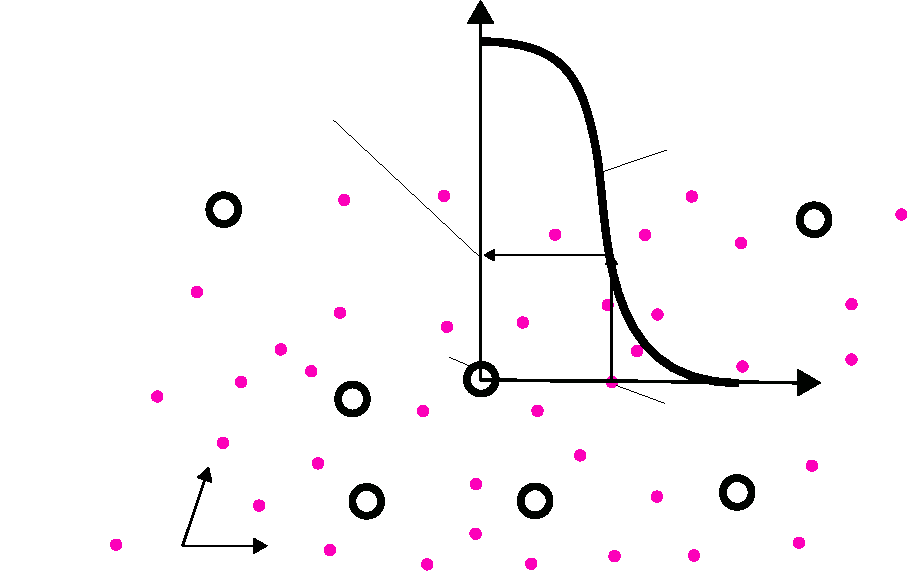
\includegraphics[width=7cm]{Figures/weighs.pdf}
		\caption{2D schematic example of arbitrary weight function of a TPA located with position vector ${\boldsymbol {\rm x}}_{\rm t}$. 
		Points of the discrete field $v({\boldsymbol{\rm x}}_i)$ are presented with dots and points that $v({\boldsymbol{\rm x}}_i)$ is mapped (TPAs) are presented with circles.
		The function is smooth, non-negative, reaches maximum at the TPA and decreases with distance $||{\boldsymbol {\rm x}}_{\rm t} - {\boldsymbol {\rm x}}_i||$. 
		The boundary of the domain of influence of the weight function is presented with dashed ellipsoid (circle on 2D plane) and the function takes a constant value of zero outside of it.}
		\label{fig:weight_func}
	\end{centering}
\end{figure}

Many types of weight functions can be used for MLS method. A one-dimensional quartic spline, commonly used in meshless methods~\citep{belytschko1996meshless}, was chosen for the current work:
\begin{equation}
w(||{\boldsymbol {\rm x}}-{\boldsymbol {\rm x}}_i||/d_{\rm {mi}})=w(r_i)=\begin{cases} 1-6r_i^2+8r_i^3-3r_i^4 & \mathrm{for} \, r_i \leq 1\\ 0 & \mathrm{for} \, r_i > 0 \end{cases}
\end{equation}
Its derivative (required later) with respect to the spatial coordinates is:
\begin{equation}
\frac{dw}{d{\boldsymbol {\rm x}}}= \frac{dw}{dr_i}\frac{dr_i}{d{\boldsymbol {\rm x}}} =\frac{1}{d_{\rm {mi}}}\begin{cases} (-12r_i +24r_i^2 -12 r_i^3) \,  & \mathrm{for} \, r_i \leq 1, \\ 0 & \mathrm{for} \, r_i > 0  \end{cases}
\end{equation}
Here $r_i = ||{\boldsymbol {\rm x}}-{\boldsymbol {\rm x}}_i||/d_{\rm {mi}}$ is the normalised radial distance of point $i$ from the TPA divided by scaling parameter $d_{\rm {mi}}$. 
This coefficient is governing the size of influence domain. 

%The vector of unknowns $\mathbf a({\boldsymbol {\rm x}}_{\rm t}) = \Big[ a_1({\boldsymbol {\rm x}}_{\rm t} ), a_2({\boldsymbol {\rm x}}_{\rm t} ), \dots a_q({\boldsymbol {\rm x}}_{\rm t} ) \Big]$ in Eq.~(\ref{eq:mwls_approx}) can be obtained from a minimization of 
With the above tools at hand, the vector of unknowns $\mathbf a({\boldsymbol {\rm x}}_{\rm t})$ associated to the TPA can be evaluated through minimisation of the weighted discrete $L_2$ norm:
\begin{equation}
J({{\boldsymbol {\rm x}}}_{\rm t})=
\frac{1}{2} \sum_i^{n_{\rm w}} w(r_i) \left( v^h({\boldsymbol {\rm x}}_{\rm t}) - v({\boldsymbol{\rm x}}_i) \right)^2
=
\frac{1}{2} \sum_i^{n_{\rm w}} w(r_i) \left( \mathbf p^{\rm T} ({\boldsymbol {\rm x}}_i)\mathbf a({\boldsymbol {\rm x}}_{\rm t}) - v({\boldsymbol{\rm x}}_i) \right)^2
\label{eq:mwls_l2}
\end{equation}
where $v({\boldsymbol{\rm x}}_i)$ is the value of the given discrete field at point $i$ amongst the $n_{\rm w}$ points located within domain of influence of the TPA and $\mathbf p^{\rm T} ({\boldsymbol {\rm x}}_i)$ is the vector of shape functions of point $i$. 
 
Minimisation of $J$ with respect to $\mathbf a$ leads to a system of linear equations as:
\begin{equation}
\mathbf{ { A }} ({\boldsymbol {\rm x}}_{\rm t}) \mathbf{ { a}} ({\boldsymbol {\rm x}}_{\rm t}) = \mathbf{ { B }}({\boldsymbol {\rm x}}_{\rm t}) \mathbf{ { v}}
\label{eq:mwls_system}
\end{equation} 
where matrices $\mathbf{ { A }}({\boldsymbol {\rm x}}_{\rm {t}})$ and \textbf{$\mathbf{ { B}}({\boldsymbol {\rm x}}_{\rm t})$} are of size $(q \times q )$ and $(q \times n_{\rm w} )$ and defined as follows:
\begin{equation} 
\begin{aligned}
& \mathbf{ { A }}({\boldsymbol {\rm x}}_{\rm t}) = \sum_i^{n_{\rm w}} w (r_i)\mathbf{p} ( {\boldsymbol {\rm x}}_i)\mathbf p^{\rm T} ({\boldsymbol {\rm x}}_i) \\
& \mathbf{ { B }}({\boldsymbol {\rm x}}_{\rm t}) = \Big[   w(r_1) \mathbf p ({\boldsymbol {\rm x}}_1), w(r_2) \mathbf p ({\boldsymbol {\rm x}}_2), \dots ,  w(r_{n_{\rm w}}) \mathbf p ({\boldsymbol {\rm x}}_{n_{\rm w}})  \Big]
\end{aligned}
\end{equation}
and $\mathbf v$ is $(n_{\rm w} \times 1)$ vector of the given field values at the points within the influence domain given as: 
\begin{equation}
\mathbf v = \big[ v({\boldsymbol {\rm x}}_{\rm 1}), v({\boldsymbol {\rm x}}_{\rm 2}), \dots, v({\boldsymbol {\rm x}}_{n_{\rm w}}) \big]^{\rm T}
\end{equation}
It should be noted that parameter $d_{\rm{mi}}$ is chosen to include sufficient $n_{\rm w}$~points such that the resulting matrix $\boldsymbol {\rm A}$ is not singular. 
Next, Eq.~(\ref{eq:mwls_approx}) combined with Eq.~(\ref{eq:mwls_system}) can be rewritten as: 
\begin{equation}
v^h({\boldsymbol {\rm x}}_{\rm t} )= \sum^{n_{\rm w}}_{i=1} \omega_i({\boldsymbol {\rm x}}_i) v_i = \mathbf {\bm {\upomega}}^{\rm T} ({\boldsymbol {\rm x}}_{\rm t}) \mathbf v 
\end{equation}
where $ {\boldsymbol {\rm {\upomega}}} ({\boldsymbol {\rm x}}_{\rm t})$ is a resulting vector of shape functions associated with the TPA, defined as
\begin{equation}
{\boldsymbol \upomega}^{\rm T} ({\boldsymbol {\rm x}}_{\rm t}) = \mathbf p^{\rm T} ({\boldsymbol {\rm x}}_{\rm t}) \mathbf{A}^{-1} ({\boldsymbol {\rm x}}_{\rm t}) \mathbf B ({\boldsymbol {\rm x}}_{\rm t})
\end{equation}
It is also necessary to approximate the density's spatial gradient
Therefore, the first derivative of the shape function with respect to the spatial coordinates is derived in direction $x_j$:
\begin{equation}
{\boldsymbol {\upomega}}^{\rm T}_{,j} = \mathbf p^{\rm T}_{,j} \mathbf A^{-1} \mathbf B + \mathbf p^{\rm T} ( \mathbf A_{,j}^{-1} \mathbf B + \mathbf A^{-1} \mathbf B_{,j} )
\end{equation}
The commas in the subscripts denote the partial derivative and the inverse of the spatial derivative of matrix $\boldsymbol {\rm A}$ is evaluated as 
\begin{equation}
\mathbf A_{,j}^{-1} = -\mathbf A^{-1} \mathbf A_{,j} \mathbf A^{-1}
\end{equation}
It is worth noting that for any TPA located at ${\boldsymbol {\rm x}}_{\beta}$, MLS shape functions do not satisfy Kronecker delta function, i.e. $\omega_i({\boldsymbol {\rm x}}_{\beta}) \neq \delta_{i\beta}$. 
%The values obtained from the MLS approximation are not the same as the given field values, i.e. $v^h({\boldsymbol {\rm x}}_{\beta}) \neq v({\boldsymbol {\rm x}}_{\beta}) $ as presented with a 1D example in Figure~\ref{fig:mwls_approxi}.
%\begin{figure}[h!]
%	\begin{centering}
%		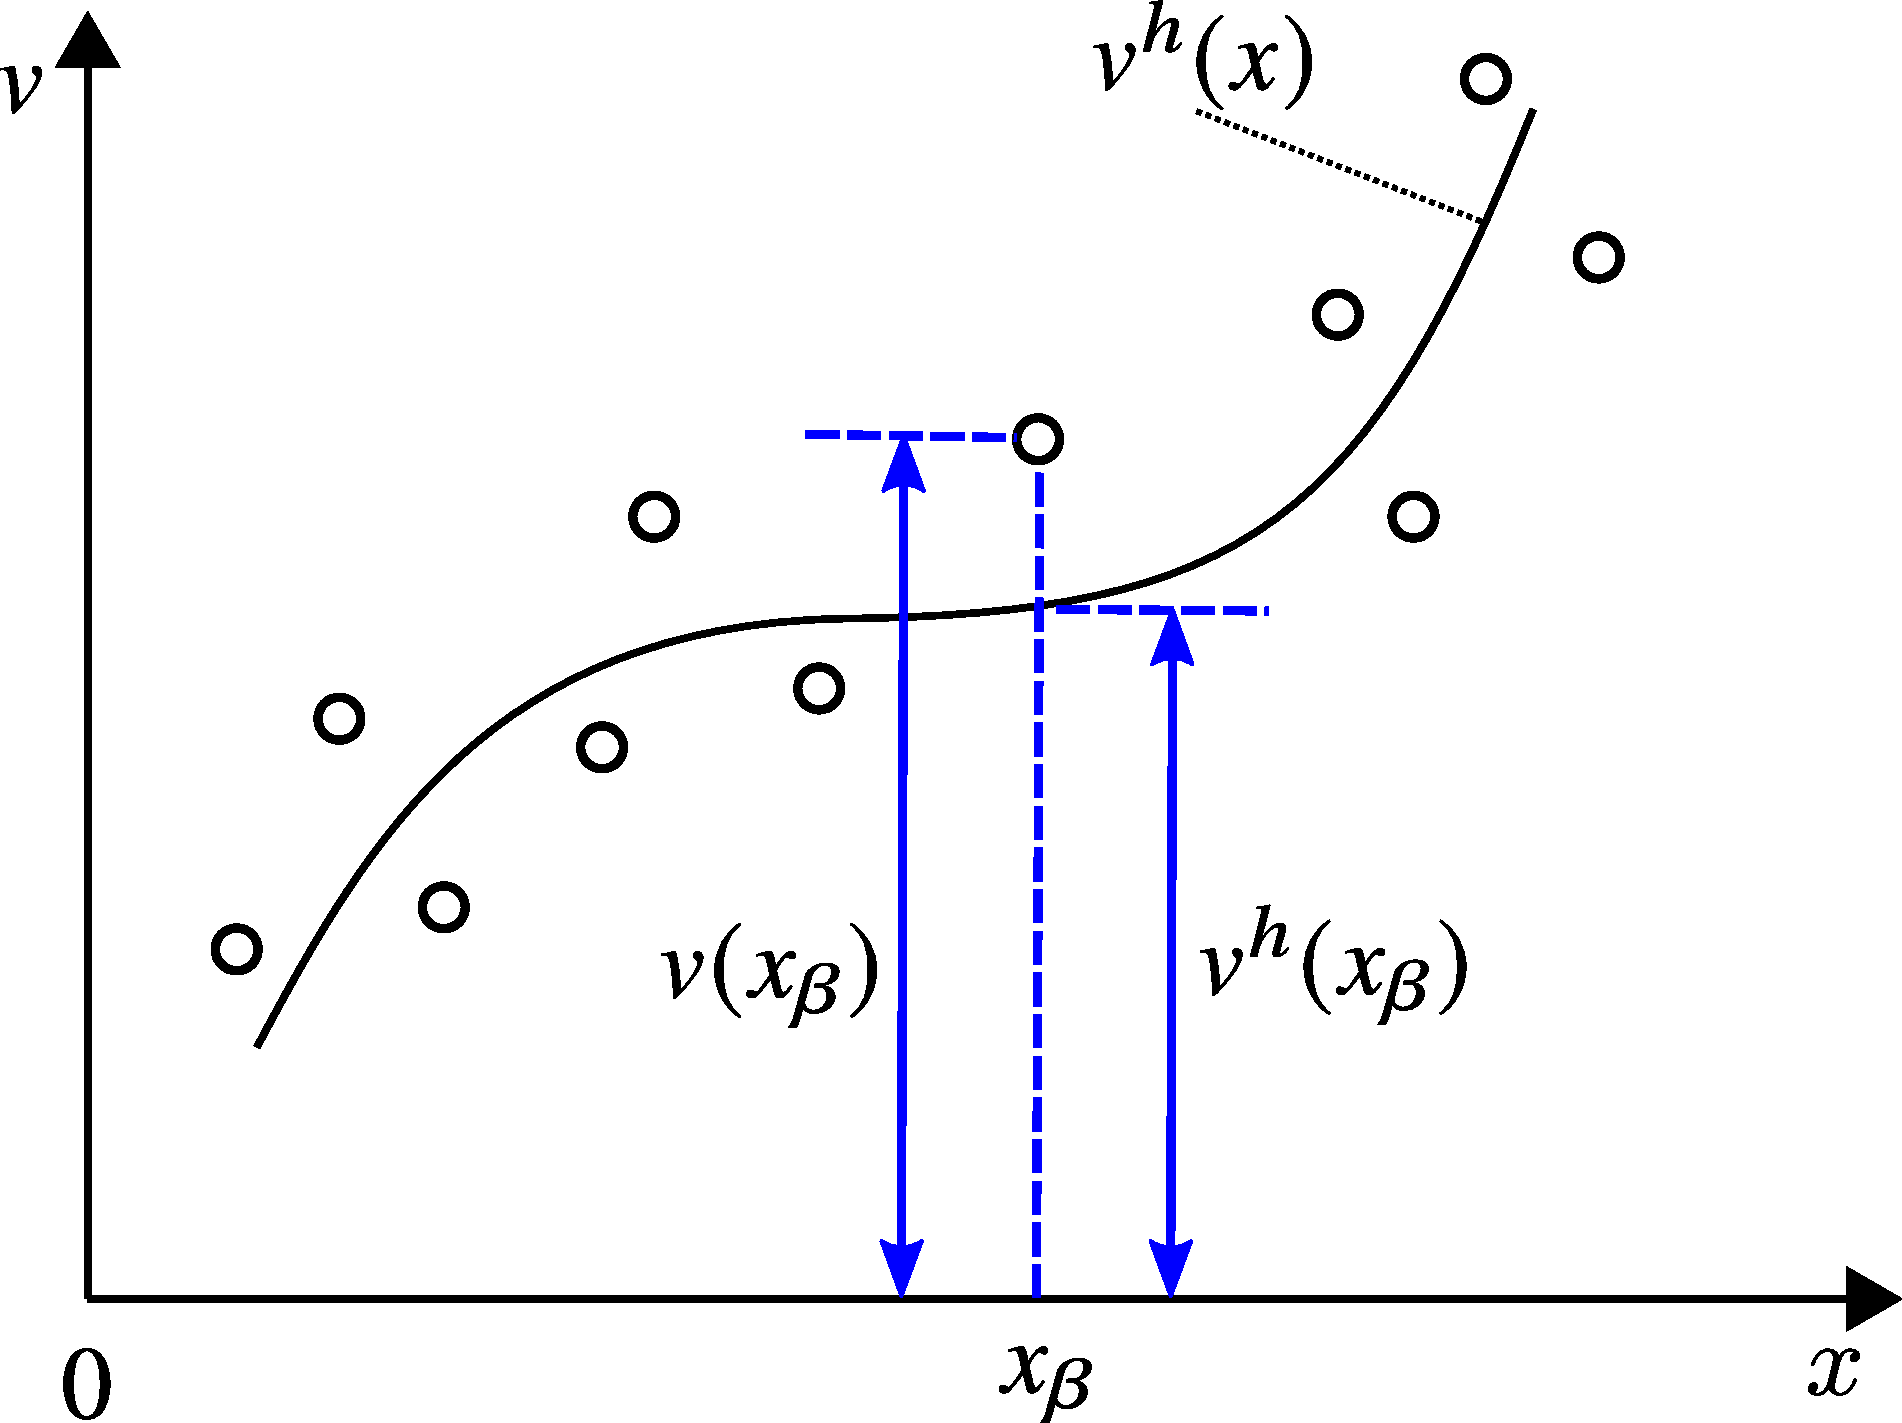
\includegraphics[width=7cm]{Figures/1dMWLS.pdf}
%		\caption{1D example of moving least squares method.}
%		\label{fig:mwls_approxi}
%	\end{centering}
%\end{figure}
%Since the MLS shape functions do not satisfy Kronecker-delta property on the boundaries of the problem; it can be quite a challenge to enforce essential boundary conditions, however, here approximation is used for simple mapping hence this problem can be neglected. 
\\

A common problem arising from CT scanning is generation of Partial Volume Artifacts~\citep{adams2009quantitative}. As a result, the voxel data can be averaged between two materials, for example bone and soft tissue.
To eliminate mapping spurious bone densities, some researchers have proposed to either redefine data at any node on the mesh surface to data assigned on the nearest internal node~\citep{helgason2008modified, chen2010new} or resurface the mesh geometry~\citep{peleg2014can}. 
In this study, a more elegant solution is proposed; every CT scan data point positioned outside the geometry of the bone is simply removed from the domain of influence, thereby only points that fall inside the volume are approximated. 
%Determining whether a given point is inside a polyhedron is a classic computer graphics problem.  It can be solved by casting a ray originating from the given point to an arbitrary direction and determine the number of intersections of the ray with the polyhedron. If the ray intersects the shape an even number of times, then the point is outside the shape. It is important to choose a random direction. (should I describe why based on measure theory?) In MoFEM implementation standard C++ $rand()$ function was used, however without the seed in order to ensure that the code remains deterministic. 
This procedure only has to be performed once for each domain of influence  and can be easily parallelized. %is 'embarrasingly parrallel' 

\section{Fracture risk following bone adaptation}\label{sec:release_energy}
Various theories exist in the literature regarding failure criteria for bone tissue and it is now common practice for researchers to estimate fracture risk within the framework of FEM. In particular, subject-specific FEM models can potentially quantify the risk of failure under a given loading scenario. However, this still remains an open challenge.

In recent years, the main focus in bone mechanics was in the use of different strength criteria for onset of failure. 
The most commonly adopted ones were based on stress~\citep{keyak2005predicting} or strain measures~\citep{schileo2008subject} assuming the bone failure under the von Mises, the Drucker-Prager or maximum principal strain and maximum principal stress yield criterion~\citep{yosibash2010predicting}. 
The experimental validations for such simplified models show that they have a significant spread in the predicted failure. 
The percentage error in the majority of studies report is between 10\% and 20\%~\citep{van2014accurately}.

This variation is explained perhaps by their focus on the local initiation of failure, rather than the complete failure mechanism. 
The fracture process of bone is very important,  particularly in the case of fatigue fractures~\citep{gupta2008fracture}. 
Limitations in previous studies (e.g. use of 2D geometry~\citep{bettamer2017using}, assuming homogeneous bone properties~\citep{gasser2007numerical}), 
can also explain why an appropriate model for bone fracture has not been developed previously.

There are many methods available to numerically simulate fracture initiation and growth. 
They can be divided into two categories: discrete and smeared approaches. 
Discrete crack models originally were limited to describe crack formation only on element boundaries~\citep{Scordelis1967}. 
More recently, in the presence of automatic mesh generators, the extended finite element method (xFEM) separated the crack path from underlying mesh, see e.g.~\citep{Belytschko1999} where xFEM was applied to model brittle fracture. 
Lattice element approach (also known as rigid body spring networks) have also been used to model discrete crack paths for concrete at computational low cost~\citep{bolanderSaito1998, grassl2010}.  
Another novel approach in isogeometric analysis that introduces knot insertions that lower the order of continuity to introduce cracks in solids~\citep{Hosseini2014}. 
The continuum damage, or diffused crack approach, incorporates a damage parameter into the model that controls the strength of the material. An advantage of this approach is that it does not require interface tracking since the damage parameter varies continuously over the domain (see, e.g.~\citep{deBorst2004}). 
Closely related to continuum damage models are the phase-field models which have become extremely popular over the last decade. 
The numerical solution of these models is based on an approximate potential developed by Mumford~\citep{Mumford1989}. 
The main advantage is that the fracture problem can be described purely by partial differential equations~\citep{Miehe2010a,Borst2014}. \\

This paper presents a modified formulation and associated computational framework for brittle fracture in elastic solids within the context of configurational mechanics in heterogeneous materials like bones, extending the authors' previous work~\citep{kaczmarczyk2017energy}. 
Configurational mechanics utilises the concept of material (configurational) forces originally introduced by Eshelby~\citep{eshelby1951force}. 
Unlike physical forces, material forces act on the material manifold and represent the tendency of imperfections like cracks, voids or material inhomogeneities to move relative to the surrounding material. 
The past two decades have seen a growing interest in this approach for analysis of material imperfections~\citep{maugin2016configurational} and in particular for evaluation of crack-driving forces~\citep{steinmann2001application, ozencc2016configurational, kaczmarczyk2017energy}. 
Such implementations in the framework of Finite Element analysis have proven to be accurate, robust and capable of handling a propagation of complex 3D non-planar crack surfaces. However, until recently the approach have never been used to effectively assess material forces in a heterogeneous bodies with cracks. 
For this purpose, in the current study, additional material forces arising from inhomogeneities are introduced into the formulation. Such modification allows for identification of the liability of an arbitrary crack to propagate and in the future can be extended to simulate full fracture propagation in bone. 
An additional goal is to investigate bone failure at different stages of bone adaptation, utilising the results from bone remodelling analysis or data directly taken from CT scans. 
Similar concept of combined remodelling and fracture analyses has been presented before~\citep{hambli2013integrated}. 
However, it utilised a different remodelling model and continuum damage mechanics approach for fracture, both of which require many more parameters to calibrate. 
\subsection{Kinematics}\label{sec:Kinematics}
In the context of configurational mechanics, an elastic body with an initial crack, as visualised in Figure~\ref{fig:frac_kinematics}, is considered. 
To independently observe the deformation of the material in physical space $\Omega_t$ and the evolution of the crack surface in material space $\mathcal B_t$ it is convenient to decompose the problem into separate configurations. 
First, propagation of the crack is described by the mapping from the reference configuration to the current material domain, $\Xi$. Next, purely elastic deformation is mapped from the current material to spatial domain, $\mathbf \varphi$. 
Let $\mathbf x = \varphi(\mathbf X,t)$ describe the motion of the body, which transforms material positions, $\mathbf X$, to their spatial counterparts, $\mathbf x$. 
The physical displacements are derived as follows:
\begin{equation}
\mathbf u = \mathbf x - \mathbf X
\end{equation}
The reference configuration represents the body before crack extensions with mapping $\mathbf \Xi( { \boldsymbol {\rm \upchi}}, t)$ of the reference coordinates, ${ \boldsymbol {\rm \upchi}}$, on to the material coordinates, $\mathbf X$. 
This mapping describes a material structural change like extensions of the crack as a result of the crack front movement. 
\begin{figure}[h!]
	\begin{centering}
	%	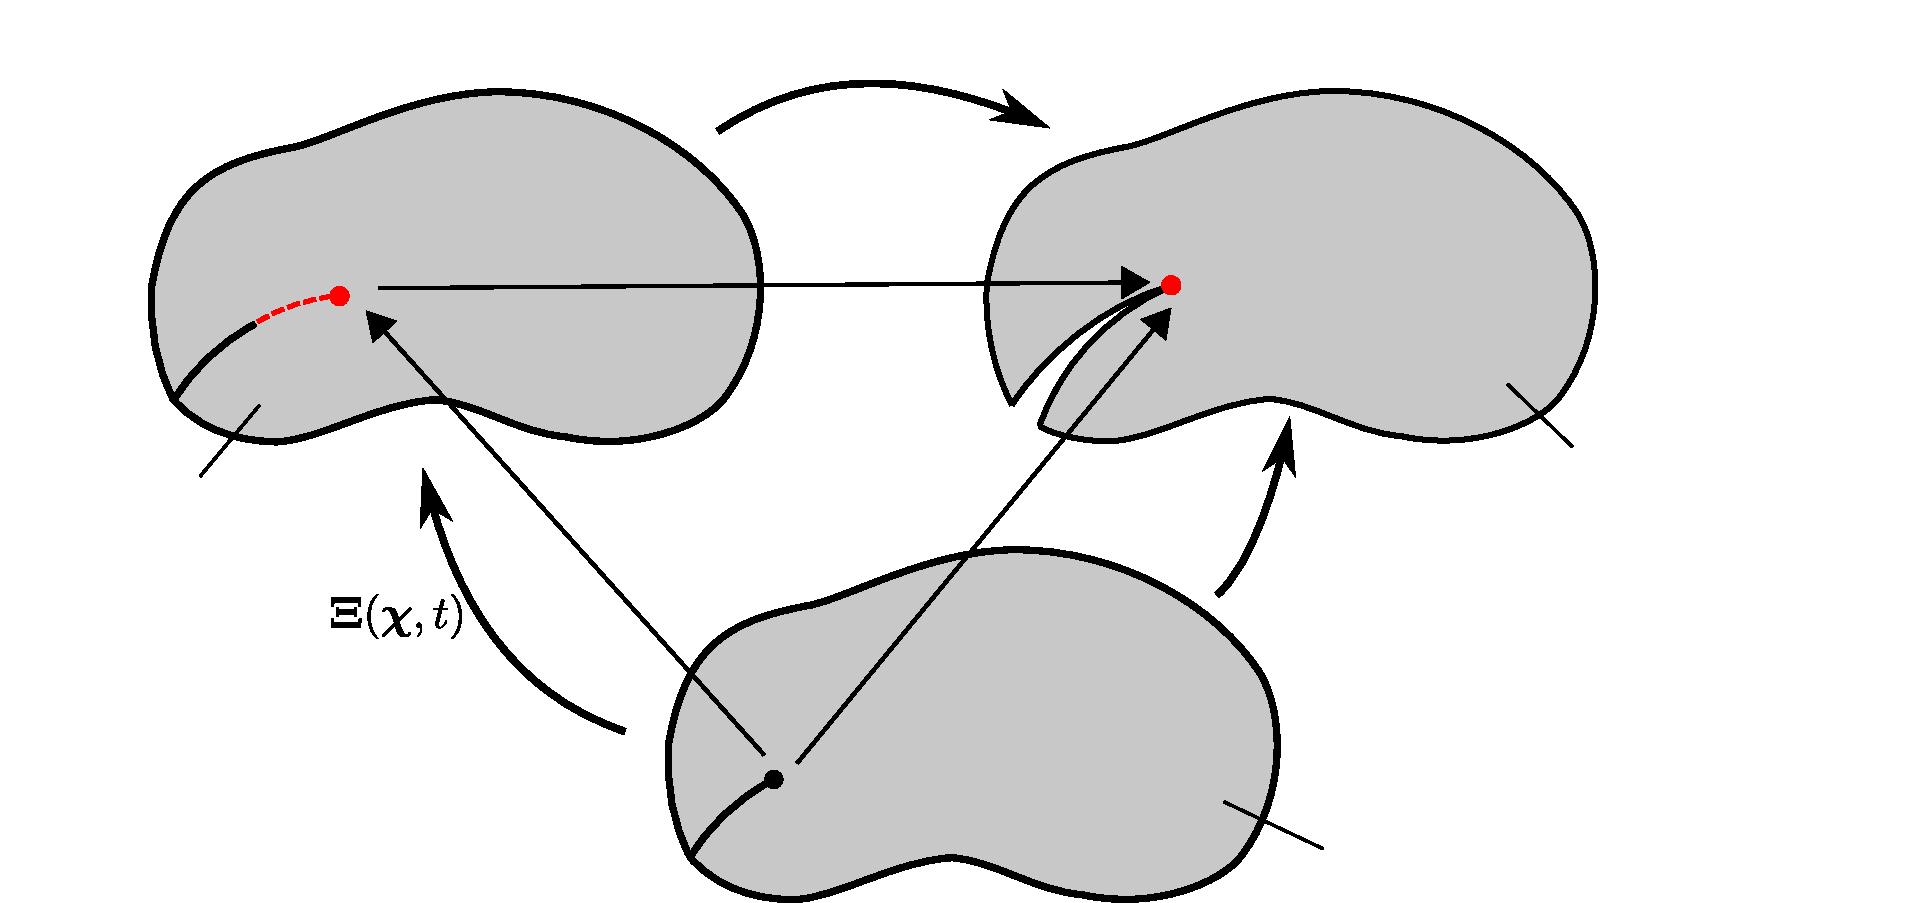
\includegraphics[width=10cm]{Figures/Configurations.pdf}
	\def\svgwidth{10cm}
	\input{Figures/Configurations.pdf_tex}
		\caption{Decomposition of crack propagation in an elastically deforming body.}
		\label{fig:frac_kinematics}
	\end{centering}
\end{figure}
Finally, mapping $\mathbf \Phi ({ \boldsymbol {\rm \upchi}},t)$ transforms reference coordinates on to the spatial coordinates, ${\boldsymbol {\rm x}}$. The current material and spatial displacements are:
\begin{equation}
\mathbf W = \mathbf X - { \boldsymbol {\rm \upchi}} \quad \mathrm{and} \quad \mathbf w = \mathbf x - { \boldsymbol {\rm \upchi}}
\end{equation}
$\mathbf H$ and $\mathbf h$  gradients of the material and spatial maps are defined as:
\begin{equation}
\mathbf H = \nabla_{\boldsymbol {\rm \upchi}} {\boldsymbol {\rm \Xi}}, \quad \mathbf  h =   \nabla_{\boldsymbol {\rm \upchi}} {\boldsymbol {\rm \Phi}}
\end{equation}
Corresponding deformation gradient $\mathbf F$ is derived as follows:
\begin{equation}
\mathbf F = \nabla_{ \boldsymbol {\rm \upchi}} \varphi=\mathbf h \mathbf H^{-1}
\end{equation}
Since physical material cannot penetrate itself or reverse the orientation of material coordinates, the following constraint has to be imposed:
\begin{equation}
{\mathrm {det}} \mathbf {F} = \frac{\mathrm {det} (\mathbf h)}{\mathrm {det} (\mathbf H)} > 0
\end{equation}
Moving on, the velocity of a material point $\mathbf X$ and the time derivative of the deformation gradient have the following form:
\begin{equation}\label{eq:crack_disp}
{\dot {\boldsymbol {\rm u} } } = {\dot {\boldsymbol {\rm w} } } - \mathbf F{\dot {\boldsymbol {\rm W} } }
\end{equation}
and
\begin{equation}\label{eq:crack_def_grad}
{\dot {\boldsymbol {\rm F} } } = \nabla_{\mathbf X} {\dot {\boldsymbol {\rm w} } } - \mathbf F \nabla_{\mathbf X } {\dot {\boldsymbol {\rm W} } }
\end{equation}
\begin{figure}
	\begin{centering}
	%	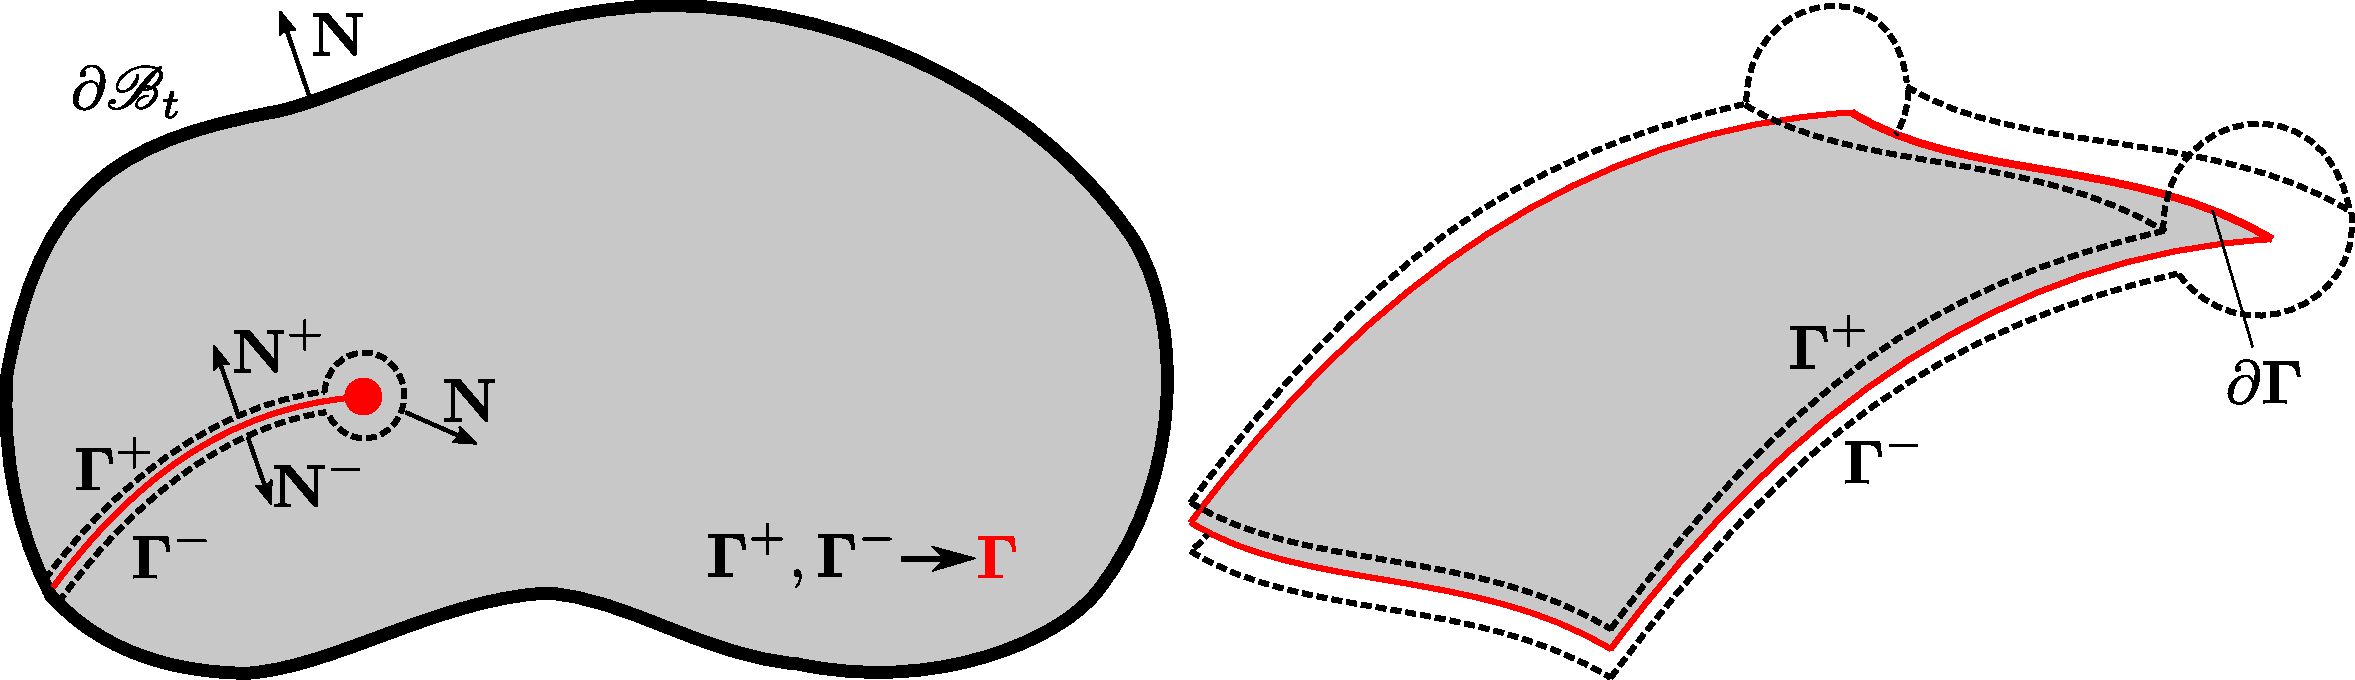
\includegraphics[width=12cm]{Figures/CrackSurface.pdf}
		\def\svgwidth{12cm}
		\input{Figures/CrackSurface.pdf_tex}
		\caption{Crack construction~\citep{kaczmarczyk2017energy}.}
		\label{fig:frac_crack_con}
	\end{centering}
\end{figure}
\subsection{Crack front}
The crack surface is denoted as $\Gamma$ with a crack front $\partial \Gamma$, see Figure~\ref{fig:frac_crack_con}.  Following~\citep{kaczmarczyk2014three}, a kinematic relationship between the change in crack surface area $\dot A_\Gamma$ and the crack front velocity $\mathbf{\dot W}$ can be defined as:
\begin{equation}\label{eq:crack_front}
\dot A_\Gamma = \int_{\partial \Gamma} \mathbf A_{\partial \Gamma} \cdot {\dot {\boldsymbol {\rm W} } } \mathrm d L 
\end{equation}
where $ \mathbf A_{\partial \Gamma}$ is a kinematic state variable that defines the current crack front orientation. It should be noted that any change in the crack surface area $\dot A_\Gamma $ and the crack front velocity $\mathbf {\dot W}$ in the material configuration can only take place when the crack propagates. 
%\begin{equation}
%\mathbf \Xi : \mathcal B_0 \to \mathcal B_t, \quad \mathbf X = \mathbf \Xi(\mathbf \upchi, t)
%\end{equation}
\subsection{Dissipation of energy at the crack front}
Crack propagation problem can be considered as a thermodynamic system consisting of a solid deformable body with an imperfection. 
Traction applied on the boundary of the body $\partial \mathcal B_t$ performs work on the system. 
Following the first law of thermodynamics, it can be assumed that all energy within the volume of the body is used for mechanical work and it can be expressed as 
\begin{equation}
\int_{\partial \mathcal B_t} {\dot {\boldsymbol {\rm u} } } \cdot \mathbf t \mathrm d S = \gamma \dot A_\Gamma +{\frac{\mathrm d}{\mathrm d t }} \int_{\mathcal B_t} \Psi(\mathbf F) \mathrm d V
\end{equation}
where the left hand side is the power of external work. 
The first term on the right hand side is the rate of the crack surface energy and the last term is the rate of internal body energy. 
Furthermore, $\mathbf t$ is the external traction vector, $\gamma $ is the surface energy $[ {\rm{N m}}^{-1} ]$ and $\Psi$ is the free energy density function. 
Next, by substituting Equations (\ref{eq:crack_disp}),(\ref{eq:crack_def_grad}) and (\ref{eq:crack_front}) and given that $\mathrm d \dot V = \nabla _{\mathbf X} \cdot \mathbf{\dot W} \mathrm d V$, the above expression can be reformulated as:
\begin{equation}\label{eq:crack_first_law}
\int_{\partial \mathcal B_t} \big( {\dot {\boldsymbol {\rm w} } } \cdot \mathbf t - {\dot {\boldsymbol {\rm W} } } \cdot \mathbf F^{\rm T} \mathbf t \big) \mathrm d S = \int_{\partial \Gamma } \gamma \mathbf A_{\partial \Gamma} \cdot {\dot {\boldsymbol {\rm W} } } \mathrm d L + \int_{\mathcal B_t} \big( \mathbf P\, \colon \nabla_{\mathbf X} {\dot {\boldsymbol {\rm w} } } + {\bm  \Sigma}\, \colon \nabla_{\mathbf X} {\dot {\boldsymbol {\rm W} } } \big) \mathrm d V 
\end{equation}
where
\begin{equation}
\mathbf P = \frac{\partial \Psi (\mathbf F, \rho)}{\partial \mathbf F} \quad \mathrm{and } \quad {\bm {\Sigma}} = \Psi(\mathbf F) \mathbf  1 - \mathbf F^{\rm T} \mathbf P
\end{equation}
are the first Piola-Kirchhoff stress and Eshelby stress tensors, respectively. 
The former quantity is a well-known driving force for elastic deformation in the spatial domain. 
It is worth noting that $\boldsymbol{\rm P}$ previously presented for bone material model in Subsection~\ref{sec:constitutive_eq}, also depends on density, $\rho$. 
The Eshelby stress is Piola's material counterpart and is the driving force for local configurational changes in the material domain. 
Local form of the first law in Eq.~(\ref{eq:crack_first_law}) can be obtained by applying the divergence theorem to the last integral in Eq.~(\ref{eq:crack_first_law}) resulting in the following expression:
\begin{equation}\label{eq:crack_local_gauss}
\begin{aligned}
&  \int_{\partial \Gamma } \gamma \mathbf A_{\partial \Gamma} \cdot {\dot {\boldsymbol {\rm W} } } \mathrm d L = \int_{\mathcal B_t} {\dot {\boldsymbol {\rm w} } } \cdot \big( \nabla_{\mathbf x} \cdot \mathbf P  \big) \mathrm d V + \int_{\mathcal B_t} {\dot {\boldsymbol {\rm W} } } \cdot \big( \nabla_{\mathbf x} \cdot {\bm {\Sigma}} \big) \mathrm d V \\
& +\int_{\partial \mathcal B_t \cup \Gamma^+ \cup \Gamma^-} {\dot {\boldsymbol {\rm w} } }\cdot \big( \mathbf t - \mathbf{PN}\big) \mathrm  d S + \int_{\partial \mathcal B_t \cup \Gamma^+ \cup \Gamma^-}  {\dot {\boldsymbol {\rm W} } } \cdot \big( \mathbf F^{\rm T} + {\bm {\Sigma}} \mathbf{ N} \big) \mathrm d S \\
& - \lim_{\mathcal C \to 0} \int_{\mathcal C} {\dot {\boldsymbol {\rm w} } } \cdot \mathbf {PN} \mathrm d S + \lim_{\mathcal C \to 0} \int_{\mathcal C} {\dot {\boldsymbol {\rm W} } } \cdot {\bm {\Sigma}}\mathbf{N} \mathrm d S
\end{aligned}
\end{equation}
Moreover, it can be recognised that, in the limit, the surface $\mathcal C$ (Figure~\ref{fig:frac_crack_con}) collapses to the crack front $\partial \Gamma $ and integrals over the crack front are simplified as follows:
\begin{equation}
\lim_{\mathcal C \to 0} \int_{\mathcal C} (\cdot ) \mathrm d S = \lim_{\mathcal C \to 0} \int_{\mathcal L_t} \int_{\mathcal L_n} (\cdot) \mathrm d S = \int_{\partial \Gamma} \lim_{|\mathcal{ L }|\to 0} \int_{\mathcal L_n } (\cdot ) \mathrm d S
\end{equation}
The spatial conservation law of linear momentum balance, for any point inside the body, is expressed as follows:
\begin{equation}
\nabla_{\mathbf X} \cdot \mathbf P = 0
\end{equation}
Therefore, the first term on the right-hand side in Eq.~(\ref{eq:crack_local_gauss}) vanishes. 
However, the material conservation law is not equal to zero in case of heterogeneous materials like bones. 
Following~\citep{kienzler2014configurational}, material defects and inhomogeneities can create additional configurational forces; hence, material momentum balance can be expressed as:
\begin{equation}
\nabla_{\mathbf X } \cdot {\bm {\Sigma}}= \mathbf f^{\mathrm {inh}}
\end{equation}
where $ \mathbf f^{\mathrm {inh}}$ is a fictitious force, directed from the $ \textit {harder}$ part of the material to the $ \textit {softer}$ part. 
It represents a vector of the spatial variation of material properties, and in the context of heterogeneous bodies considered in this study it has the following form:
\begin{equation}
\mathbf f^{\mathrm {inh}} = -\left. \left( \frac{\partial \Psi }{ \partial \mathbf X} \right) \right|_{\mathbf x= \mathrm{const}} = - \left. \left( \frac{\partial \Psi}{\partial \rho} \right) \left( \frac{\partial \rho}{\partial \mathbf X} \right) \right|_{\mathbf x= \mathrm{const}}
\end{equation}
where $\Psi$ is the free energy that depends on density as noted in Eq.~(\ref{eq:free_energ}). 
Above expression is an explicit derivative - it does not depend on the spatial configuration $\mathbf x$.

Furthermore, considering only admissible velocity fields and stress fields in equilibrium with external forces, the following expression can be obtained. 
\begin{equation}
\int_{\partial \Gamma } \gamma \mathbf A_{\partial \Gamma} \cdot {\dot {\boldsymbol {\rm W} } } \mathrm d L -\int_{\partial \Gamma} {\dot {\boldsymbol {\rm W} } } \cdot \lim_{|\mathcal L_n| \to 0 }  \int_{\mathcal L_n } {\bm {\Sigma}}\mathbf{N} \mathrm d S  = 0
\end{equation}
The configurational (material) force at the crack front, which is the material counterpart of the spatial internal force vector is defined as:
\begin{equation}
\mathbf G = \lim_{|\mathcal{ L }|\to 0} \int_{\mathcal L_n} {\bm {\Sigma}}\mathbf{N}\, \mathrm d L 
\label{eq:crack_configuration_force}
\end{equation}
It should be noted that for a continuous and homogeneous elastic body, the material force $\mathbf G$ away from the crack should be zero.
Next, the local form of the first law presented in Eq.~(\ref{eq:crack_local_gauss}) is: 
\begin{equation}\label{eq:crack_local_first_law}
{\dot {\boldsymbol {\rm W} } } \cdot \left( \gamma \mathbf A_{\partial \Gamma} - \mathbf G \right) = 0
\end{equation}
This equation represents the equilibrium condition for the crack front. 
The term $ \gamma \mathbf A_{ \partial \Gamma }$ can be considered as material resistance. However, the crack evolution is not within the scope of this study. \\
\subsection{Spatial and material discretisation}
\textcolor{red}{This section will be corrected by Lukasz.} \\
The finite element approximation is applied to both the material and physical space:
\begin{equation}
\begin{aligned}
& \mathbf{ X^h} = \mathbf \Phi({\boldsymbol {\rm {\upchi}}}) \tilde {\mathbf{ X}}, \quad \mathbf{x^h} = \mathbf{\Phi}({\boldsymbol {\upchi}}) {\tilde{\mathbf{x}}} \\
& \mathbf{ W^h} = \mathbf \Phi(\upchi) {\dot { \tilde {\boldsymbol {\rm W} } }}, \quad \mathbf{w^h} = \mathbf{\Phi}({\boldsymbol {\upchi}}){\dot { \tilde {\boldsymbol {\rm w} } }}
\end{aligned}
\end{equation}
where superscript h indicates approximation and $(\tilde \cdot)$ nodal values. 
Three-dimensional domains are discretised with tetrahedral finite elements with hierarchical basis functions of arbitrary polynomial order, following the work of Ainsworth and Coyle~\citep{Ainsworth2003}. 
The higher-order approximations are only applied for displacements in the spatial configuration, whereas a linear approximation is used for displacements in the material space. 
The material and spatial gradients of deformation are expressed as:
\begin{equation}
\mathbf H^h = \mathbf{B_x}(\upchi) {\tilde{\mathbf{X}}}, \quad \mathbf h^h = \mathbf{B_x} ({\boldsymbol {\upchi}}) { \tilde{\mathbf{x}}}, \quad \mathbf F^h = \mathbf h^h (\mathbf H^h)^{-1} = \mathbf{B_x} \mathbf{\tilde x}
\end{equation}
The residual force vector in spatial domain has the classical form:
\begin{equation}
\mathbf r_s^h = \mathbf f_\mathrm{{ext,s}}^h - \mathbf f_\mathrm{{int,s}}^h
\end{equation}
where $\mathbf f_\mathrm{{ext,s}}^h $ and $  \mathbf f_\mathrm{{int,s}}^h$ are the vectors of internal and external forces, respectively, and take the following format:
\begin{equation}
\mathbf f_\mathrm{{ext,s}}^h = \aoperator_{\text{TRI}}^{n_{\rm {el}}} \int_\text{TRI} \mathbf \Phi^{\rm T} \mathbf t^h \mathrm d S, \quad \mathbf f_\mathrm{{int,s}}^h = \aoperator_{\text{TET}}^{n_{\rm {el}}} \int_\text{TET}  (\mathbf{ B_x})^{\rm T} \mathbf{P}^h \mathrm d V
\end{equation}
Therein, the operator $ \aoperator$ symbolises the assembly of all contributions for tetrahedral and triangular elements. The discretised version of Eq.~(\ref{eq:crack_configuration_force}) renders the residual force vector in the material domain, expressed as:
\begin{equation}
\mathbf r_m^h = \mathbf f^h_{\text{res}} - \mathbf{\tilde G}^h
\end{equation}
The nodal material forces $\mathbf{\tilde G}^h$ are the driving force for the crack front propagation and have the following form:
\begin{equation}\label{eq:crack_material_force_dis}
\mathbf{\tilde G}^h = \aoperator_{\text{TET}}^{n_{\rm {el}}} \int_\text{TET} (\mathbf{B_x})^{\rm T} {\bm {\Sigma}}^h +   \left.\left( \frac{\partial \Psi}{\partial \rho} \right)\right|_{\mathbf{x}= \text {const}} \mathbf{B_x}^{\rm T} \rho \mathrm \,d V
\end{equation}
The explicit derivative of energy with respect to density in Eq.~(\ref{eq:crack_material_force_dis}) is derived automatically by means of ADOL-C library~\citep{Walther2009}. 
Furthermore, $\mathbf f^h_{\text {res}}$ is the vector of nodal material resistance (Griffith) forces, given as:
\begin{equation}
\mathbf f^h_{\text{res}} = \frac{1}{2} (\mathbf{\tilde A}^h_\Gamma)^{\rm T} \mathbf g_c
\end{equation}
where $ \mathbf g_c$ is a vector with zero for all components except those associated with nodes on the crack front, where the value is equal to $g_c$. 
It is a material parameter specifying the critical threshold of energy release per unit area of the crack surface $\Gamma$, also known as the Griffith energy.

\section{Numerical examples}
\label{sec:numerical_examples}
In this section, several numerical examples are presented to illustrate each aspect of the proposed framework. 
The first set of analyses, presented in Subsection~\ref{sec:numerical_examples:bone_adap}, considers the bone adaptation of an equine 3rd metacarpal bone. 
The second set of analyses, in Subsection~\ref{sec:mals_mapping}, show the results of MLS mapping onto an FE mesh. 
Concept of quarter point elements is demonstrated in Subsection~\ref{sec:release_energy_rate} used to produce stress singularity at crack tip.
In the same subsection, implementation is verified for numerical finite plate with through thickness crack subjected to uniaxial stress where model results are compared with analytical solution for infinite plate. 
For the same example, convergence study is conducted for standard and quarter point elements.
Finally, the framework is validated through analysis of metacarpal bone where release energy rate is computed at different remodelling stages.

%Finally, the results of release energy rate for simple finite plate problem and metacarpal bone are presented in Subsection~\ref{sec:release_energy_rate} verifying the implementation. 
%Additionally, convergence study is conducted with and without quarter point elements at the crack tip.
\subsection{Bone adaptation examples}
\label{sec:numerical_examples:bone_adap}
This subsection considers the bone adaptation of an equine 3rd metacarpal bone.
Three cases are studied where they all have the same material parameters presented in Table~\ref{tab:parameters_mc3}.
The values are adopted based on previous studies of human tibia~\citep{Pang2012,Waffenschmidt2012}. 
Higher stiffness of equine bones, derived from mechanical testing studies~\citep{Les1994}, is also taken into account.

Each case considers a different function for the parameter $c$ that defines the rate of bone remodelling and used to compute the mass source, $\mathcal{R}_0$, according to Eq.~(\ref{eq:mass_source}).
In Case~1, $c$ is constant. For Case~2 and Case~3 different bell functions (Eq.~(\ref{eq:bell_function}) are used. The parameters for each case are presented in Table~\ref{tab:three_cases}. 
The FE mesh used in all cases comprises 17041 tetrahedral elements and was generated by discretising the segmented geometry of a full-scale model of equine 3rd metacarpal bone derived from CT scan data - see Figure~\ref{fig:mc3_BC}.

For each analysis, the initial density is chosen to be homogeneous since, in the thermodynamic-based model, the starting density does not have a significant effect on the final bone density distribution (similar to other models at biological equilibrium~\citep{kuhl2003theory}). % is not sensitive to the initial density
Boundary conditions are simplified to two representative forces (5~$\text{[kN]}$~each) spanning over a small area based on pressure film studies~\citep{Brama2001}, as demonstrated in Figure~\ref{fig:mc3_BC}. 
The two forces are often considered in the literature as an equivalent of joint peak force at the mid-stance of a horse gait. %Obviously, with such simplified loading case the analysis is not sufficient to produce any quantitative results regarding remodelling of the metacarpal but rather to demonstrate the potential of this approach. 
An adaptive time stepping scheme, provided by the PETSc package~\citep{petsc-web}, is used in all the simulations with an initial time step $\Delta t = 0.5$~$[\text d]$, maximum time step of $\Delta t_{\text {max}} = 50$~$[\text d]$ and minimum of $\Delta t_{\text {min}} = 0.05$~$[\text d]$.
\begin{table}[h]
	\centering
	\begin{tabular}{lll}
		\hline
		Parameter             & Description                  & Value  \\ \hline
		$E  $                 & Young's modulus              & $4700 \,\mathrm{ [MPa]}$ ~\citep{Les1994} \\
		$\nu  $               & Poisson ratio                & $0.3 \,\mathrm{ [-]}$ \\
		$\rho_0 ^\ast  $      & Initial density              & $1.0 \,\mathrm{[ g/cm^{3}]}$  \\
		$\psi_{0}^\ast $      & Target energy densidy        & $0.0275\,\mathrm{ [MPa]}$  ~\citep{Waffenschmidt2012}  \\
		$c$                   & Density growth velocity      & $1.0 \,\mathrm{ [d/cm^{2}]}$   \\
		$m$                   & Algorithmic exponent         & $ 3.25 \,\mathrm{ [-]}$          \\
		$n$                   & Porosity exponent            & $2.25 \,\mathrm{ [-]}$     ~\citep{Les1994}   \\ 
		\hline
	\end{tabular} 
	\caption{Material parameters used for the simulations of 3rd metacarpal bone remodelling.}
	\label{tab:parameters_mc3}
\end{table}


\begin{table}[h]
	\centering
	\begin{tabular}{lllll}
		\hline
		Case                  & $c$              				       & $b$     &$\rho^\mathrm{max}$               &$\rho^\mathrm{min}$ \\ \hline
		1                     & 1              								 & -       & -                                & -\\
		2                     & Eq.~(\ref{eq:bell_function})   & 1000    & 2.5~$[{\text{g/cm}}^3]$          & 0.3~$[{\text{g/cm}}^3]$\\
		3                     & Eq.~(\ref{eq:bell_function})   & 30      & 1.8~$[{\text{g/cm}}^3]$          &1.0~$[{\text{g/cm}}^3]$ \\
		\hline
	\end{tabular} 
	\caption{Presentation of three cases input parameters for the evaluation of coefficient $c$ to compute mass source, $\mathcal{R}_0$, as presented in Eq.~(\ref{eq:mass_source}). All cases have common material input parameters presented in Table~\ref{tab:parameters_mc3}.}
	\label{tab:three_cases}
\end{table}

\begin{figure}[h]
	\begin{center}
		   \begin{tikzpicture}
				\node at (0,0) {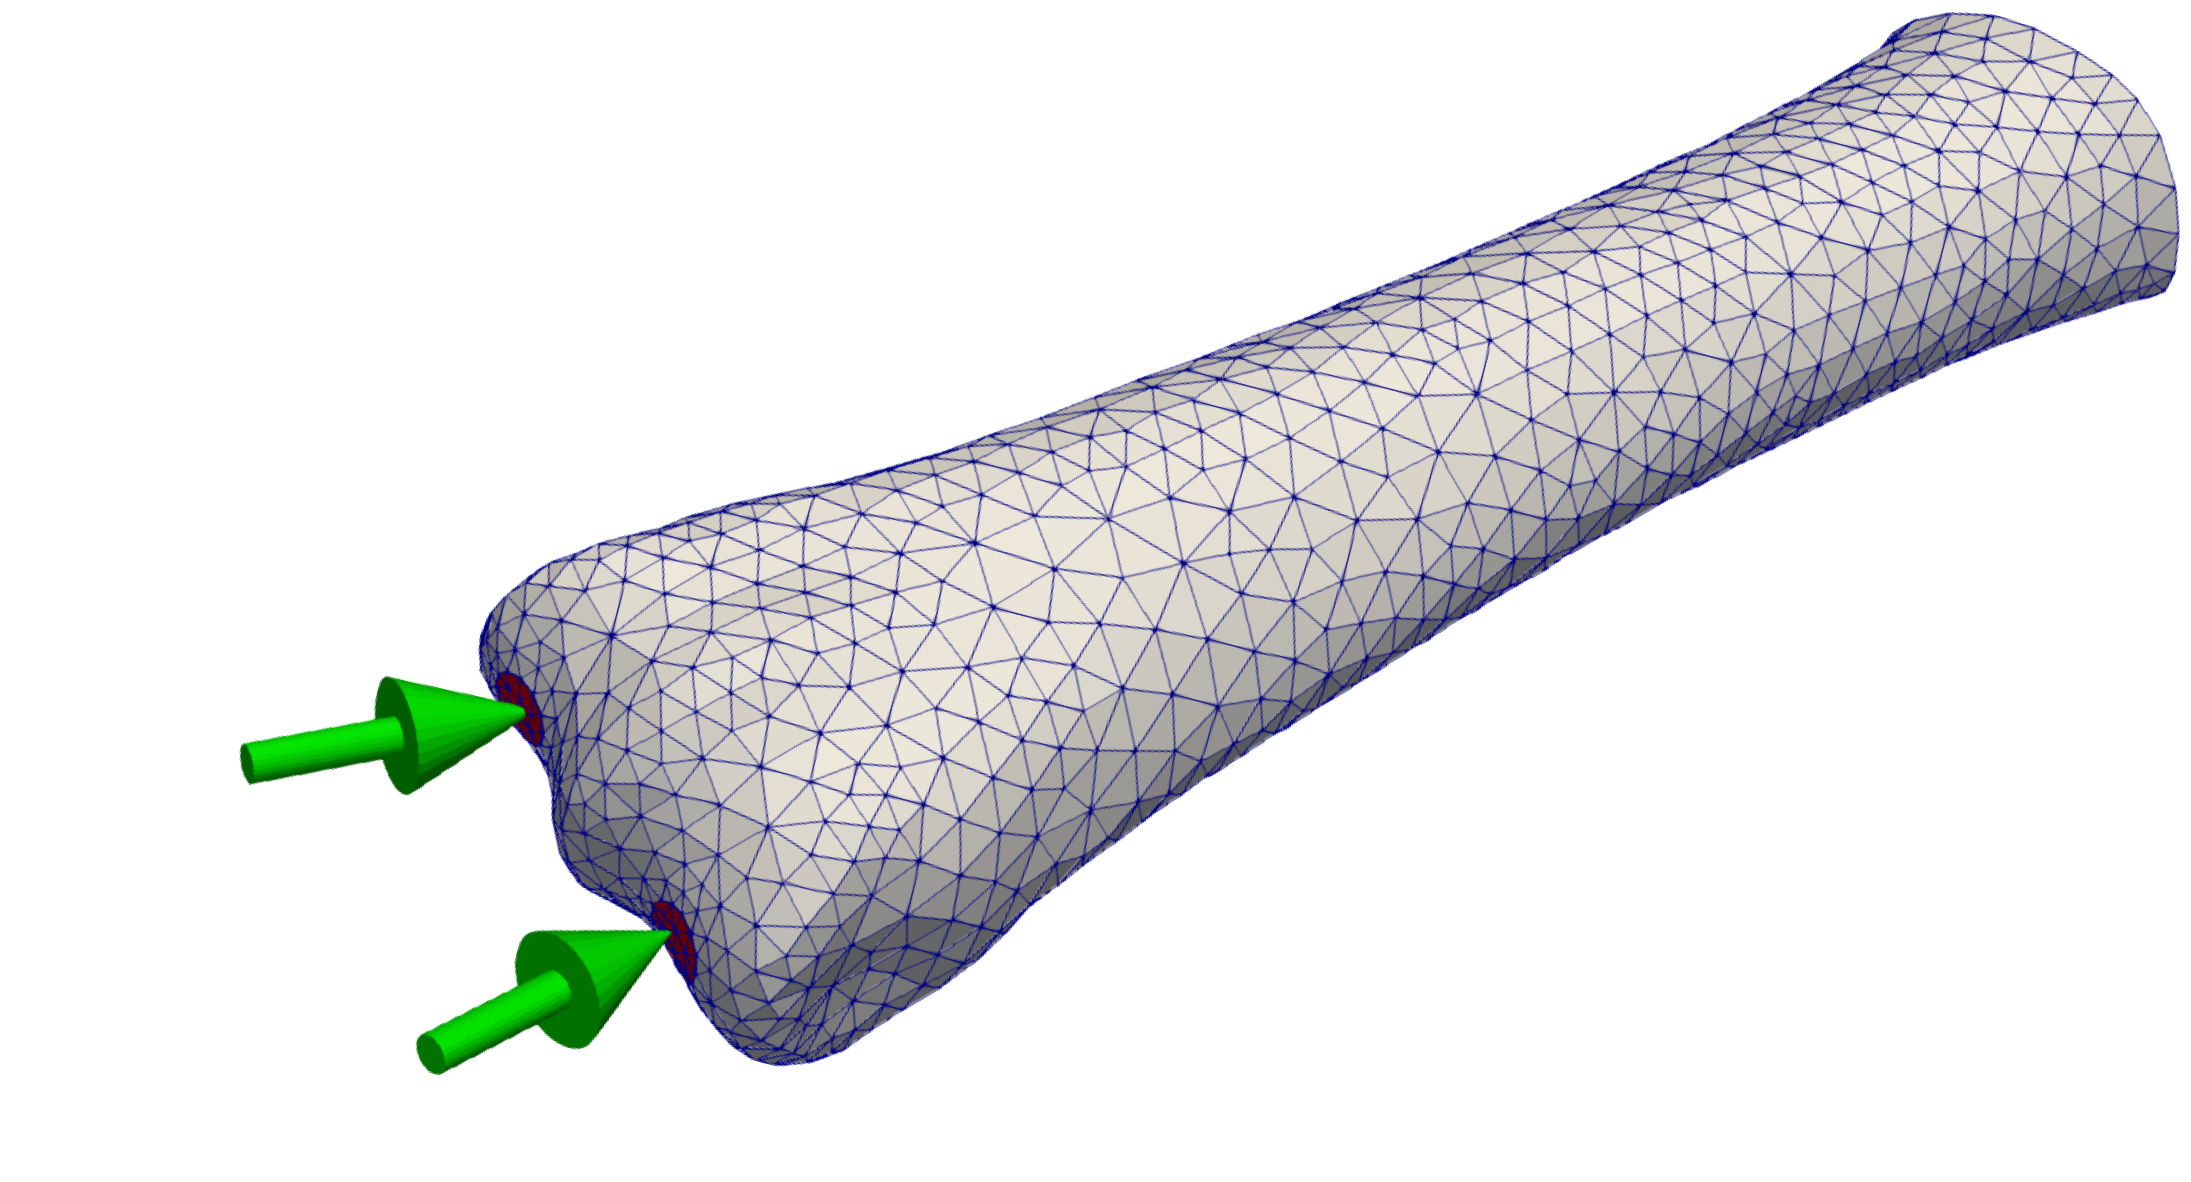
\includegraphics[width=8cm]{Figures/mc3_BC.png}};
				\node at(-3.5,-1.8){$F = 5 \mathrm{kN}$ };
				\node at(-4.1,-0.7){ $F = 5 \mathrm{kN}$ };
	\end{tikzpicture}
		\caption{Finite element mesh of the equine 3rd metacarpal bone. The subject specific three-dimensional mesh consists of 14,041 quadratic tetrahedral elements and 70,901 degrees of freedom. To simulate the peak load of a gallop, 5 kN forces are applied on the lateral and medial side of the distal condyle.}
		\label{fig:mc3_BC}
	\end{center}
\end{figure}

Results of Case~1 are presented in Figure~\ref{fig:mc3_density} where density maps at five different points in time $(\text{0, 10, 40, 100, 700})$~$[\text d]$ are visualised. 
Significant densification occurred immediately after reaching the maximum level of the loading, particularly in the proximity of the applied forces, associated with high levels of strain energy. Conversely, areas with low levels of strain energy experience a reduction in density.
After 100~$[{\text d}]$, biological equilibrium was achieved and no further changes in density took place. 
The resulting maximum density is 2.8~$[{\text {g/cm}}^3]$ and the minimum is close to zero.
\begin{figure}[h!]
	\centering
	\begin{tikzpicture}
	\node at (0,0) {	% This file was created by matlab2tikz.
%
%The latest updates can be retrieved from
%  http://www.mathworks.com/matlabcentral/fileexchange/22022-matlab2tikz-matlab2tikz
%where you can also make suggestions and rate matlab2tikz.
%
\begin{tikzpicture}

\begin{axis}[%
width=12cm,
height=8cm,
at={(0cm,0cm)},
scale only axis,
unbounded coords=jump,
xmin=0,
xmax=500,
xlabel style={font=\color{white!15!black}},
xlabel={Time [d]},
ymin=160,
ymax=270,
ylabel style={font=\color{white!15!black}},
ylabel={Mass [g]},
axis background/.style={fill=white},
legend style={legend cell align=left, align=left, draw=white!15!black}
]
\addplot [color=blue, line width=2.0pt]
  table[row sep=crcr]{%
0	248.94\\
0.5	247\\
0.638318	246.78\\
0.868834	247.79\\
1.03896	249.15\\
1.08886	249.51\\
1.17493	250.02\\
1.42765	251\\
1.73721	251.69\\
2.19611	252.06\\
2.82297	251.88\\
3.71794	250.83\\
4.99308	248.46\\
6.84533	244.13\\
9.57332	236.97\\
13.679	226.04\\
20.0215	211.27\\
29.9597	195.67\\
33.3593	191.4\\
36.7589	188.05\\
40.1584	185.43\\
41.0083	184.82\\
41.8582	184.26\\
42.7081	183.73\\
43.558	183.24\\
44.4079	182.78\\
45.2578	182.35\\
53.7568	179.51\\
71.0769	176.42\\
102.623	174.02\\
152.623	172.66\\
202.623	172.13\\
252.623	171.92\\
302.623	171.82\\
352.623	171.78\\
402.623	171.76\\
452.623	171.75\\
502.623	171.74\\
552.623	171.74\\
602.623	171.74\\
652.623	171.74\\
702.623	171.74\\
752.623	171.74\\
802.623	171.74\\
};


\addplot [color=blue, line width=2.0pt, draw=none, mark size=2.7pt, mark=triangle, mark options={solid, blue}]
  table[row sep=crcr]{%
0	248.94\\
0.5	247\\
0.638318	246.78\\
0.868834	247.79\\
1.03896	249.15\\
1.08886	249.51\\
1.17493	250.02\\
1.42765	251\\
1.73721	251.69\\
2.19611	252.06\\
2.82297	251.88\\
3.71794	250.83\\
4.99308	248.46\\
6.84533	244.13\\
9.57332	236.97\\
13.679	226.04\\
20.0215	211.27\\
29.9597	195.67\\
33.3593	191.4\\
36.7589	188.05\\
40.1584	185.43\\
41.0083	184.82\\
41.8582	184.26\\
42.7081	183.73\\
43.558	183.24\\
44.4079	182.78\\
45.2578	182.35\\
53.7568	179.51\\
71.0769	176.42\\
102.623	174.02\\
152.623	172.66\\
202.623	172.13\\
252.623	171.92\\
302.623	171.82\\
352.623	171.78\\
402.623	171.76\\
452.623	171.75\\
502.623	171.74\\
552.623	171.74\\
602.623	171.74\\
652.623	171.74\\
702.623	171.74\\
752.623	171.74\\
802.623	171.74\\
};


%\addplot [color=blue, line width=2.0pt, mark size=2.7pt, mark=triangle, mark options={solid, blue}]
 % table[row sep=crcr]{%
%nan	nan\\
%};


\end{axis}

\end{tikzpicture}% };
	\node at(0.,1.5){ 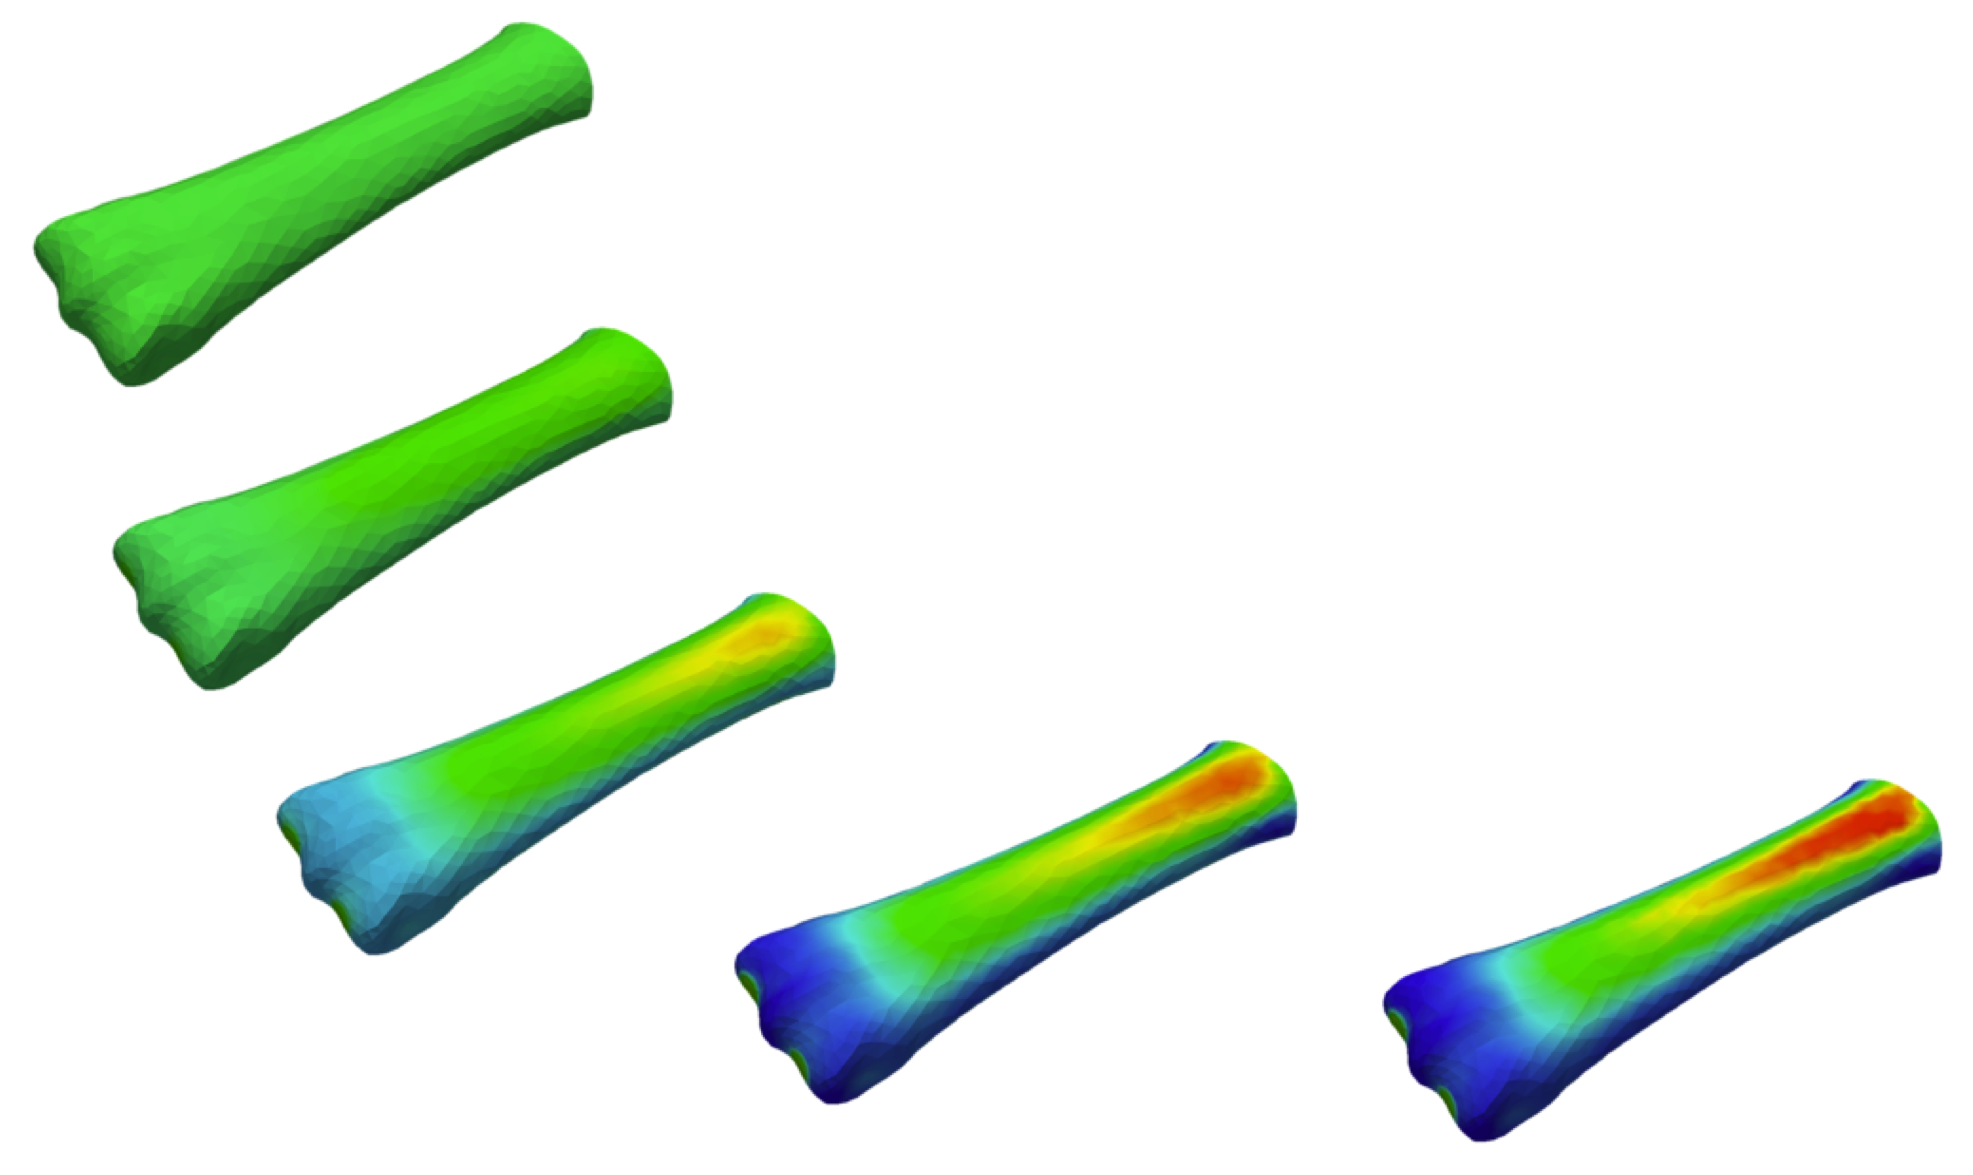
\includegraphics[width=9cm]{Figures/tikz/mc3_density_fig.png}};
	\node at(3,3){                    	\def\svgwidth{5cm} 	\input{Figures/scale_bars/scale_bar_density_rainbow.pdf_tex}  } ;
	
	\end{tikzpicture}
	%	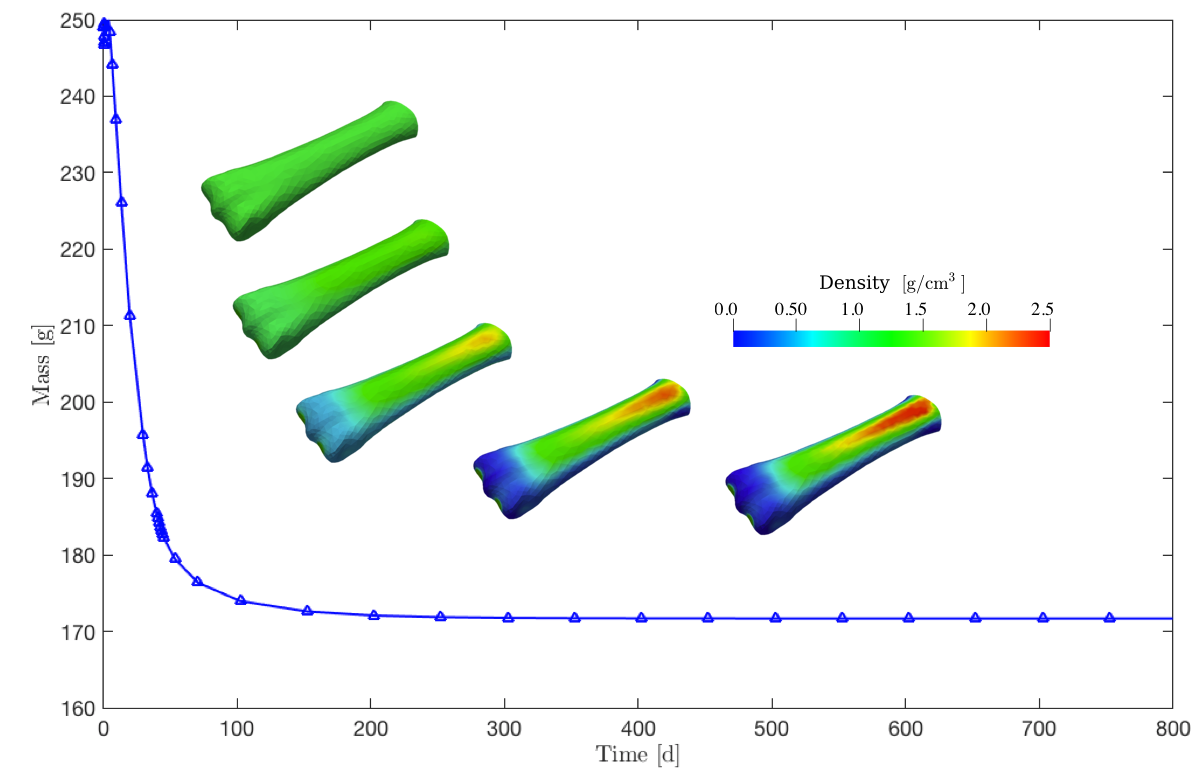
\includegraphics[width=15cm]{Figures/graphs/mc3_density.png}
	\caption{Change in overall mass of the bone over time with density evolution contours in the 3rd metacarpal at five different time points.}
	\label{fig:mc3_density}
\end{figure}



When adaptation converges to an equilibrium state, an interesting phenomenon is observed.
For each density level there is a corresponding value of constant strain energy density $\psi$
This result is a direct consequence of the constitutive Eq.~(\ref{eq:mass_source}).
This feature can be visualised by plotting the strain energy density on the contours of constant density levels as presented in Figure~\ref{fig:mc3_biol_eq}. 


\begin{figure}
	\centering
%	\begin{tikzpicture}
%	\node at (2,0) {	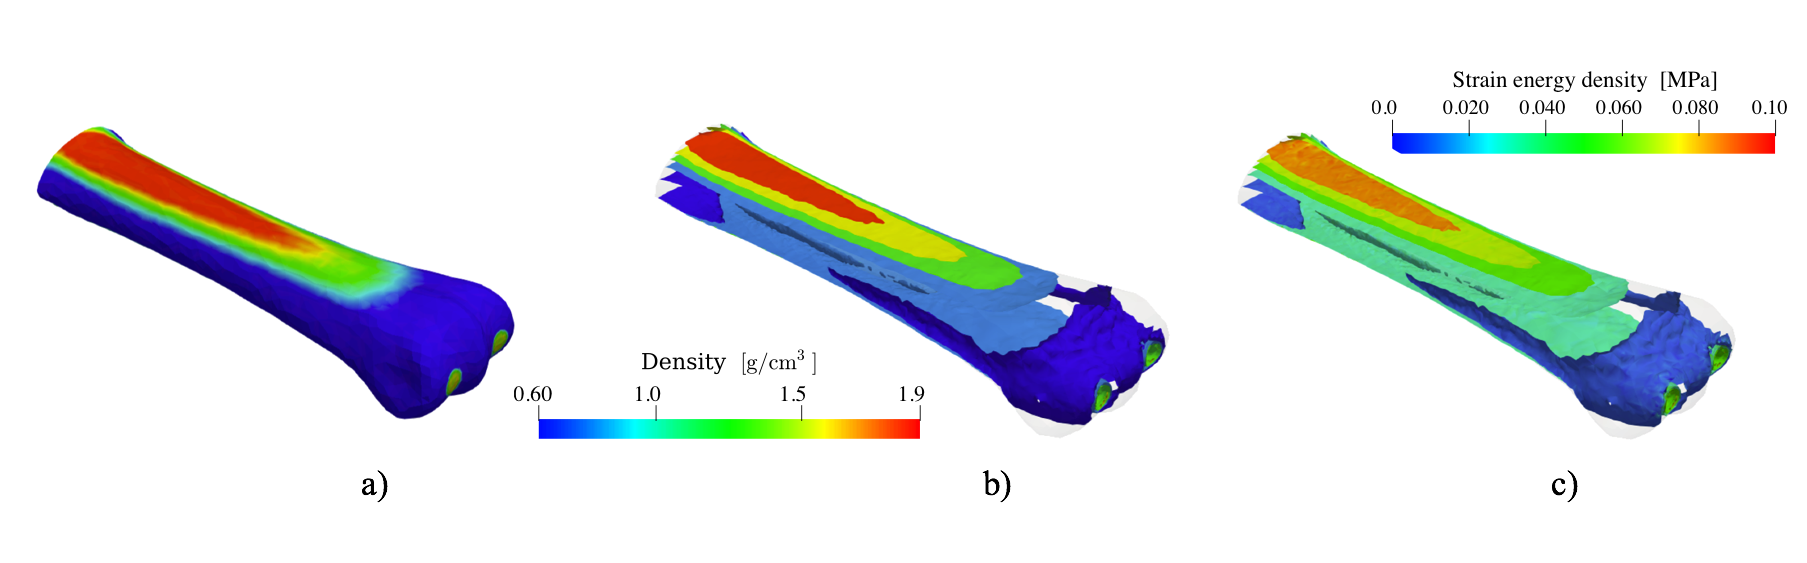
\includegraphics[width=16cm]{Figures/mc3_biol_eq.png} };
%	\node at (0.4,-0.6) {\includegraphics[width=3cm]{Figures/scale_bars/mc3_biol_eq_scale1.pdf}};
%	\node at (9,2)  {\includegraphics[width=4.5cm]{Figures/scale_bars/mc3_biol_eq_scale2.pdf}};
%	\node at (1,-2)  { a) \hspace{5cm} b) \hspace{5cm} c) };
	\def\svgwidth{14cm}
	\input{Figures/mc3_biol_eq.pdf_tex}
%	\end{tikzpicture}
	\caption{Case 1: Biological equilibrium state. a) Density map. b) Contours of density. c) Strain energy plotted on contours of density.}
	\label{fig:mc3_biol_eq}
\end{figure}


The maximum density for Case~1 is noticeably higher than in the actual equine bones~\citep{yamada2015experimental} and the minimum density is unrealistically close to zero. 
There is clearly a need to somewhat constrain upper and lower bounds for density in order to produce more realistic outcomes.
To achieve this, the bell shape function presented in Eq.~(\ref{eq:bell_function}) is used for the next two analyses (Case~2 and Case~3). 
%Therefore, in the following section, the results of two analyses with the application of the bell function (see Eq.~\ref{eq:bell_function}) are presented. 
%In the first one, the parameters for the function are: $b = 1000$, $\rho_\mathrm{max} = 2.5$~$[{\text{g/cm}}^3]$, $\rho_\mathrm{min} = 0.3$~$[{\text{g/cm}}^3]$. 
%All the rest of parameters remain unchanged. 

\begin{figure}[h!]
\centering
	%	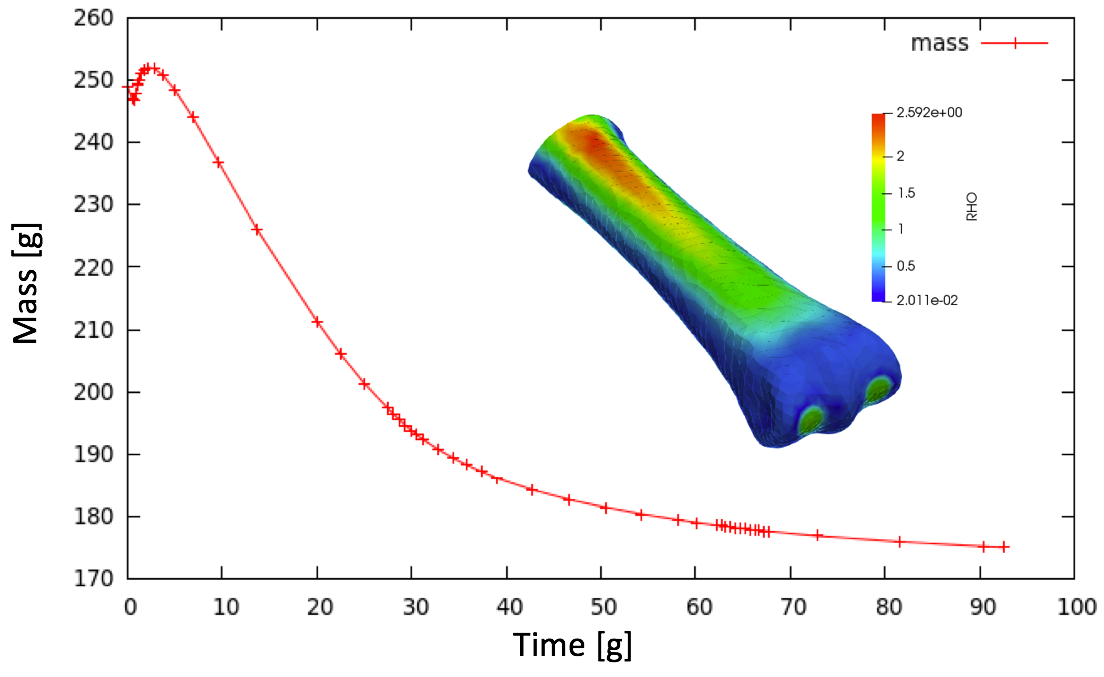
\includegraphics[width=10cm]{Figures/graphs/density_bell1.png}
			\begin{tikzpicture}
		\node at (0,0) {	% This file was created by matlab2tikz.
%
%The latest updates can be retrieved from
%  http://www.mathworks.com/matlabcentral/fileexchange/22022-matlab2tikz-matlab2tikz
%where you can also make suggestions and rate matlab2tikz.
%
\begin{tikzpicture}

\begin{axis}[%
width=6cm,
height=4cm,
at={(1.011in,0.723in)},
scale only axis,
unbounded coords=jump,
xmin=0,
xmax=100,
xlabel style={font=\color{white!15!black}},
xlabel={Time [d]},
ymin=160,
ymax=270,
ylabel style={font=\color{white!15!black}},
ylabel={Mass [g]},
axis background/.style={fill=white},
legend style={legend cell align=left, align=left, draw=white!15!black}
]
\addplot [color=blue, line width=2.0pt]
  table[row sep=crcr]{%
0	248.94\\
0.5	247\\
0.638318	246.78\\
0.868834	247.79\\
1.03896	249.15\\
1.08886	249.51\\
1.17493	250.02\\
1.42765	251\\
1.73721	251.69\\
2.19611	252.06\\
2.82297	251.88\\
3.71794	250.83\\
4.99308	248.46\\
6.84533	244.13\\
9.57332	236.97\\
13.679	226.04\\
20.0215	211.27\\
22.5061	206.03\\
24.9906	201.4\\
27.4751	197.39\\
28.0963	196.44\\
28.7174	195.53\\
29.3385	194.67\\
29.9597	193.86\\
30.5808	193.1\\
31.2019	192.38\\
32.7548	190.81\\
34.3076	189.44\\
35.8604	188.23\\
37.4133	187.16\\
38.9661	186.2\\
42.8034	184.31\\
46.6407	182.77\\
50.4781	181.48\\
54.3154	180.39\\
58.1527	179.47\\
60.1746	179.02\\
62.1966	178.61\\
62.7021	178.51\\
63.2075	178.41\\
63.713	178.31\\
64.2185	178.22\\
64.724	178.12\\
65.2295	178.03\\
65.735	177.94\\
66.2405	177.86\\
66.7459	177.77\\
67.2514	177.69\\
67.7569	177.61\\
72.8118	176.9\\
81.5878	175.97\\
90.3637	175.23\\
92.5577	175.06\\
};

\addplot [color=blue, line width=2.0pt, draw=none, mark size=1.0pt, mark=triangle, mark options={solid, blue}]
  table[row sep=crcr]{%
0	248.94\\
0.5	247\\
0.638318	246.78\\
0.868834	247.79\\
1.03896	249.15\\
1.08886	249.51\\
1.17493	250.02\\
1.42765	251\\
1.73721	251.69\\
2.19611	252.06\\
2.82297	251.88\\
3.71794	250.83\\
4.99308	248.46\\
6.84533	244.13\\
9.57332	236.97\\
13.679	226.04\\
20.0215	211.27\\
22.5061	206.03\\
24.9906	201.4\\
27.4751	197.39\\
28.0963	196.44\\
28.7174	195.53\\
29.3385	194.67\\
29.9597	193.86\\
30.5808	193.1\\
31.2019	192.38\\
32.7548	190.81\\
34.3076	189.44\\
35.8604	188.23\\
37.4133	187.16\\
38.9661	186.2\\
42.8034	184.31\\
46.6407	182.77\\
50.4781	181.48\\
54.3154	180.39\\
58.1527	179.47\\
60.1746	179.02\\
62.1966	178.61\\
62.7021	178.51\\
63.2075	178.41\\
63.713	178.31\\
64.2185	178.22\\
64.724	178.12\\
65.2295	178.03\\
65.735	177.94\\
66.2405	177.86\\
66.7459	177.77\\
67.2514	177.69\\
67.7569	177.61\\
72.8118	176.9\\
81.5878	175.97\\
90.3637	175.23\\
92.5577	175.06\\
};

\addplot [color=blue, line width=2.0pt, mark size=1.0pt, mark=triangle, mark options={solid, blue}]
  table[row sep=crcr]{%
nan	nan\\
};


\end{axis}

\end{tikzpicture}% };
		\node at(0.,1.5){ 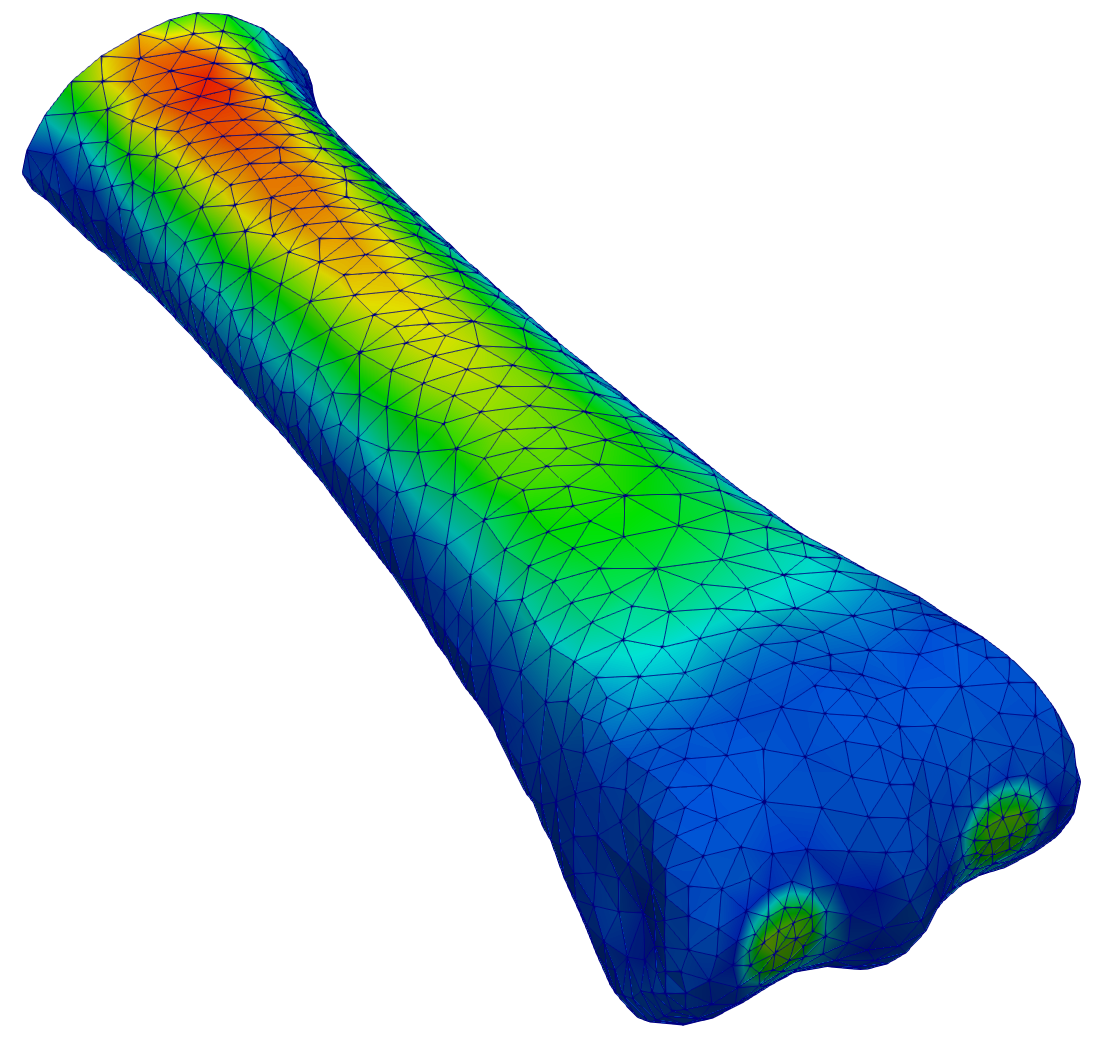
\includegraphics[width=4cm]{Figures/tikz/density_bell1_imag.png}};
		\node at(3,3){                    	\def\svgwidth{5cm} 	\input{Figures/scale_bars/scale_bar_density_rainbow.pdf_tex}  } ;
		\end{tikzpicture}
		\caption{Case~2: Change in overall mass of the bone over time with applied bell function with input parameters presented in Table~\ref{tab:three_cases}. Density distribution contours in 3rd metacarpal bone at the last converged step.}
		\label{fig:density_bell1}
\end{figure}

The results for Case~2 are plotted in Figure~\ref{fig:density_bell1}.
The last converged step takes place at $t=93$~$[{\text{d}}]$. 
By setting a high value of $b$, the transition between densities is very sharp and the algorithm encounters convergence difficulties, even with adaptive time-stepping, and biological equilibrium cannot be achieved in this case. 
However, by observing the range of densities obtained, it is evident that they slowly converge to the same solution as Case~1 (Figure~\ref{fig:mc3_density}). 
\begin{figure}[h!]
\centering
	%	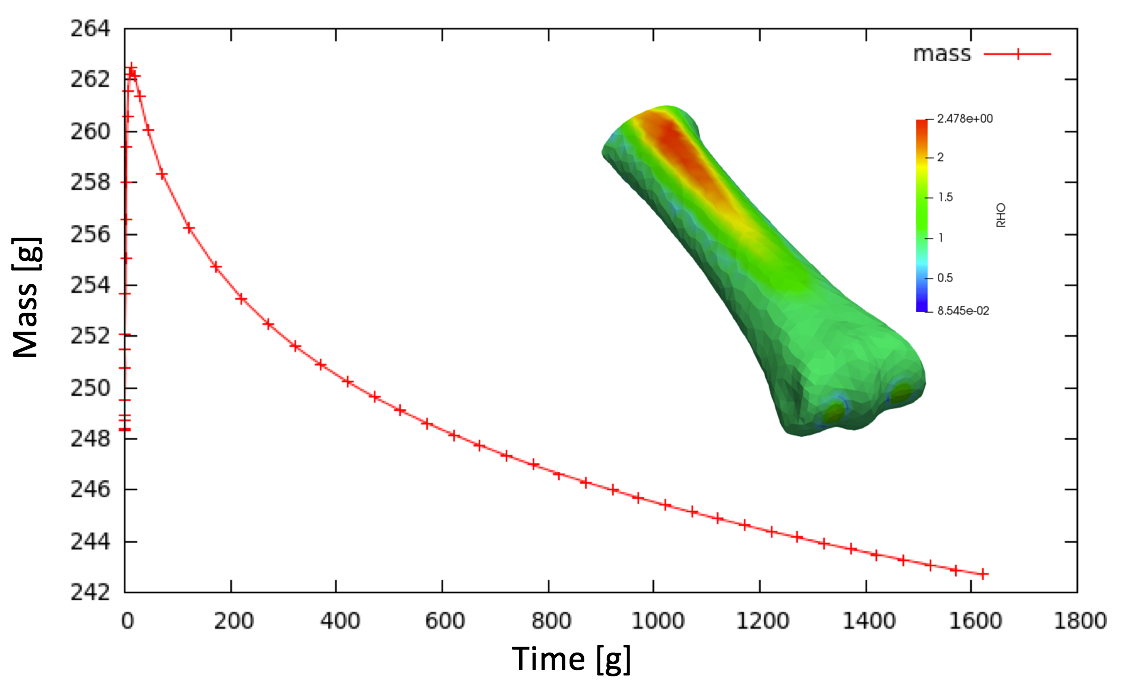
\includegraphics[width=10cm]{Figures/graphs/density_bell2.png}
				\begin{tikzpicture}
	\node at (0,0) {	% This file was created by matlab2tikz.
%
%The latest updates can be retrieved from
%  http://www.mathworks.com/matlabcentral/fileexchange/22022-matlab2tikz-matlab2tikz
%where you can also make suggestions and rate matlab2tikz.
%
\begin{tikzpicture}

\begin{axis}[%
  width=6cm,
  height=4cm,
at={(1.011in,0.723in)},
scale only axis,
unbounded coords=jump,
xmin=0,
xmax=1700,
xlabel style={font=\color{white!15!black}},
xlabel={Time [d]},
ymin=240,
ymax=270,
ylabel style={font=\color{white!15!black}},
ylabel={Mass [g]},
axis background/.style={fill=white},
legend style={legend cell align=left, align=left, draw=white!15!black}
]
\addplot [color=blue, line width=2.0pt]
  table[row sep=crcr]{%
0	248.94\\
0.5	248.36\\
0.625	248.4\\
0.75	248.75\\
0.875	249.53\\
1	250.79\\
1.0803	251.51\\
1.15271	252.1\\
1.41315	253.69\\
1.70451	255.06\\
2.1455	256.56\\
2.73899	257.99\\
3.58705	259.36\\
4.78935	260.58\\
6.53053	261.57\\
9.08236	262.23\\
12.8971	262.46\\
18.6862	262.19\\
27.8059	261.39\\
43.2273	260.08\\
71.3203	258.31\\
121.32	256.23\\
171.32	254.7\\
221.32	253.48\\
271.32	252.48\\
321.32	251.62\\
371.32	250.88\\
421.32	250.22\\
471.32	249.63\\
521.32	249.1\\
571.32	248.61\\
621.32	248.16\\
671.32	247.74\\
721.32	247.35\\
771.32	246.98\\
821.32	246.64\\
871.32	246.31\\
921.32	246\\
971.32	245.7\\
1021.32	245.41\\
1071.32	245.14\\
1121.32	244.88\\
1171.32	244.63\\
1221.32	244.38\\
1271.32	244.15\\
1321.32	243.92\\
1371.32	243.7\\
1421.32	243.49\\
1471.32	243.28\\
1521.32	243.08\\
1571.32	242.89\\
1621.32	242.7\\
};

\addplot [color=blue, line width=2.0pt, draw=none, mark size=1.0pt, mark=triangle, mark options={solid, blue}]
  table[row sep=crcr]{%
0	248.94\\
0.5	248.36\\
0.625	248.4\\
0.75	248.75\\
0.875	249.53\\
1	250.79\\
1.0803	251.51\\
1.15271	252.1\\
1.41315	253.69\\
1.70451	255.06\\
2.1455	256.56\\
2.73899	257.99\\
3.58705	259.36\\
4.78935	260.58\\
6.53053	261.57\\
9.08236	262.23\\
12.8971	262.46\\
18.6862	262.19\\
27.8059	261.39\\
43.2273	260.08\\
71.3203	258.31\\
121.32	256.23\\
171.32	254.7\\
221.32	253.48\\
271.32	252.48\\
321.32	251.62\\
371.32	250.88\\
421.32	250.22\\
471.32	249.63\\
521.32	249.1\\
571.32	248.61\\
621.32	248.16\\
671.32	247.74\\
721.32	247.35\\
771.32	246.98\\
821.32	246.64\\
871.32	246.31\\
921.32	246\\
971.32	245.7\\
1021.32	245.41\\
1071.32	245.14\\
1121.32	244.88\\
1171.32	244.63\\
1221.32	244.38\\
1271.32	244.15\\
1321.32	243.92\\
1371.32	243.7\\
1421.32	243.49\\
1471.32	243.28\\
1521.32	243.08\\
1571.32	242.89\\
1621.32	242.7\\
};


\addplot [color=blue, line width=2.0pt, mark size=1.0pt, mark=triangle, mark options={solid, blue}]
  table[row sep=crcr]{%
nan	nan\\
};

\end{axis}
\end{tikzpicture}% };
	\node at(0.,1.5){ 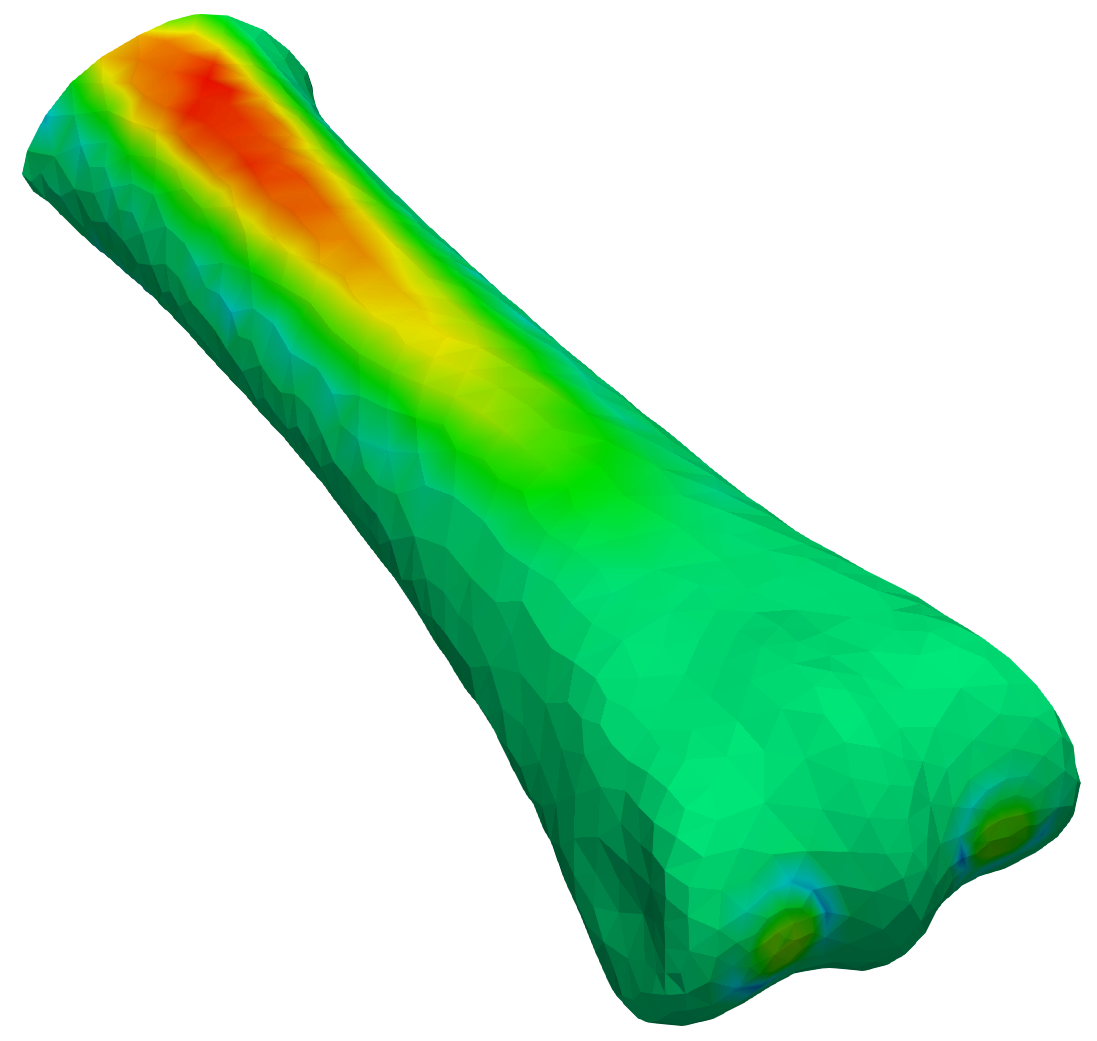
\includegraphics[width=4cm]{Figures/tikz/density_bell2_imag.png}};
	\node at(3,3){                    	\def\svgwidth{5cm} 	\input{Figures/scale_bars/scale_bar_density_rainbow.pdf_tex}  } ;
	\end{tikzpicture}
	
		\caption{Case~3: Change in overall mass of the bone over time with applied bell function with input parameters presented in Table~\ref{tab:three_cases}. Density distribution contours in 3rd metacarpal bone at time step $t=1600$~$[{\text{d}}]$.}
		\label{fig:density_bell2}
\end{figure}

For Case~3, a more moderate value for the exponent in the bell function was chosen along with a narrower density range than those chosen for Case~2 (see Table~\ref{fig:mc3_biol_eq}).
The plot presented in Figure~\ref{fig:density_bell2} demonstrates how these values influence the results of the analysis. 
It is evident that with a much lower value for exponent, $b$, the algorithm no longer has problems converging. 
Furthermore,  reducing the range between the upper and lower bounds of density have a significant impact on the results. 
The dense cortical shaft on the dorsal side of the bone is less dense and covers a much larger region. 
Furthermore, unrealistically low values of densities have been eliminated. 
However, as with the previous case, the overall solution converges to the same mass (and density distribution) as in Case~1, albeit requiring significantly more time steps. \\
%In the next sections, the methods will be presented on how to map the resulting density patterns from bone adaptation analysis on different meshes by using moving least squares approximation. Subsequently, the new model will be used to estimate the propensity to fracture, by calculating material forces on the introduced crack tip.
\subsection{MLS mapping examples}
\label{sec:mals_mapping}
Here, validation of the implementation of the MLS method (described in Section~\ref{sec:mwls}) is presented via two examples.
The first example involves the mapping of an analytical scalar field onto the nodes of a mesh of a prism.
For this case, the relative error between the analytical input scalar field and MLS results are compared for three target orders of approximation of MLS.
In the second example, mapping of CT scan data of a bone onto a mesh is presented.
For this challenging mesh geometry, results of the MLS method are compared with the direct CT scan data as well as results of least squares method.
    
\subsubsection{Mapping of analytical field}
The analytical field ($f({\boldsymbol {\rm x}})=x + y^2 + z^3 $) %(simulating CT scan data). 
is mapped onto the mesh nodes of the prism (Figure~{\ref{fig:mwlsprism}a}) using the proposed MLS procedure described in Section~\ref{sec:mwls}.
The analytical field $f({\boldsymbol {\rm x}})$ is evaluated at a discrete set of points, $v({\boldsymbol{\rm x}}_i)$, presented in Figure~\ref{fig:mwlsprism}b.
The FE mesh is placed within the discrete field (Figure~\ref{fig:mwlsprism}b) and the spherical domains of influence of each mesh node are presented (reduced in size for clearer visual presentation) in Figure~\ref{fig:mwlsprism}c. 
The size of the influence domain is determined by increasing its radius until matrix $\mathbf A$ in Eq.~(\ref{eq:mwls_system}) is invertible for all mesh nodes. 
The approximated field data, with its gradient, is saved on corresponding nodes as demonstrated in Figure~\ref{fig:mwlsprism}c for $q=10$. 
Subsequently, the relative approximation error between the norm of analytical gradient of the given field $f({\boldsymbol {\rm x}})$ at the coordinates of each mesh node and the norm of gradient calculated with MLS at the same node is evaluated and presented in Figure~\ref{fig:prism_error}.
The error is evaluated for three cases: constant ($q=1$), linear ($q=4$) and quadratic ($q=10$) basis functions. 
It is clear from presented results in Figure~\ref{fig:prism_error} that constant functions are not sufficient for evaluating the gradient. 
The maximum error for a linear and quadratic basis has values of $10^{-2}$ and $10^{-4}$, respectively. 
These results are satisfactory for the application of mapping data fields onto the mesh and suggests correctness of the implementation.
\begin{figure}[h!]
	\centering
%	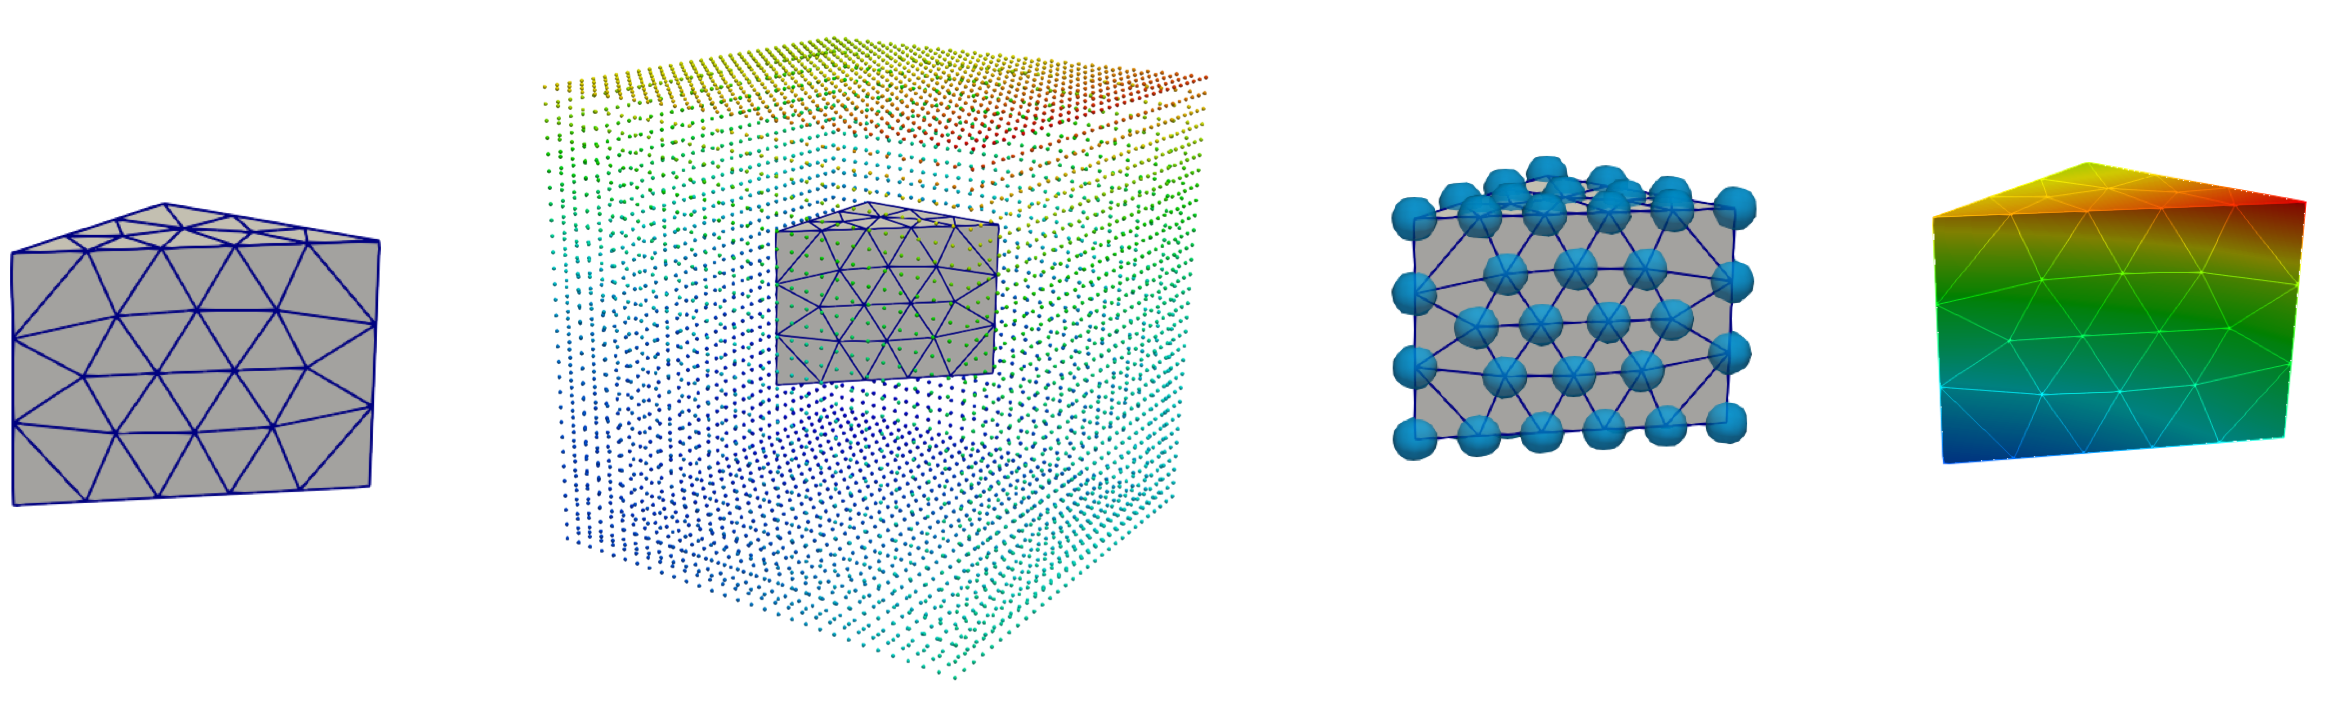
\includegraphics[width=16cm]{Figures/mwls_prism.png}
	\begin{tikzpicture}
	%	\node at (0,0) {		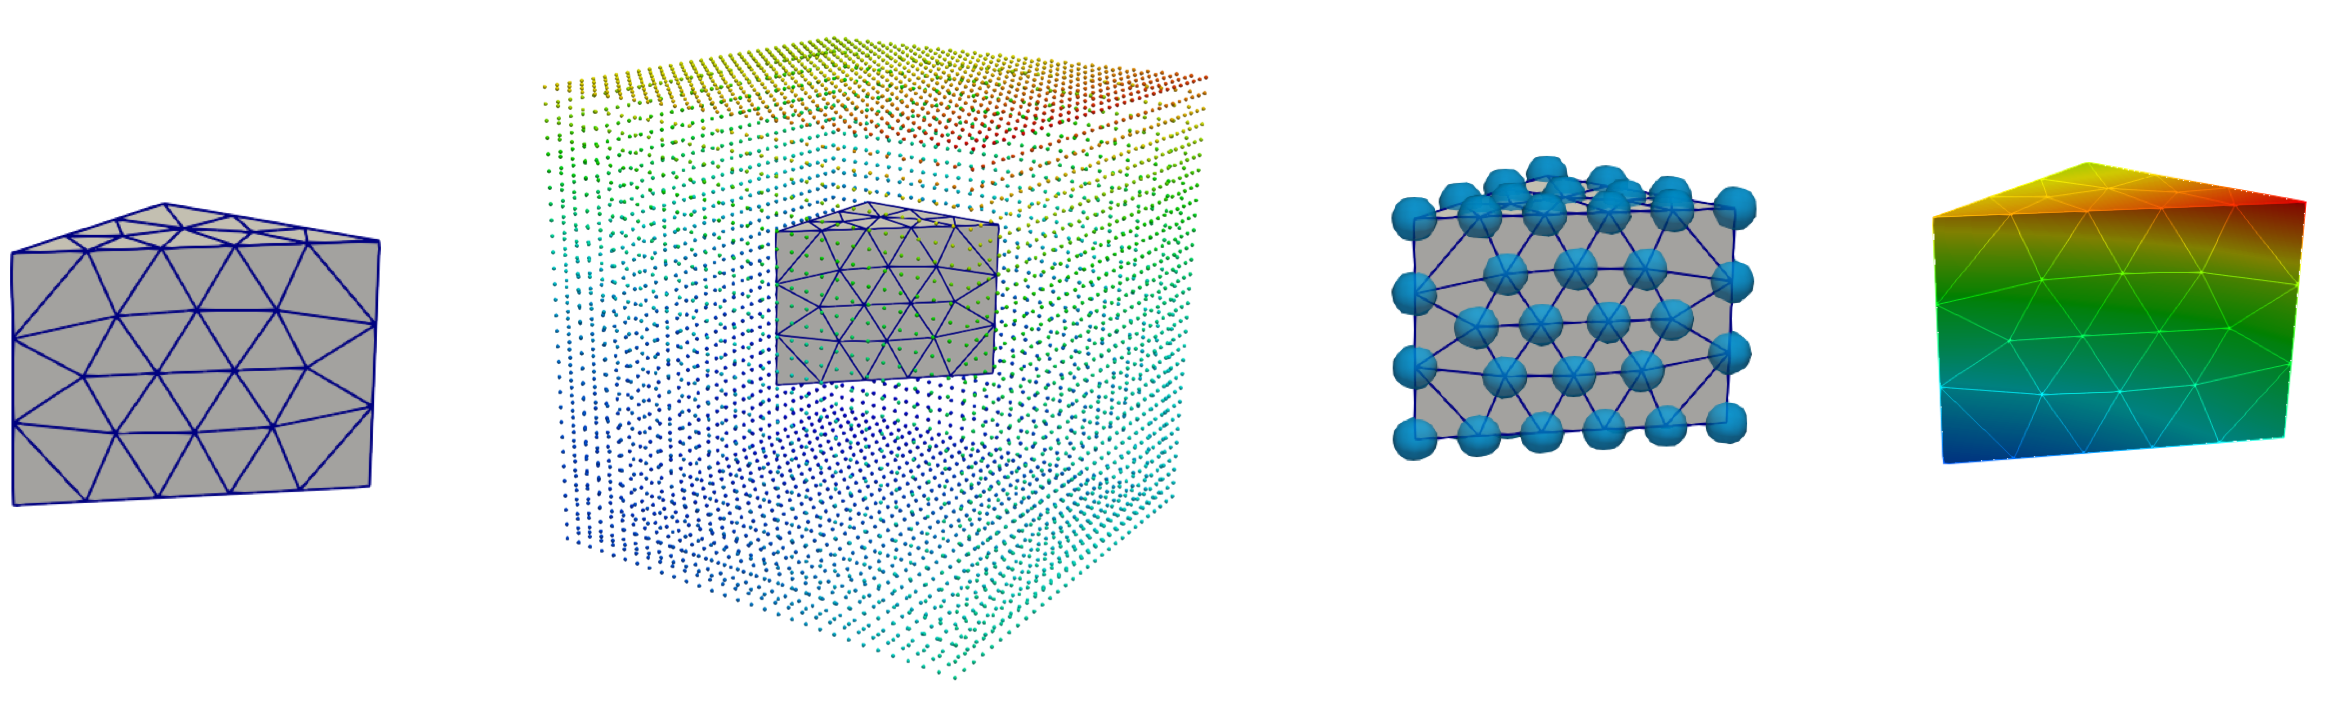
\includegraphics[width=14cm]{Figures/mwls_prism.png} };
		\node at(-1,-2){a) \hspace{3cm} b)  \hspace{4.5cm}   c)  \hspace{3cm}  d)     };
	\end{tikzpicture}
	\caption{a) Finite element tetrahedral mesh. b) Mesh inside analytical discrete field $f({\boldsymbol {\rm x}}) = x + y^2 + z^3$. c) Mesh with corresponding nodes and spherical domain of influence. d) Outcomes of the approximation for $q=10$.}
	\label{fig:mwlsprism}
\end{figure}
\begin{figure}[h!]
	\centering
	%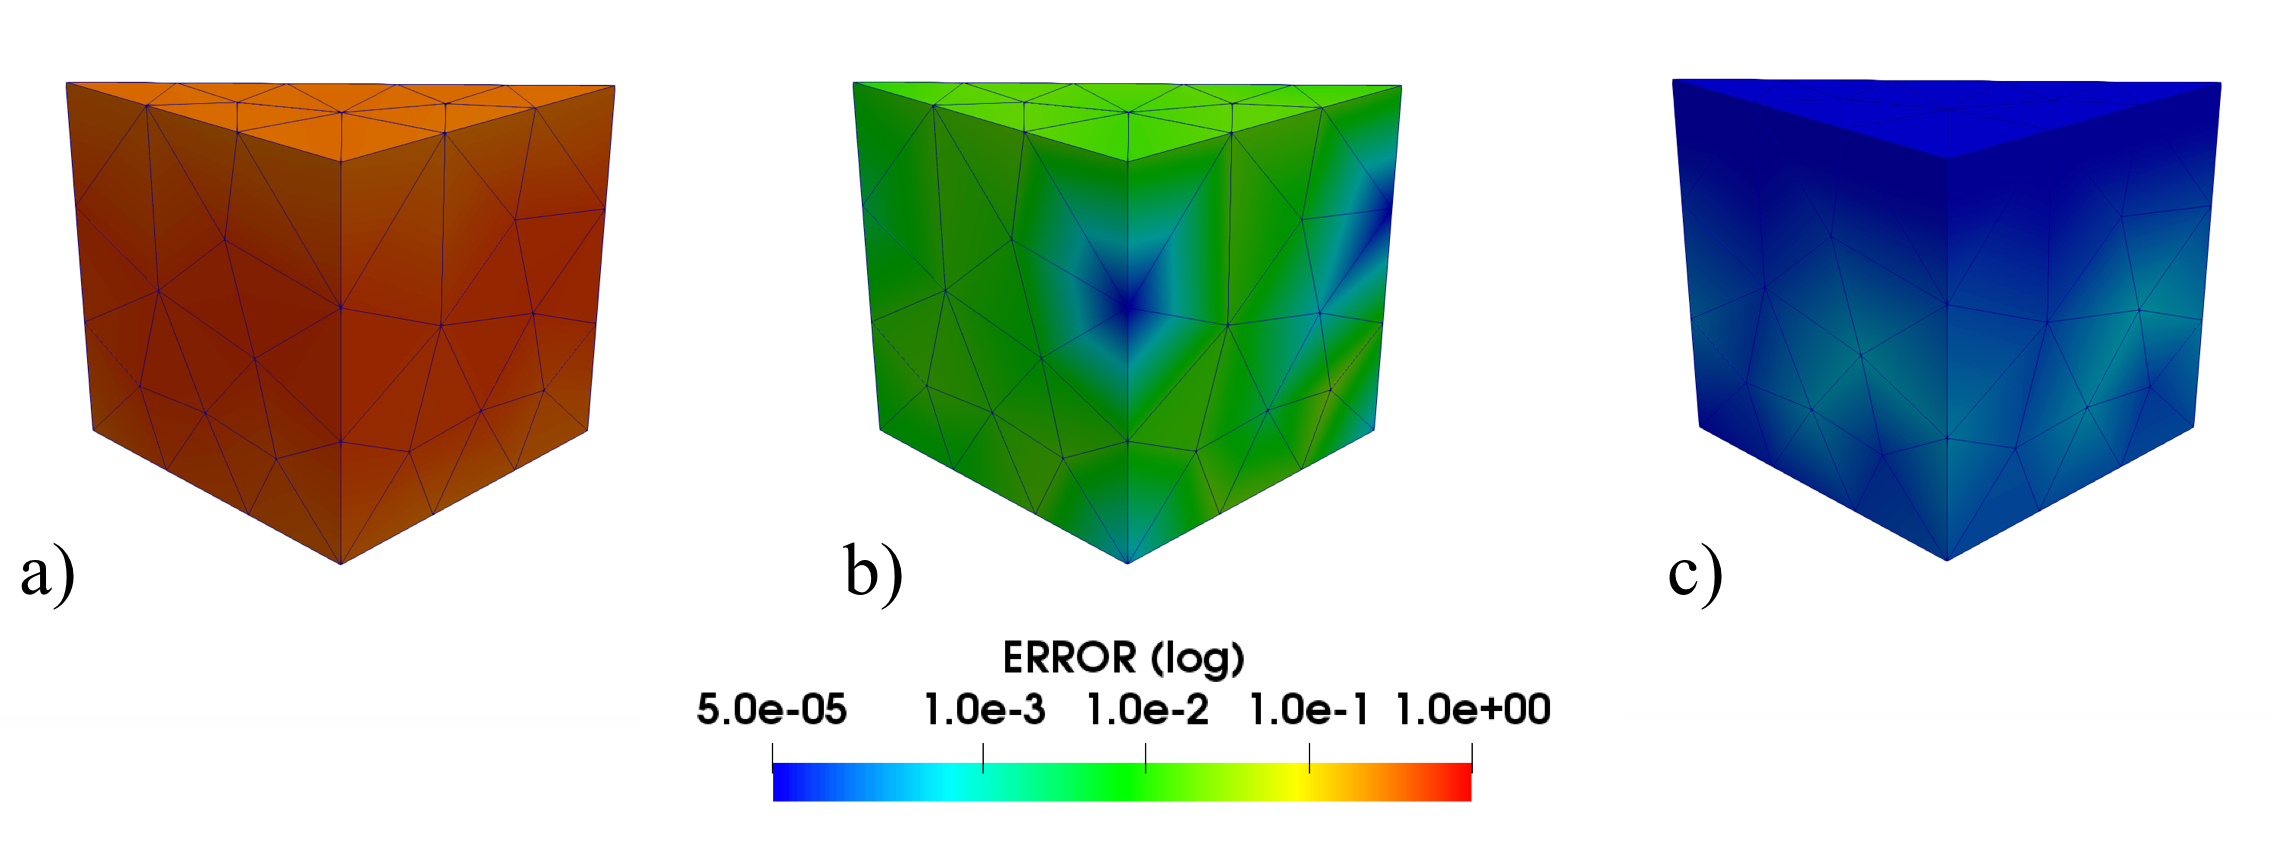
\includegraphics[width=10cm]{Figures/prism_error.png}
		\def\svgwidth{14cm}
	\input{Figures/prism_error.pdf_tex}
	\caption{Contour plot of relative error of approximated gradient field for constant a), linear b) and quadratic c) basis functions. The logarithmic scale represents the magnitude of relative error.}
	\label{fig:prism_error}
\end{figure}
\subsubsection{Metacarpal bone}
In this section, the results of density approximation from CT data are presented. Geometry and finite element mesh of an equine 3rd metacarpal bone was obtained in ScanIP (Synopsys Simpleware, Exeter) from medical 3D images. The data was subsequently used to approximate the density values onto finite element mesh nodes by using implemented MLS method. 
The mesh used is consisted of approximately 7000 tetrahedral elements.
\begin{figure}
	\centering
	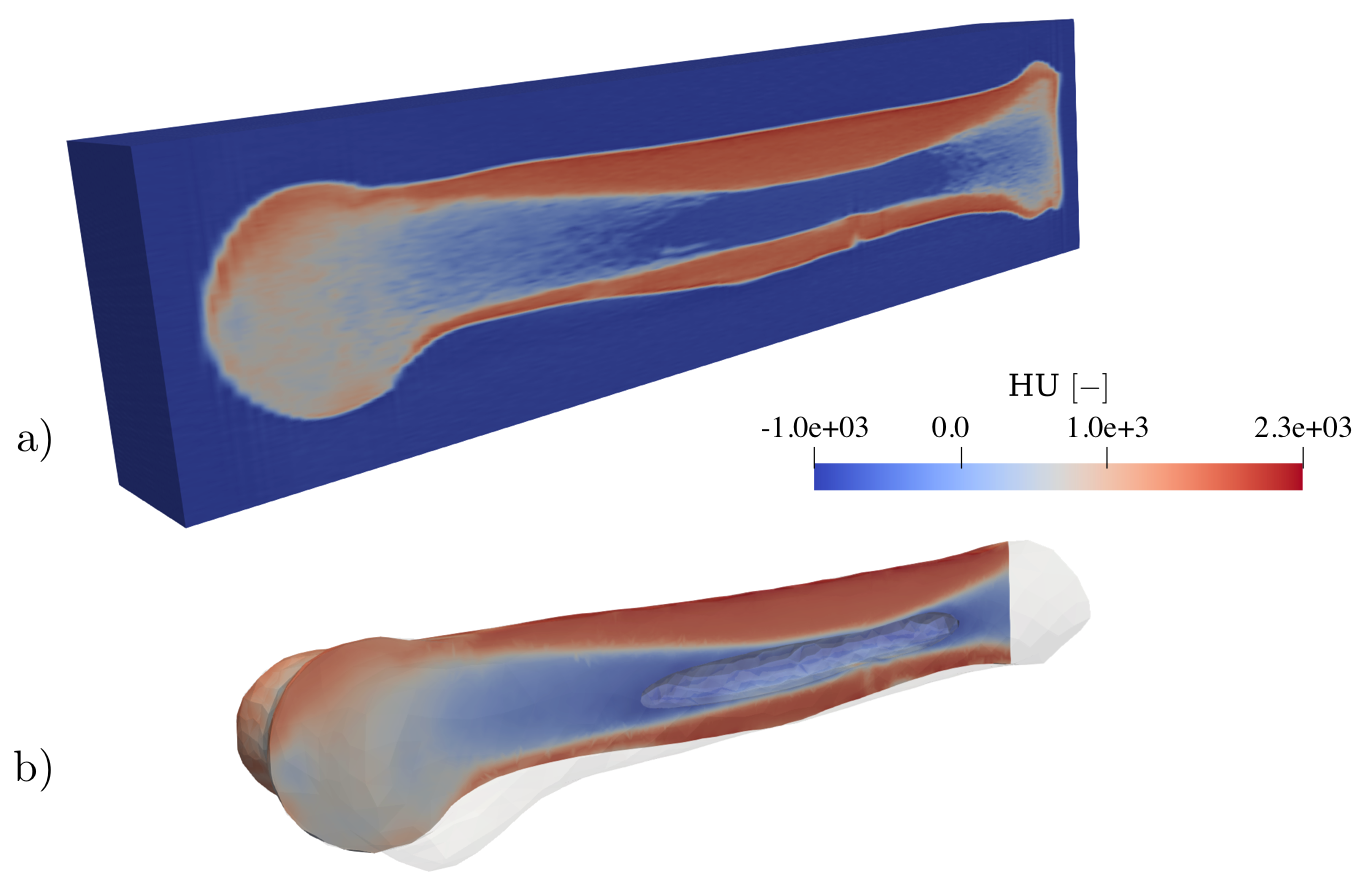
\includegraphics[width=0.5\linewidth]{Figures/mwlsmapping_cross.png}
	\caption{Comparison of a CT data with the corresponding approximation. a) A cut-view along the $x-y$ plane for CT scan data and b) density mapped onto FE mesh.}
	\label{fig:mwlsmapping_cross}
\end{figure}
Results of the mapping procedures are presented in Figure~\ref{fig:mwlsmapping_cross}. Comparison to CT data and the standard Least Squares (LS) method in classical finite element method framework are demonstrated in Figure~\ref{fig:mwlsmappingcomparisons}.
\begin{figure}
	\centering
	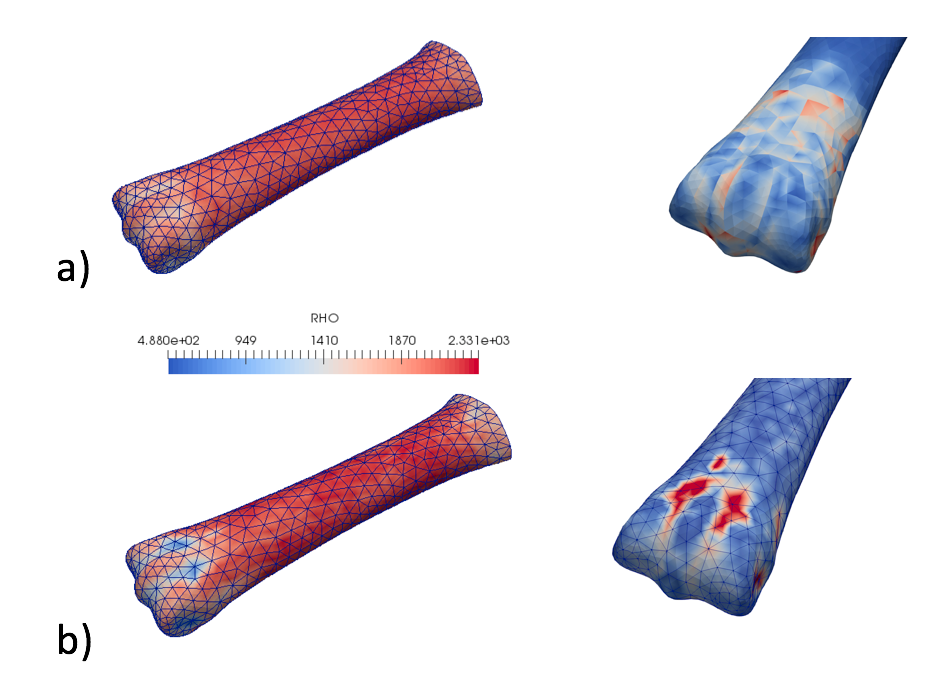
\includegraphics[width=0.7\linewidth]{Figures/mwls_mapping_comparisons.png}
	\caption{Mapping results of bone density (left) and density gradient (right). a) Least squares approximation. b)~Moving least squares approximation.}
	\label{fig:mwlsmappingcomparisons}
\end{figure}
Mapped density pattern from both methods is very similar. 
Thanks to the approximation, the obtained field is continuous despite the fact that the mesh is relatively coarse. 
It is especially beneficial in case of hierarchical basis framework where larger elements with high order approximation are more desired. 
Classic finite element method provides only ${C^0}$-continuity; therefore the results of gradients obtained with LS are only piecewise continuous. 
Gradients form MLS, on the contrary, are smooth, which can be of great importance when the mapping is used in crack propagation analysis since it strongly influences the direction of a crack. 
It can also be seen that mesh boundary does not suffer from Partial Volume Artifacts~\citep{adams2009quantitative}.
%try more meshes maybe?
\subsection{Stress intensity calculations}
\label{sec:release_energy_rate}
In this section five numerical examples of calculating material forces are presented. 
To validate the correctness of the implementation, first, a simple quasi-two-dimensional plate with homogeneous material distribution is considered. 
The convergence study is performed by comparing results to the analytical solution. 
In the next section, quarter point elements and their influence on the convergence rate are presented. 
In the third subsection, the results with the heterogeneous material are presented, along with proposed validation. 
The last two examples demonstrate the calculation of material forces for bones.  
\subsubsection{Finite plate with a horizontal crack}\label{sec:plate_section}
All input parameters presented in this study are dimensionless. 
This example involves finite plate with height, $h_{\rm {pl}} = 10$, thickness $t_{\rm {pl}}=1$ and half width $b_{\rm{pl}} = 2.5$ and a horizontal through-thickness crack with half width $a_{\rm {pl}} = 1$ as presented in Figure~\ref{fig:plate_load_mesh}a).
The finite plate is spatially discretised using 1384 tetrahedral elements and subjected to uniaxial stress along the height direction as indicated in Figure~\ref{fig:plate_load_mesh}b. 
Furthermore, displacements are constrained at three vertices of the plate to prevent rigid body motions. 
%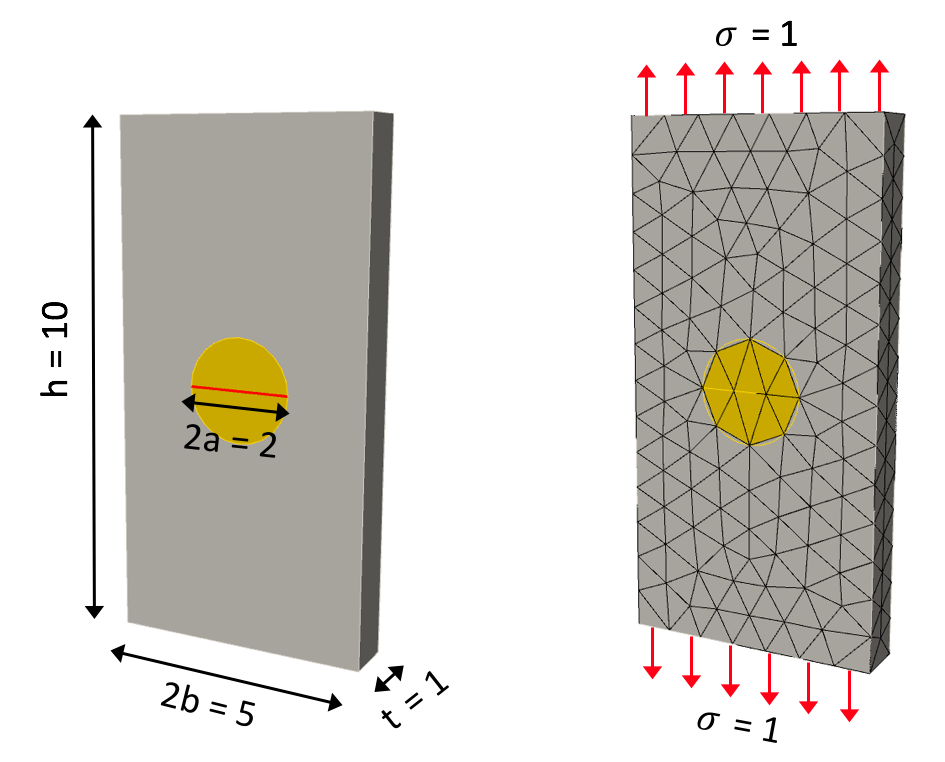
\includegraphics[width=0.5\linewidth]{Figures/plate_load_mesh.png}

\begin{figure}[h!]
\begin{center}
\begin{tabular}{c c c c}
 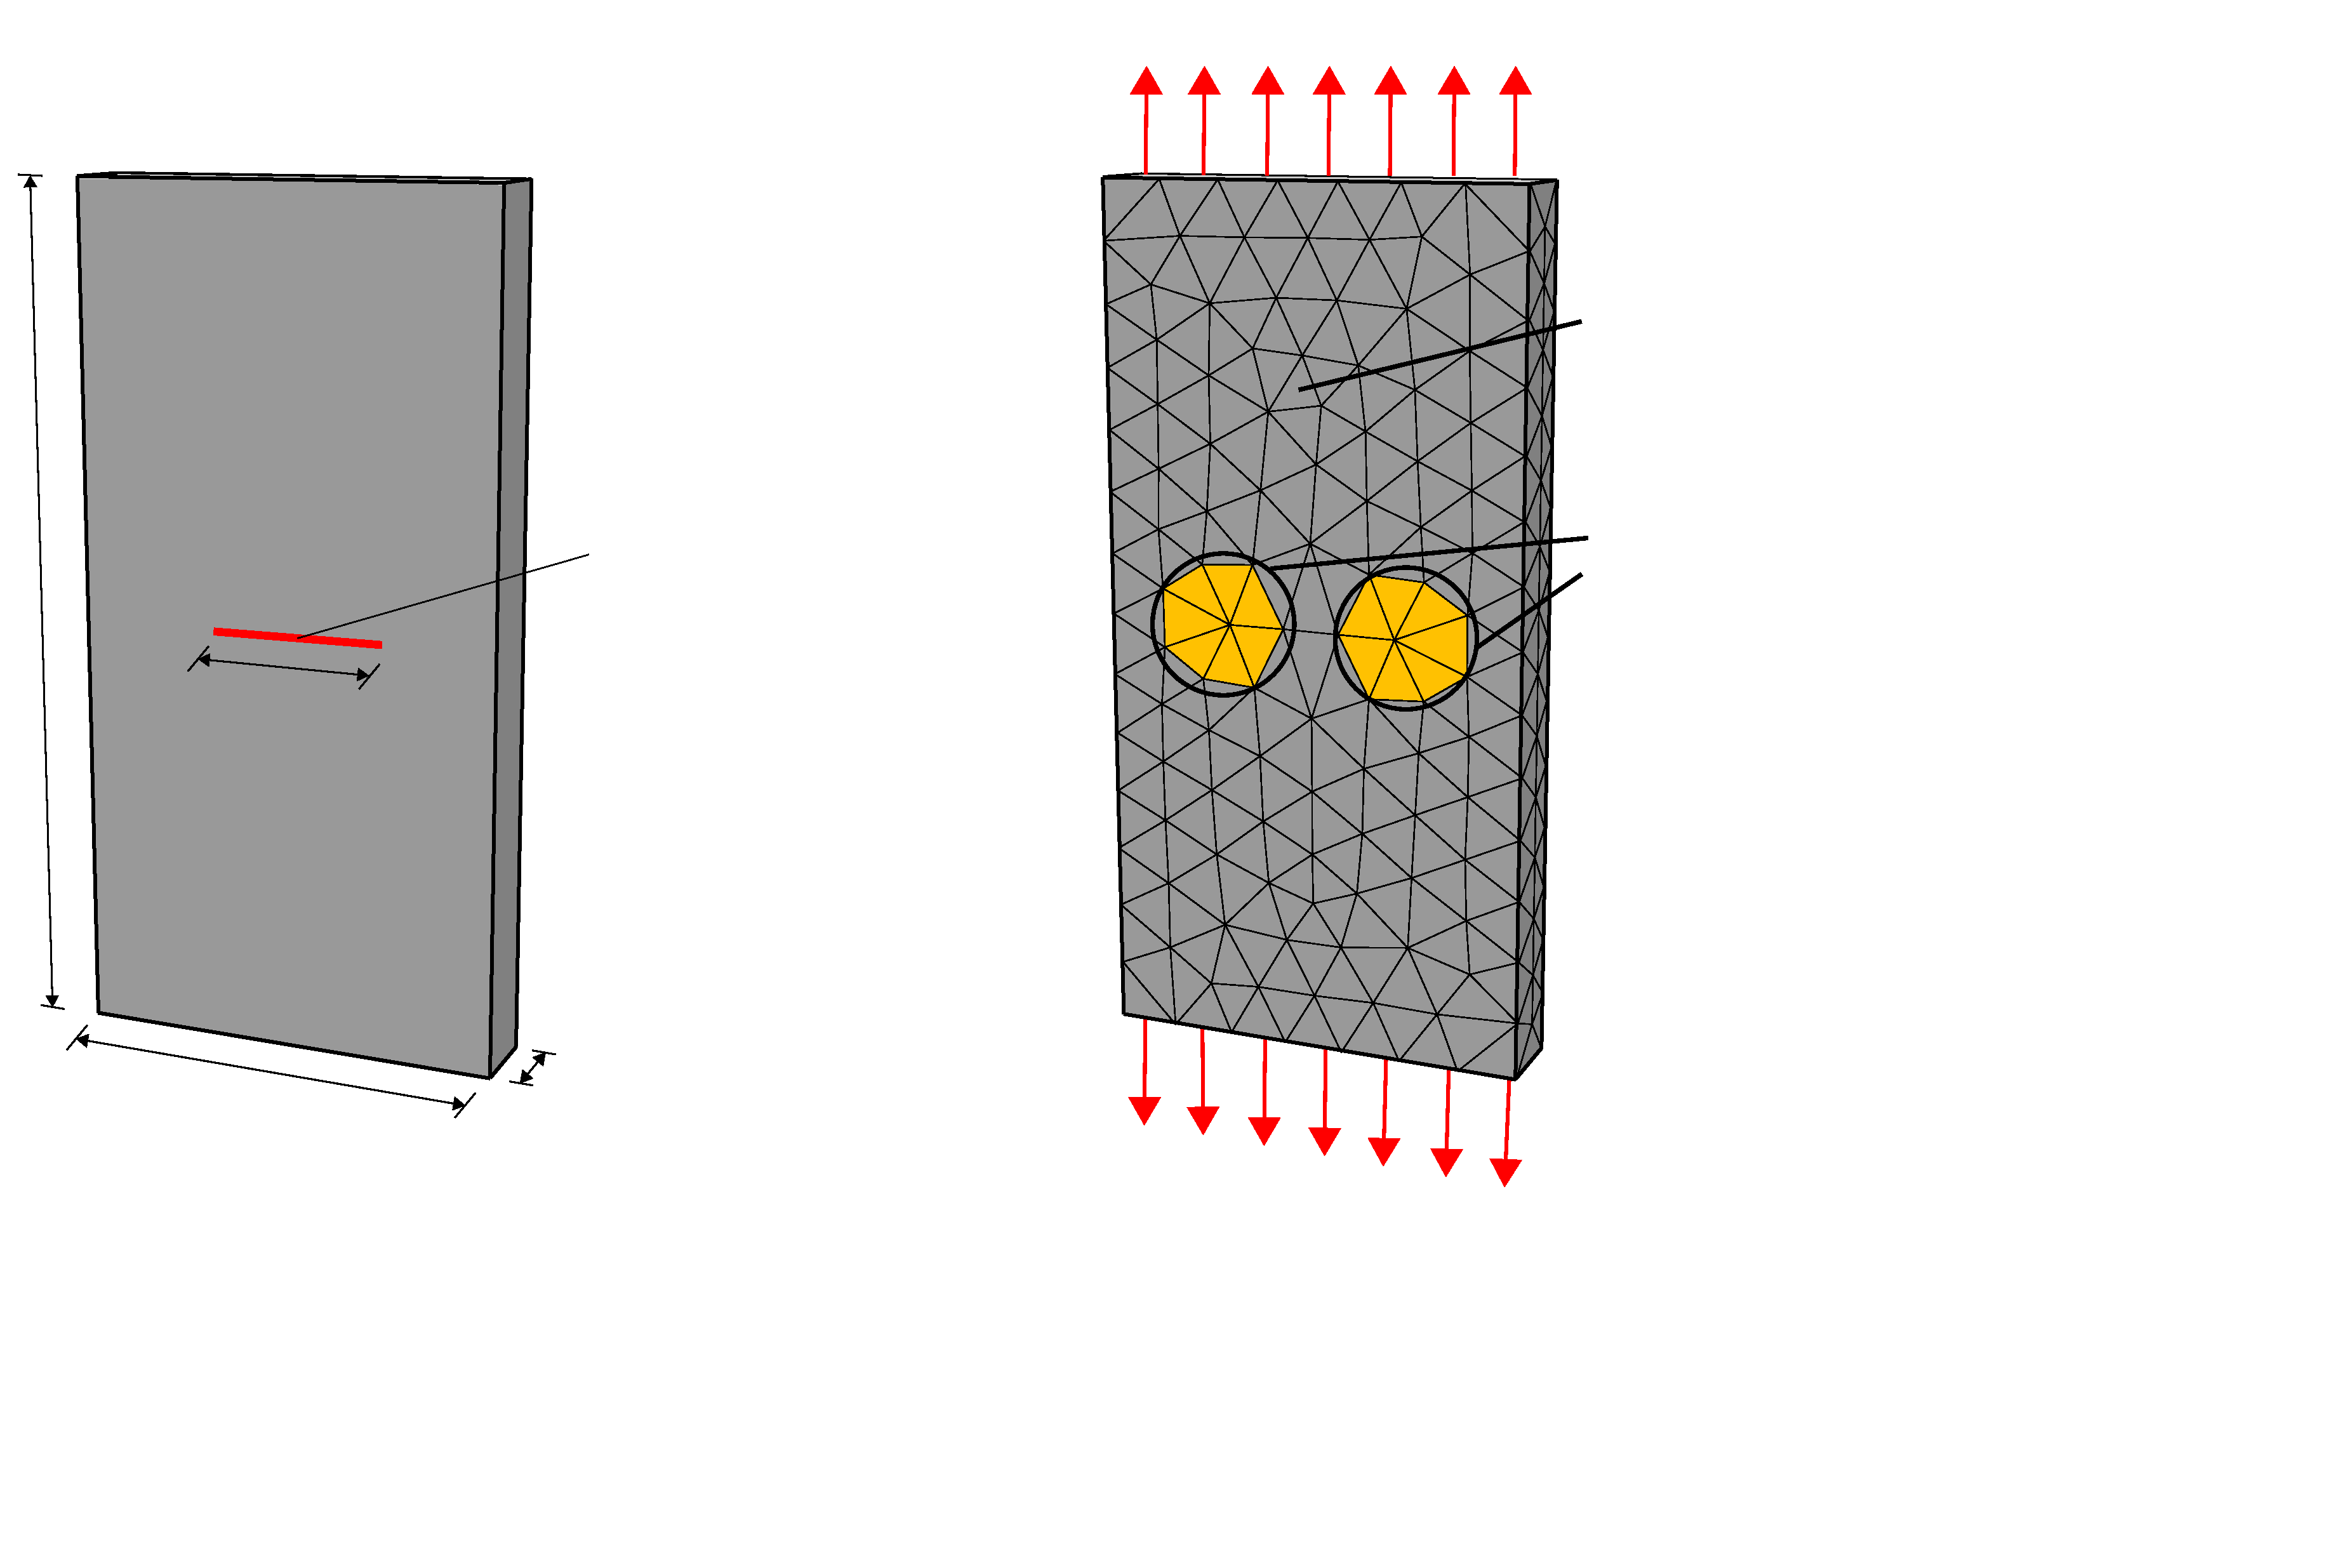
\includegraphics[height=8.5cm]{Figures/InfSlab.pdf} & &   & {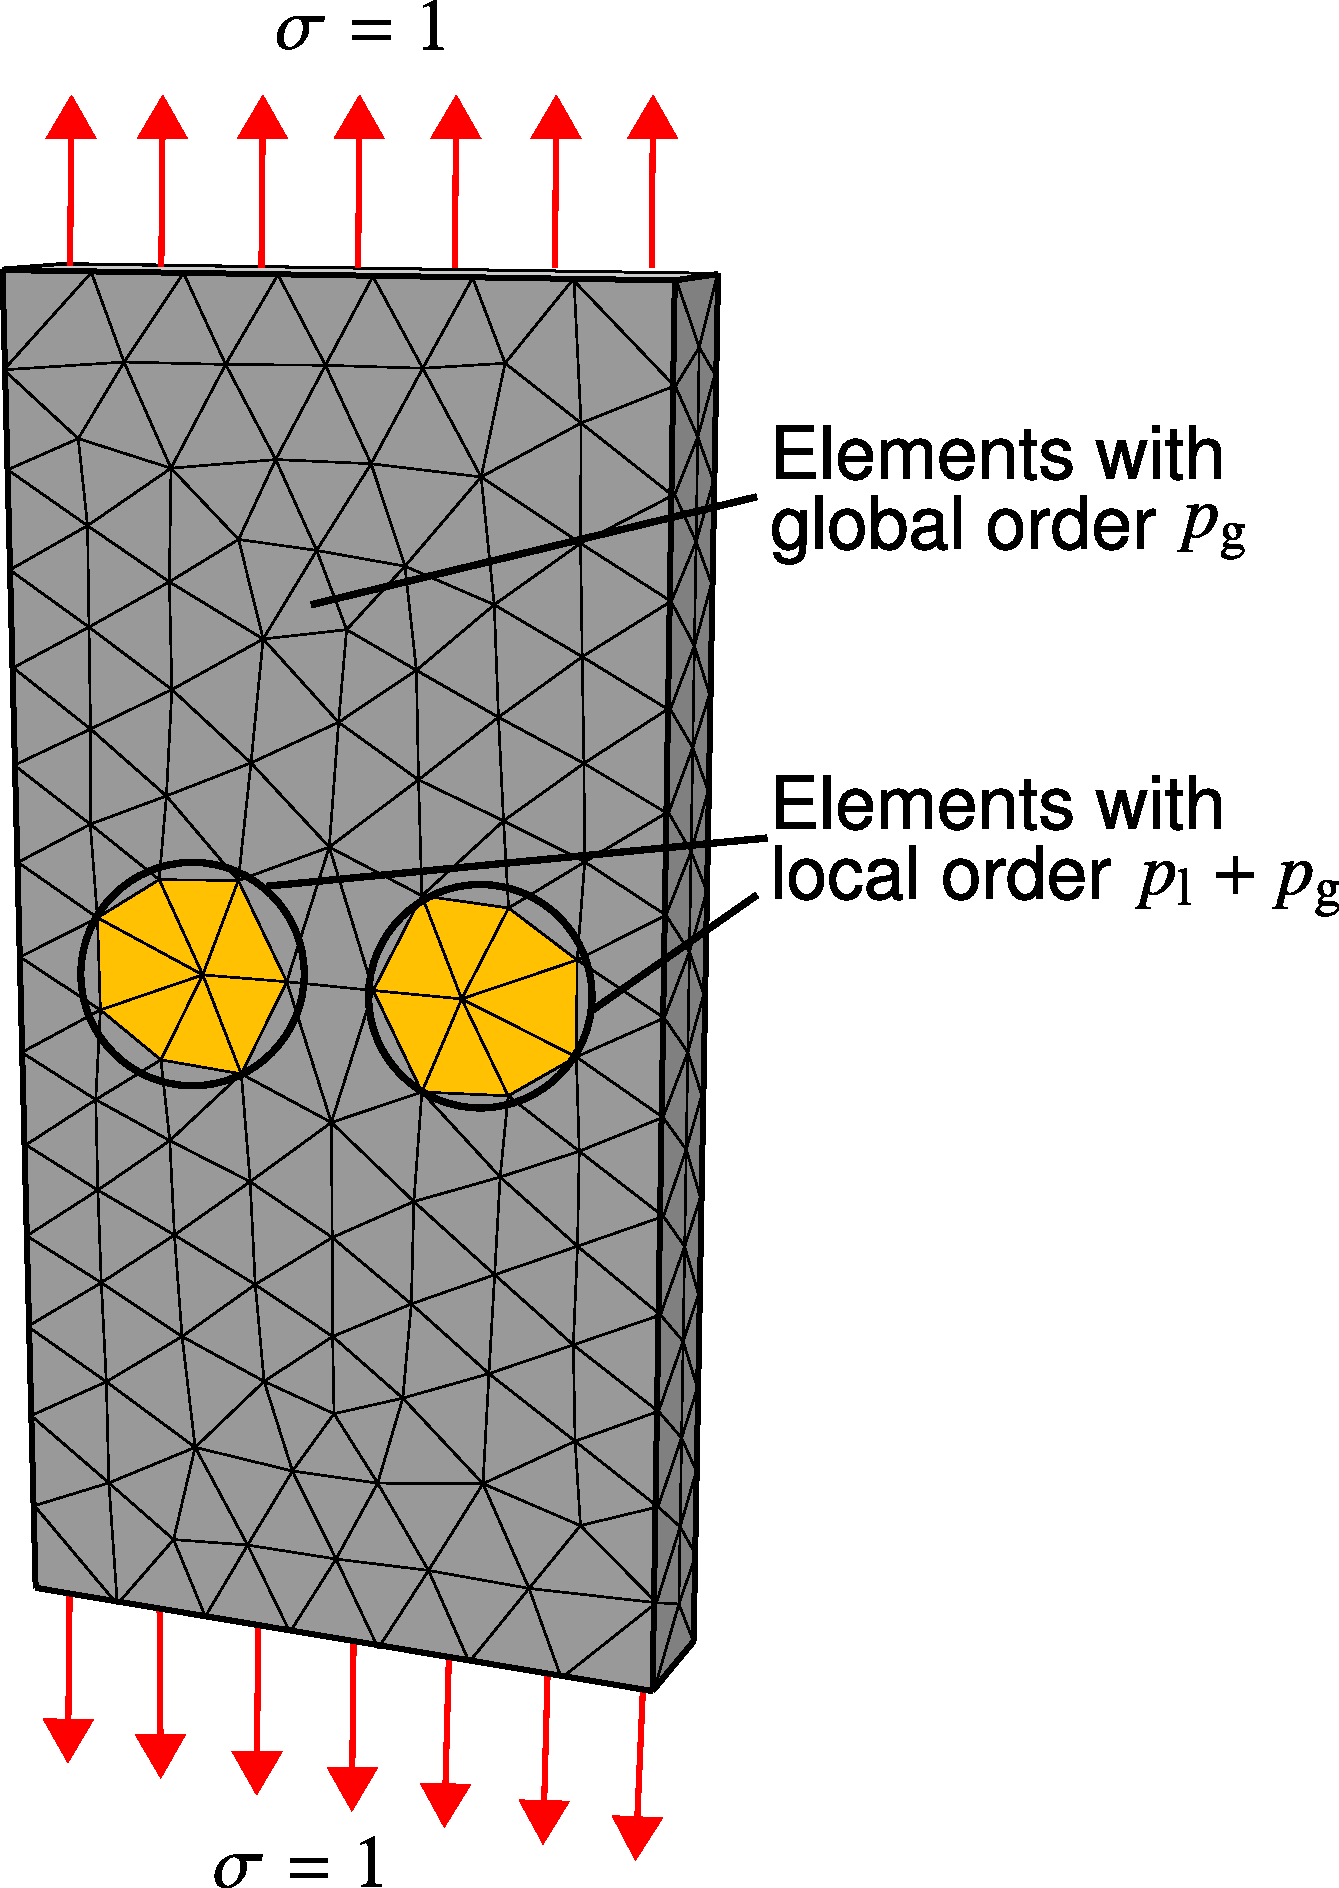
\includegraphics[height=8.5cm]{Figures/InfSlabMeshs.pdf}}\\  
(a) & &  & (b) 
\end{tabular}
\caption{Finite plate with a horizontal crack. a) Dimensions of specimen and through thickness crack. b) Applied uniaxial stress $\sigma$ and finite element mesh for $p_{\rm l} + p_{\rm g} \leq 3$ where elements presented with gray colour have approximation order $p_{\rm g}$ and elements that have vertices at crack tip, presented with yellow colour, have approximation order $p_{\rm l}+p_{\rm g}$.}
\label{fig:plate_load_mesh}
\end{center}
\end{figure}

The purpose of this analysis is to calculate the Mode I stress intensity factor $ K_{\rm I} $ and compare the results to the following analytical solution~\citep{rooke1976compendium} for infinite plate:
\begin{equation}\label{eq:frac_analytical}
K_{\rm I}=\sigma \sqrt{\pi a_{\rm {pl}}} \left[  \frac{1 - \frac{a_{\rm {pl}}}{2b_{\rm {pl}}} + 0.326 (\frac{a_{\rm {pl}}}{b_{\rm {pl}}})^2 }{\sqrt{1-\frac{a_{\rm {pl}}}{b_{\rm {pl}}}}}  \right]
\end{equation}
where $\sigma $ is the applied stress. 
%Dimensions of the specimen are presented in Figure~\ref{fig:plate_load_mesh} along with the finite element model consisting of 1384 tetrahedral elements. 
Young's modulus $E$ and Poisson's ratio $\nu$ are $1000$ and $0.3$, respectively. 


Hierarchical approximation basis functions allows for usage of elements with different orders of approximation. 
Hence, the influence of local and global $p$~-~refinement is investigated.
In general, all tetrahedrons of the mesh have a global order of approximation, $p_{\rm g}$, and the elements that are subjected to local refinement have order from $p_{\rm{l}} + 1$~to~$p_{\rm{l}} + p_{\rm{g}}$.
When $p_{\rm l}+p_{\rm g}\leq3$, two types of tetrahedral elements are considered where local order of approximation is increased to $p_{\rm l}+p_{\rm g}$ only at elements with vertices at the crack tip as presented in Figure~\ref{fig:plate_load_mesh}b.
Otherwise, a number of groups of tetrahedrals with different orders of approximation are considered.
Similar to the case where $p_{\rm l} + p_{\rm g} \leq 3$, the first group of elements is composed of the tetrahedrals with vertices at the crack tip and have approximation order $p_{\rm l}+p_{\rm g}$.
The second group of elements is consisted of the tetrahedrons adjacent to the first set elements, with approximation order that is one less than the previous set, i.e. $p_{\rm l}+p_{\rm g}-1$.
This process continues for each next adjacent group of tetrahedrons until the approximation order reaches the global order of approximation, $p_{\rm {g}}$.

All analyses presented were run using the same mesh for 1st order up to 6th order of approximation with local $p$~-~refinements so that $p_{\rm l} + p_{\rm g} \leq 7$, since this is the current limitation of implemented quadrature rule. 
The Mode I stress intensity factor, $K_{\rm I}$, can be calculated directly from the output material forces using the following relationship: 
\begin{equation}
K_{\rm I} = \sqrt{GE}
\end{equation}
where $G$ is the change of elastic strain energy per unit area of crack growth.
The deformed shape of the plate is illustrated in Figure~\ref{fig:plate_conv_no_sing}.
From the graph, it is evident that for the same coarse mesh and number of nodes the solution can improve drastically when the order of approximation is increased. 
The well known pathological nature of the 1st order solution due to shear locking is observed since a much higher error than other orders is computed. 
The minimum achieved error is $0.6\%$ for all the cases with total order of approximation  $p_{\rm l} + p_{\rm g} = 7$. 
Therefore, it can be observed that the same level of accuracy can be accomplished when using a low order of global approximation with only local $p$~-~refinement as with high order on the entire mesh. 
Moreover, by looking at the number of degrees of freedom, it can be observed that using higher order elements locally results to the same accuracy at a much lower cost of computation time since the global matrix has a much lower size.
\begin{figure}
	\centering
	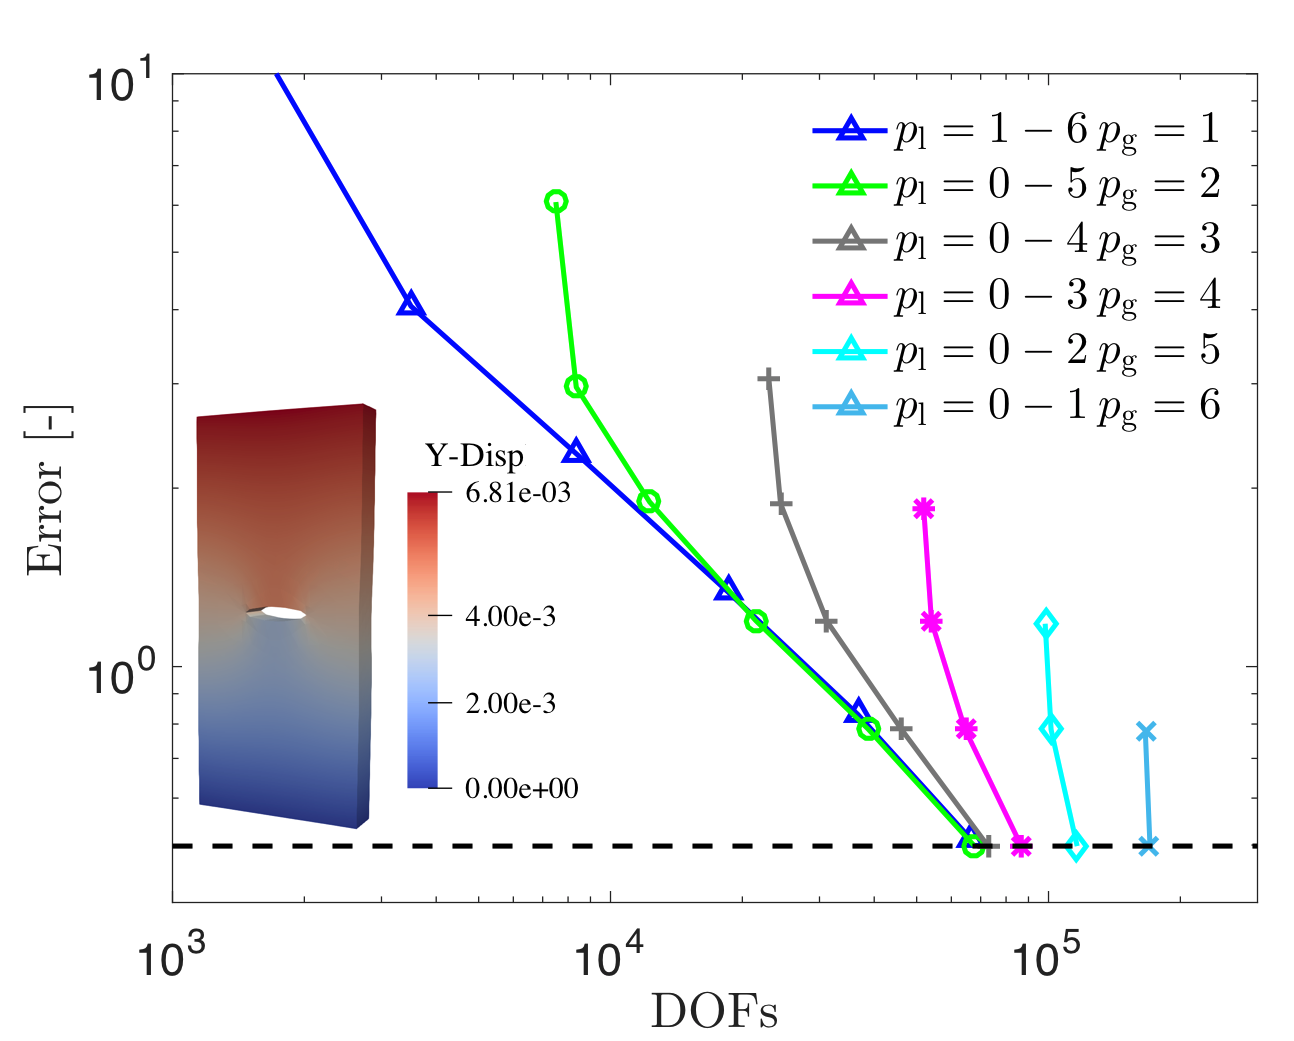
\includegraphics[width=0.7\linewidth]{Figures/graphs/plate_conv_no_sing.png}
	\caption{Convergence plot for stress intensity factor $K_{\rm I}$ Error (\%) versus no. of DOF (log10) and deformed shape of the plate (bottom left).}
	\label{fig:plate_conv_no_sing}
\end{figure}

%The use of finite element method to analyse fracture problems is complicated for many reasons. 
%One of them is stress field singularity located at the crack tip.
Conventional finite elements are interpolated by polynomials which are not able to reproduce infinite stresses at the crack tip. 
In the mid-1970s, two independent contributors~\citep{barsoum1976use,henshell1975crack} showed that, the singularity at the crack tip can be modelled by considering shifting the mid-node of all edges connected to crack tip nodes.
The new mid-node position is at a quarter of edge length distance from the crack tip node known as the quarter-point position and the resulting element is known as quarter-point element. 
This results in a nonlinear mapping between natural (isoparametric) and local coordinates $\xi \rightarrow x$ which produces the singularity. 
%Ignatios: it is too early to use radius r_q this will be used later Stress and strain fields are dependent on the radial function of the crack tip, reaching infinity as $ r_{\rm q} \rightarrow 0$. \\

The concept of quarter point element is briefly described by means of 1D 2-nd order finite element with standard base shape functions. 
Global configuration of 2-nd order element with nodes 0, 2 and 1 is schematically presented in Figure~\ref{fig:1d-quarter}(a) where node 0 coincides with the crack tip.
Furthermore, the natural coordinate system of the element is presented in Figure~\ref{fig:1d-quarter}b and the corresponding standard shape functions $N_0$, $N_2$ and $N_1$ are presented in Figure~\ref{fig:1d-quarter}c.  
Let the demonstrated element be a quarter-point type, the distance between node 0 with nodes 2 and 1 is given by radial coordinate $r_{\rm q}$ (see Figure~\ref{fig:1d-quarter}(a)). 
The position of the middle node 2 is controlled by the parameter $\kappa$. 
The quadratic 1D displacement function of this element is: 
\begin{equation}\label{eq:crack_disp_func}
\begin{aligned}
&u(\xi) = \sum_{a=0}^2 N_a (\xi) u^{(a)} = \frac{1}{2} \xi (\xi - 1)u^{(0)} + (1 - \xi^2)u^{(2)} + \frac{1}{2} \xi (\xi + 1)u^{(1)} =\\
& u^{(2)} + \frac{1}{2}(u^{(1)} - u^{(0)})\xi + \left[ \frac{1}{2} (u^{(0)} + u^{(1)}) - u^{(2)} \right] \xi^2 
\end{aligned}
\end{equation}

\subsubsection{Quarter point elements} %should that be in appendix?
\begin{figure}[h!]
\begin{center}
\begin{tabular}{c c c c}
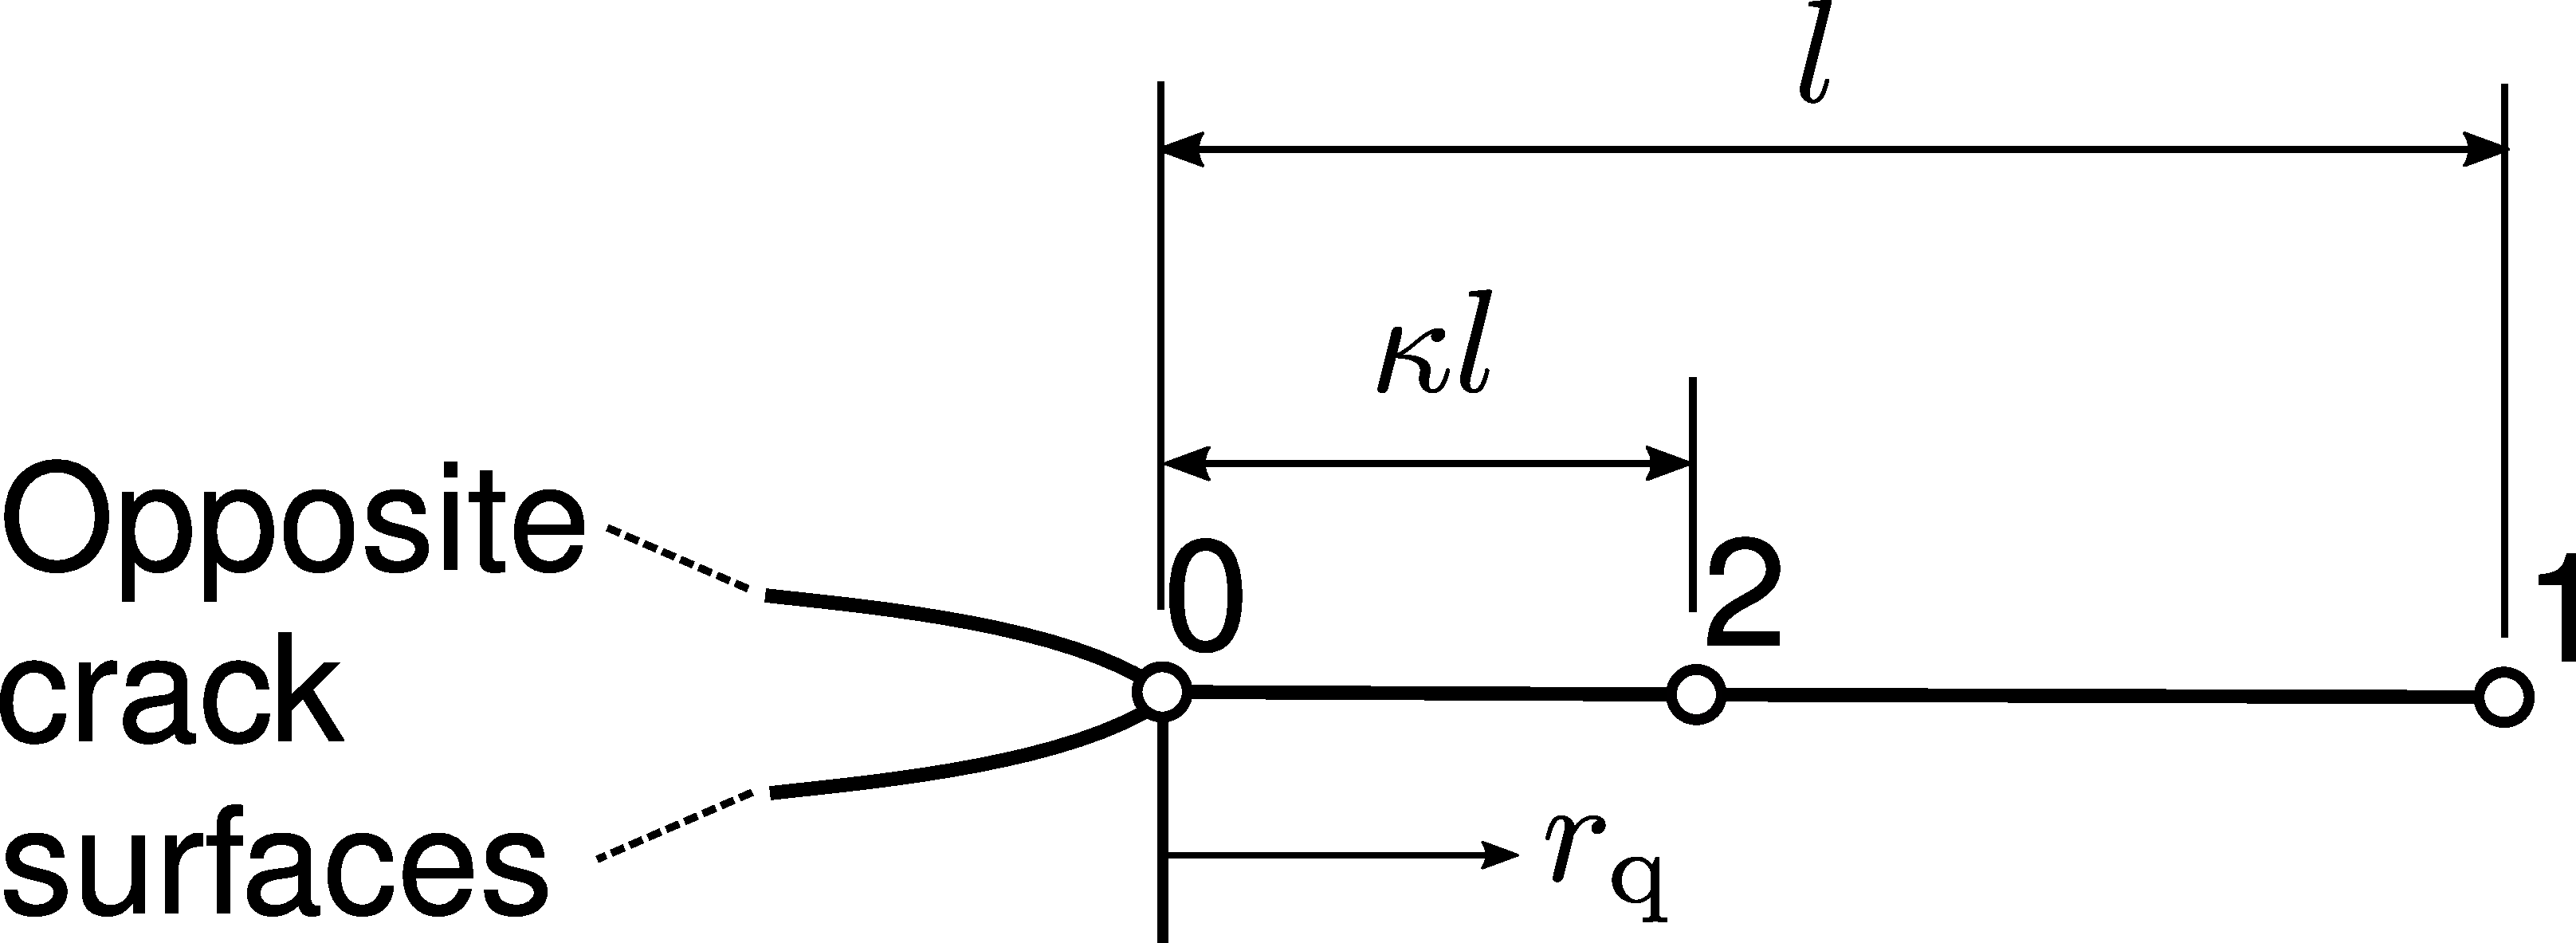
\includegraphics[height=2.cm]{Figures/QuarterPoint.pdf}  & 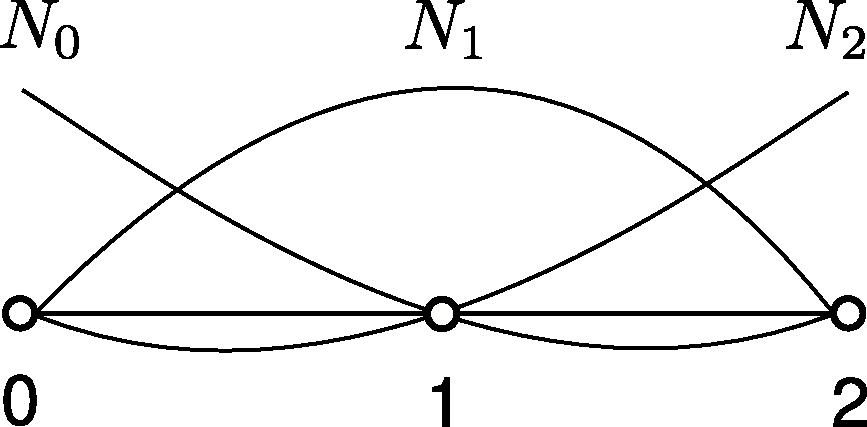
\includegraphics[height=2.1cm]{Figures/2ndOrderNodeOr.pdf} &   &  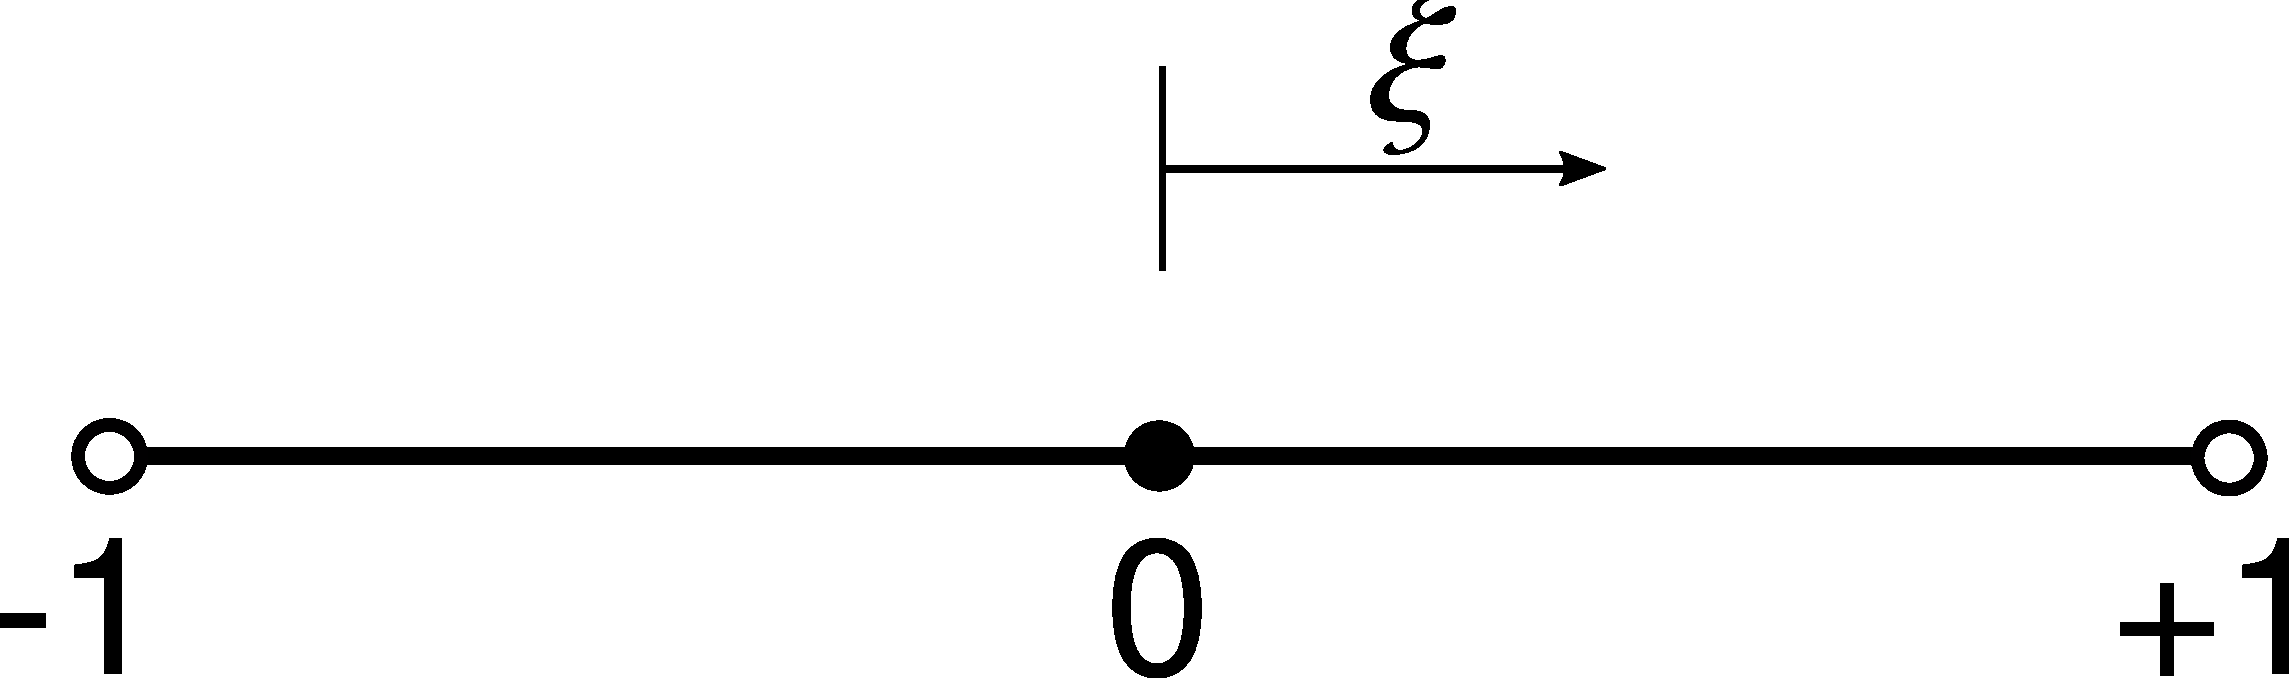
\includegraphics[height=1.3cm]{Figures/StandardElement.pdf}\\  
 (a) & (b)& &(c)
\end{tabular}
\caption{1D 2-nd order quarter-point element with standard shape functions:a) global configuration, b) natural coordinates, c) base shape functions }
\label{fig:1d-quarter}
\end{center}
\end{figure}

Note that Eq.~(\ref{eq:crack_disp_func}) is ordered by powers of $\xi$ that is element natural coordinate. 
In the classical isoparametric formulation, the same interpolation functions are also used for the coordinates, i.e. as well for the radius $r_{\rm q}$ with the nodal values $r^{(0)}_{\rm q} = 0$, $r^{(2)}_{\rm q} = \kappa l$, $r^{(1)}_{\rm q} = l$:
\begin{equation}\label{eq:crack_radius_dep}
r_{\rm q}(\xi) = \sum_{a=0}^2 N_a (\xi) r^{(a)}_{\rm q} = \kappa l + \frac{1}{2} l \xi  + \left(  \frac{1}{2} - \kappa \right) l \xi^2.
\end{equation}
Any value chosen for $\kappa$ would fulfil equality $r_{\rm q}(\xi=-1) = 0$ in Eq.~(\ref{eq:crack_radius_dep}).
However, the aim of quarter point element is to generate an approximated displacement field, $u(r_{\rm q})$, so that the resulting strains evaluated as $\varepsilon (r_{\rm q}) = \partial u(r_{\rm q})/\partial r_{\rm q}$.
To achieve this, a $r^{\theta}_{\rm q}$ term with $\theta < 1$ in Eq.~(\ref{eq:crack_disp_func}) should be pursued.
Here, value $\kappa = 1/4$ is used providing the following relations:
%From Eq.~(\ref{eq:crack_radius_dep}) it can be derived that radius $r_{\rm q}(\xi=-1) = 0$ for $ \kappa=1/4$, providing the following relations:
\begin{equation}
r_{\rm q}= \frac{l}{4}(1+\xi)^2 \quad \Rightarrow \quad \xi = 2 \sqrt{\frac{r_{\rm q}}{l}} -1,
\end{equation}
which substituted into Eq.~(\ref{eq:crack_disp_func}) results to an expression with a term $r^{0.5}_{\rm q}= \sqrt{r_{\rm q}}$ renders the desired radial dependence of the displacements $u(r_{\rm q})$ and strains $\varepsilon(r_{\rm q})$:
\begin{equation}
\begin{aligned}
u(r_{\rm q}) = u^{(0)} &+ \left( -3u^{(0)} - u^{(1)} +4u^{(2)} \right) \sqrt{\frac{r_{\rm q}}{l}} + 2 \left( u^{(0)} + u^{(1)} -2 u^{(2)} \right) \frac{r_{\rm q}}{l}\\
\varepsilon(r_{\rm q}) = \frac{\partial u}{ \partial r_{\rm q}} = &+ \left( - \frac{3}{2}u^{(0)} - \frac{1}{2}u^{(1)} +2u^{(2)} \right) \frac{1}{\sqrt{lr_{\rm q}}} + 2 \left( u^{(0)} + u^{(1)} -2 u^{(2)} \right) \frac{1}{l}
\end{aligned}
\end{equation}
The displacement function contains now a constant (rigid body motion) and linear function also a $\sqrt r_{\rm q}$ term, which reproduces the displacement field at the crack tip. 
The strain in the quarter-point element possesses the square root $1/{\sqrt r_{\rm q}}$ singularity.
\subsubsection{Hierarchical shape functions}
In this subsection, the concept of 1D 2-nd order quarter-point element formulation with standard shape function is extended to the case of hierarchical shape functions.
It should be mentioned that quarter-point elements used in the present contribution are for 3D and arbitrary order.
Presentation of 1D/2-nd order is merely done to convey main element attributes, i.e. reproduction of infinite stresses at crack tip.
A more detailed description for higher dimensions can be found for example in~\citep{nejati2015use}.

Here, global configuration of quarter-point element presented in Figure~\ref{fig:shape_funcs}(a) is considered.
In hierarchical shape functions~\citep{Ainsworth2003} no extra nodes are added for functions of order higher than the first one therefore the element under considerations is consisted of two nodes (0 and 1 in Figure~\ref{fig:shape_funcs}a)). 
%The hierarchical shape functions' values for an arbitrary high-order shape function are created in a hierarchical algorithm. 
This feature greatly simplifies $p$~- and $hp$~- adaptivity implementation.
Moreover, natural coordinate system and hierarchical shape functions $N_0$, $N_1$ and $N_2$ are presented in Figure~\ref{fig:shape_funcs}b and Figure~\ref{fig:shape_funcs}c, respectively.

Since $u^{(2)}$ degree of freedom associated to the 2-nd order shape functions $N_2$ is not related to a physical node, fictitious location of the degree of freedom can be achieved through multiplication of shape function with coefficient $\kappa$. 
Therefore, Eq.~(\ref{eq:crack_disp_func}) can be written for hierarchical shape functions as:

\begin{figure}[h!]
\begin{center}
\begin{tabular}{c c c c}
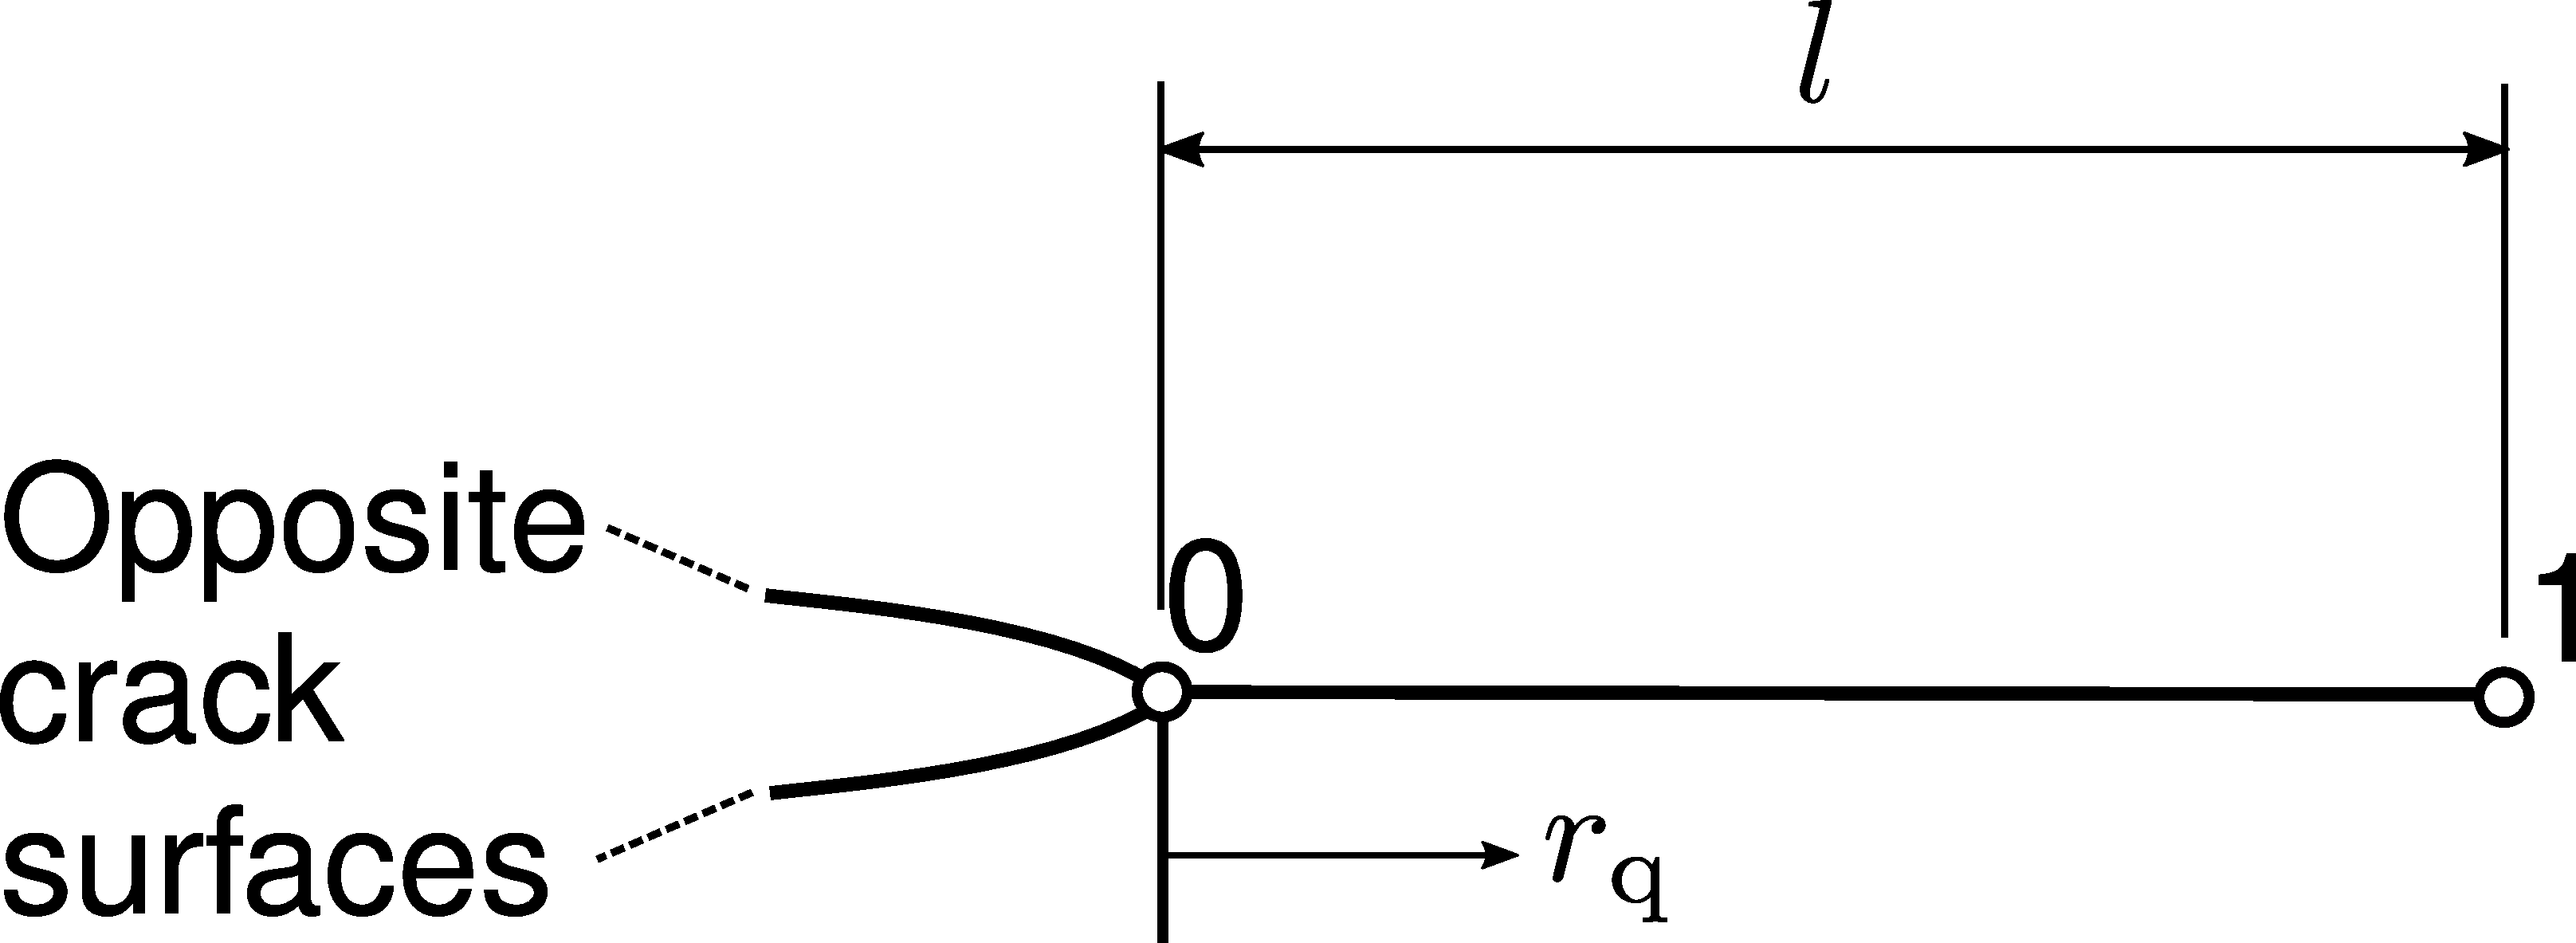
\includegraphics[height=2.cm]{Figures/QuarterPointHierarchical.pdf}  & {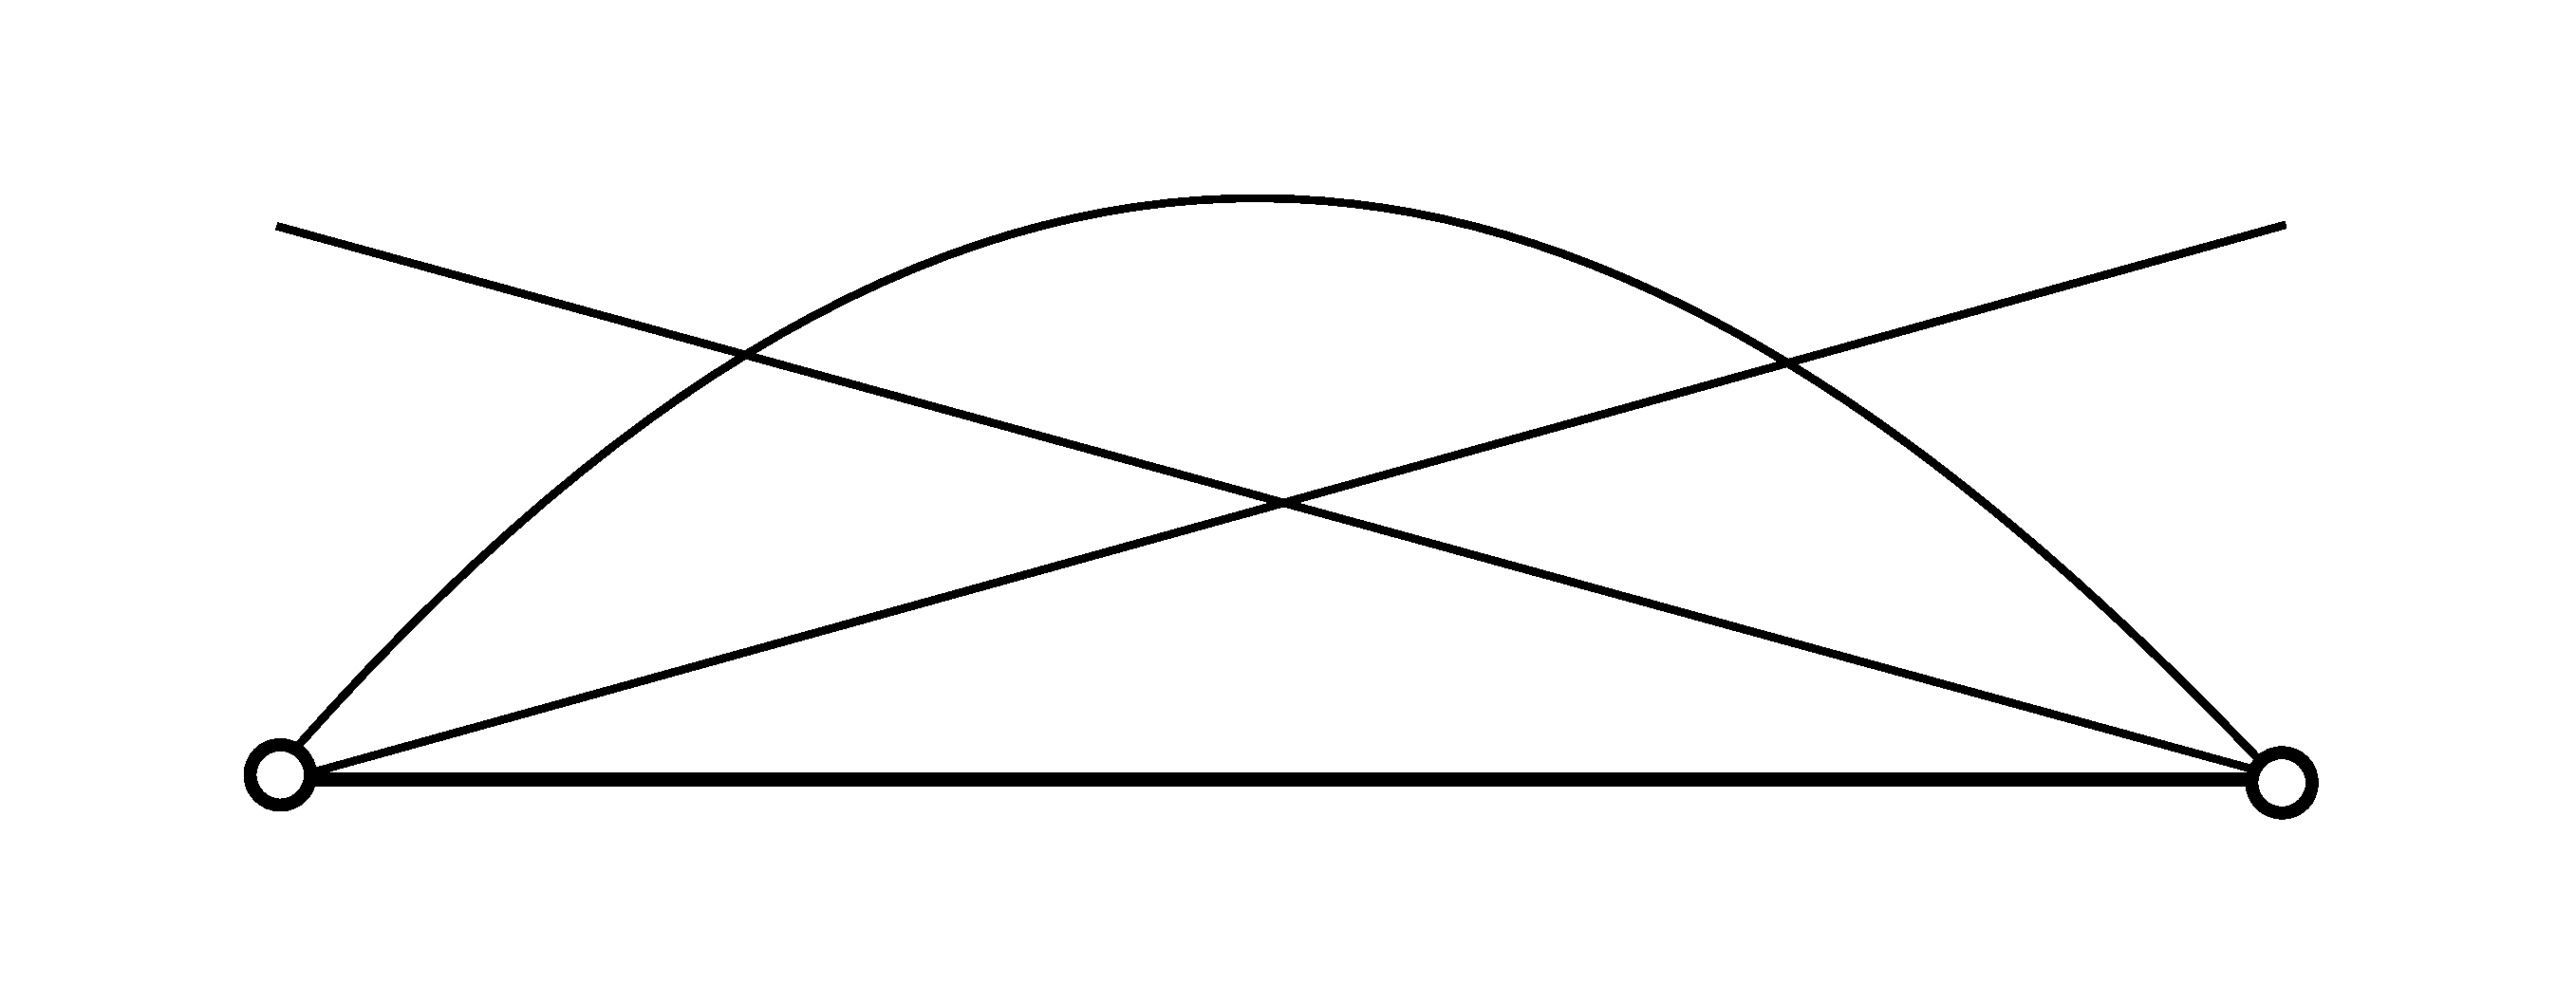
\includegraphics[height=2.cm]{Figures/Hierarchical2nd.pdf}} & &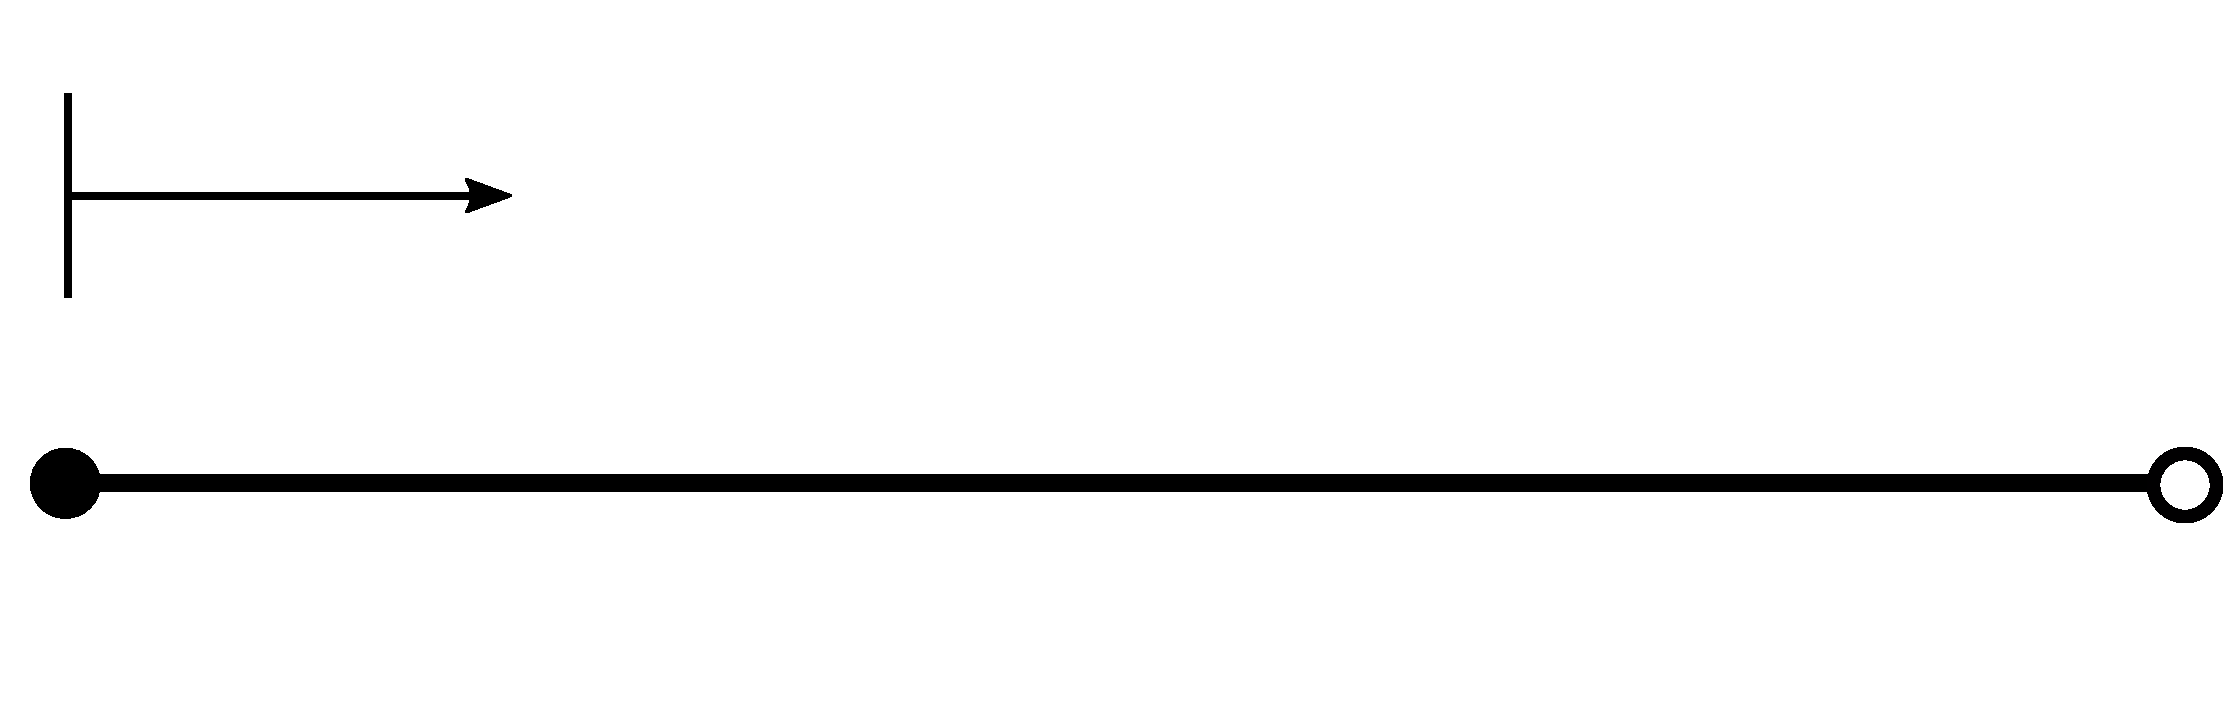
\includegraphics[height=1.3cm]{Figures/HierarchicalNaturals.pdf}\\  
 (a) & (b) & & (c)\\  
\end{tabular}
\caption{1D 2-nd order quarter-point element with hierarchical shape functions: a) global configuration b) natural coordinates, c) base shape functions.}
\label{fig:shape_funcs}
\end{center}
\end{figure}


\begin{equation}\label{eq:hierarchical_u}
u(\xi) = \sum_{a=0}^2 N_a (\xi) u^{(a)} = (1 -\xi)u^{(0)} + \xi(1 - \xi)u^{(2)}\kappa + \xi u^{(1)}
\end{equation}
Rewriting the above Eq.~(Eq.~(\ref{eq:hierarchical_u})) in terms of the radius $r$ takes the form:
\begin{equation}\label{eq:hierarchical_r}
r_{\rm q}(\xi) = \sum_{a=0}^2 N_a (\xi) r^{(a)} = \xi l + \xi(1-\xi)  l  \kappa
\end{equation}
To achieve generation of a $\sqrt{r_{\rm q}}$ term in Eq.~(\ref{eq:hierarchical_u}) by substitution of $\xi$ by an expression of $r_{\rm q}$, $\kappa = -1$ is chosen and solving Eq.~(\ref{eq:hierarchical_r}) results to relation:
\begin{equation}
r_{\rm q}= \xi l - \xi(1-\xi)l \quad \Rightarrow \quad \xi = \sqrt{\frac{r_{\rm q}}{l}},
\end{equation}
which yields the following radial dependence for displacements and strains:
\begin{equation}\label{eq:singstrain}
\begin{aligned}
u(r_{\rm q}) &= u^{(0)} + \left( -u^{(0)} + u^{(1)} - u^{(2)} \right) \sqrt \frac{r_{\rm q}}{l} - u^{(2)} \frac{r_{\rm q}}{l}\\
\varepsilon(r_{\rm q}) &= \frac{\partial u}{\partial r_{\rm q}} = \left( u^{(0)}  + u^{(1)} - u^{(2)}  \right) \frac{1}{2} \sqrt \frac{l}{r_{\rm q}} + u^{(2)} \frac{1}{l}
\end{aligned}
\end{equation}
Expressions in Eq.~(\ref{eq:singstrain}) have the necessary terms to reproduce rigid body motion and pass the patch tests, as well as the desired $1 / \sqrt r_{\rm q}$ singularity.
This should enable the elements adjacent to the crack front to reproduce strain singularity resulting in a more accurate finite element solution~\citep{nejati2015use}. 
The influence of the similar procedure with tetrahedral elements will be investigated in the following section.
\subsubsection{Convergence with quarter-point elements}
Here, results of the convergence upon $p$~-~refinement will be presented with the same problem as demonstrated in Section~\ref{sec:plate_section}. 
This time, however, quarter-point tetrahedral elements were applied around the crack front.
\begin{figure}[h!]
	\centering
	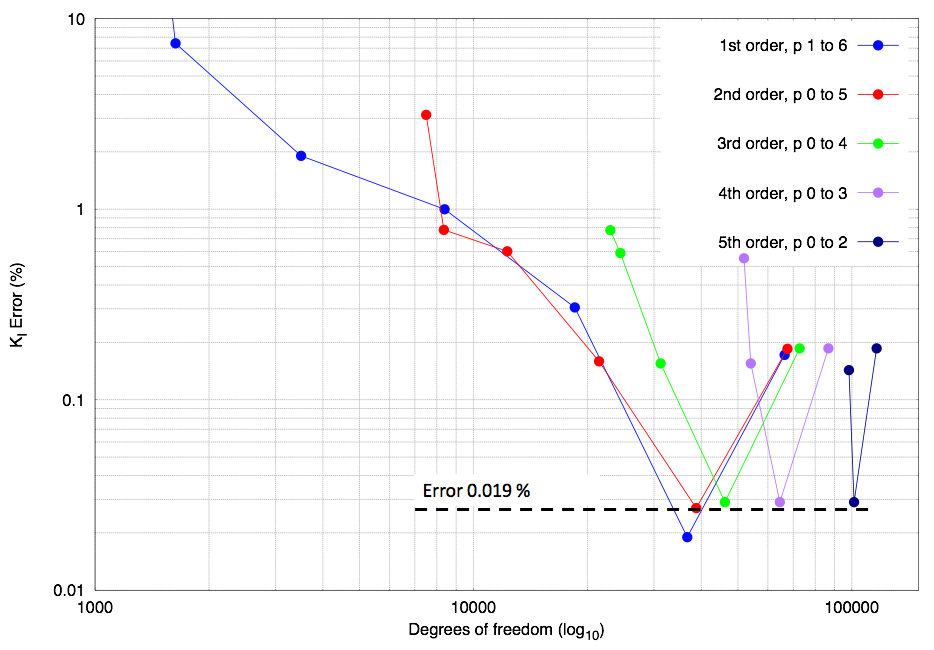
\includegraphics[width=0.7\linewidth]{Figures/graphs/plate_conv_singularity.png}
	\caption{Convergence plot for stress intensity factor $K_{\rm I}$ Error (\%) versus no. of DOF (log10).}
	\label{fig:plate_conv_singularity}
\end{figure}
Based on the results in Figure~\ref{fig:plate_conv_singularity}, it is evident that using quarter-point elements improves the convergence rate to the analytical solution significantly. 
Introducing the singularity at the crack tip elements lowered the error by an order of magnitude, from 0.636\% down to 0.02\%. 
However, it can be seen from the plot in Figure~\ref{fig:plate_conv_singularity} that for each $p_{\rm l} + p_{\rm g}$ case, just after reaching the minimum error, it starts increasing up to a certain value. 
This suggests that the solution cannot be further improved beyond that point only by enhancing the order of approximation. 
Possibly, by refining the mesh and changing model dimensions (since an analytical solution is for infinite plate), the error could be decreased even more. 
Nevertheless, such accuracy is redundant for engineering purposes. \\
%The critical thickness is that which causes the specimen to be dominated by a state of plane strain, as opposed to plane stress. The stress in the through-thickness z direction must become zero at the sides of the specimen since no traction is applied there, and in a thin specimen the stress will not have room to rise to appreciable values within the material. The strain in the z direction is not zero, of course, and the specimen will experience a Poisson contraction given by εz = ν(σx + σy). But when the specimen is thicker, material near the center will be unable to contract laterally due to the constraint of adjacent material. Now the z-direction strain is zero, so a tensile stress will arise as the material tries to contract but is prevented from doing so. 
Overall, these results indicate that it is of great benefit to use quarter-point elements, since they improve the accuracy of the solution with no extra cost.
Furthermore, the difference in execution time for the analysis with and without their inclusion was negligible. 
\subsubsection{Validation of material forces in the heterogeneous body}
So far, this article has focused on cracks in homogeneous bodies. 
The following subsections will discuss the influence of including inhomogeneities into the domain. 
Considering the same problem of the finite plate with horizontal crack, as in the previous analyses, a density field $\mathbf{\rho}(x,y,z) = 0.125y + 1$ is directly assigned at integration (Gauss) points of each tetrahedral element.
Once again, stretching the specimen introduces some material forces at the crack tip and also on the entire domain due to inhomogeneity. 
Since the stress intensity factor loses its meaning in the case of heterogeneous bodies, correct validation of material forces still remains an open question. 
To the best of the authors' knowledge, the current state of literature lacks in numerical methods to verify the results of material forces or stress intensity factors for heterogeneous solids other than functionally graded materials~\citep{kim2002finite}.
%, by using MLS method, demonstrated in Section~\ref{sec:mwls}.

It was decided that a straightforward verification can be performed by using simple numerical differentiation method like centered Finite Difference Method (FDM). Following Griffith's work~\citep{Griffith163}, the release energy rate for crack growth can be calculated as the change in elastic strain energy per unit area of crack growth:
\begin{equation}
G = \frac{\partial \psi}{\partial a_{\rm {pl}}}
\end{equation}
where $\psi$ is the elastic energy of the system, and $a_{\rm{pl}}$ is the crack length. Moving on, this derivative can be calculated by aforementioned FDM as follows:
\begin{equation}
 \frac{\partial \psi}{\partial a_{\rm {pl}}} = \lim_{\Delta a_{\rm {pl}} \to 0} \frac{\psi(a_{\rm {pl}} + \Delta a_{\rm {pl}}) - \psi(a_{\rm {pl}} -\Delta a_{\rm {pl}})}{2\Delta a_{\rm {pl}}}
\end{equation}
where the elastic strain energies $\psi(a_{\rm {pl}} \pm \Delta a_{\rm {pl}})$ can be obtained simply by running two additional analyses of the finite plate with horizontal cracks of lengths: ($a + \Delta a_{\rm {pl}}$) and ($a - \Delta a_{\rm {pl}}$), where $\Delta a_{\rm {pl}}$ is a very small value. 
Next, knowing the resulting release energy with the crack length of $a_{\rm {pl}}$, an elative error can be calculated. 
Twenty-six sets of three analyses (for different $p$~-~refinements) have been performed in order to determine the error in the release energy. 
The results are presented in Figure~\ref{fig:covergencefdm}.
\begin{figure}
	\centering
	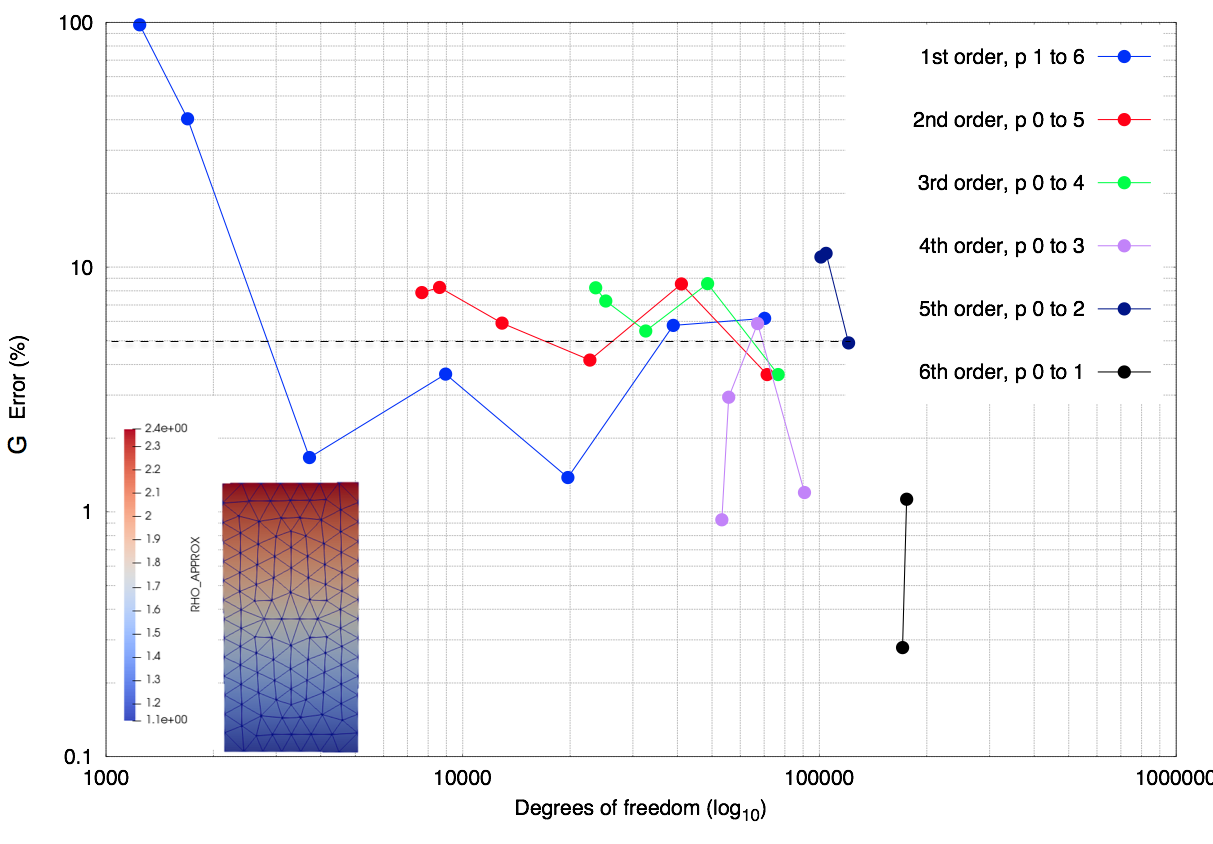
\includegraphics[width=0.7\linewidth]{Figures/graphs/covergence_FDM.png}
	\caption{Convergence of error in release energy rate from Finite Difference Method. Density distribution (bottom left).}
	\label{fig:covergencefdm}
\end{figure}
It is apparent from this plot that for most of the refinements the error in release energy is less than 5\%.
Therefore, it can be deduced that the presented implementation allows for estimation of release energy for heterogeneous domains with a satisfactory level of accuracy.
\subsubsection{Release energy rate for metacarpal bone from CT}
This numerical example considers the same bone as presented in Section~\ref{sec:numerical_examples:bone_adap}. 
The generated mesh with an initial crack is shown in Figure~\ref{fig:bone_ct_mesh_cut} and consists of 6069 tetrahedral elements. 
The notch is situated at the origin of the most common location of lateral condyle fracture~\citep{jacklin2012frequency}. 
The numerical analyses were undertaken using three meshes consisted of 6069, 10032 and 21189 tetrahedrons and repeated for 1st, 2-nd and 3rd-order of local $p$~-~refinement at the crack tip. 
Boundary conditions and material parameters remain the same as in Table~\ref{tab:parameters_mc3}. 
Using a $ \mathrm {K_2 HPO_4  }$ calibration phantom, gray scale values from CT are converted to bone mineral density using five tubes with reference densities. 
The mechanical material properties were mapped onto the integration points of the metacarpal mesh using the MLS method described earlier. 
Applying load onto the bone surface introduces some material forces in the entire domain, with the highest values at the singularity i.e notch tip. 
Resulting nodal material forces are illustrated in Figure~\ref{fig:crackfrontforce}. 
The direction of the vectors also indicates the direction of crack propagation.
%When these forces, attain the critical value, crack growth is spontaneous and catastrophic.  
The values of numerically predicted maximal nodal release energy rates in Mode I (crack opening) for subsequent meshes are plotted in Figure~\ref{fig:max_g1_convergece}. 
It can be seen that, for the same mesh, as approximation order increases material forces reach a plateau. 
%with increasing order of approximation material forces converge.
\begin{figure}
	\centering
	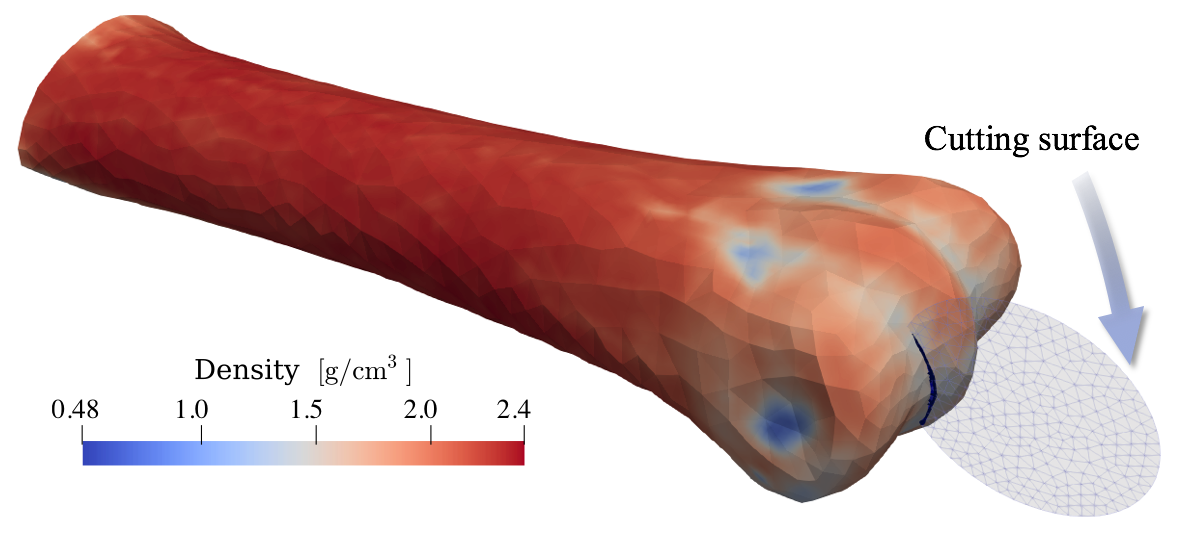
\includegraphics[width=0.5\linewidth]{Figures/bone_ct_mesh_cut.png}
	\caption{Bone geometry with mapped density from CT by using MLS. In order to calculate the material forces, an initial crack is introduced by cutting the mesh with a circular surface. The cutting algorithm is not limited to planar cracks. }
	\label{fig:bone_ct_mesh_cut}
\end{figure}

\begin{figure}
	\centering
	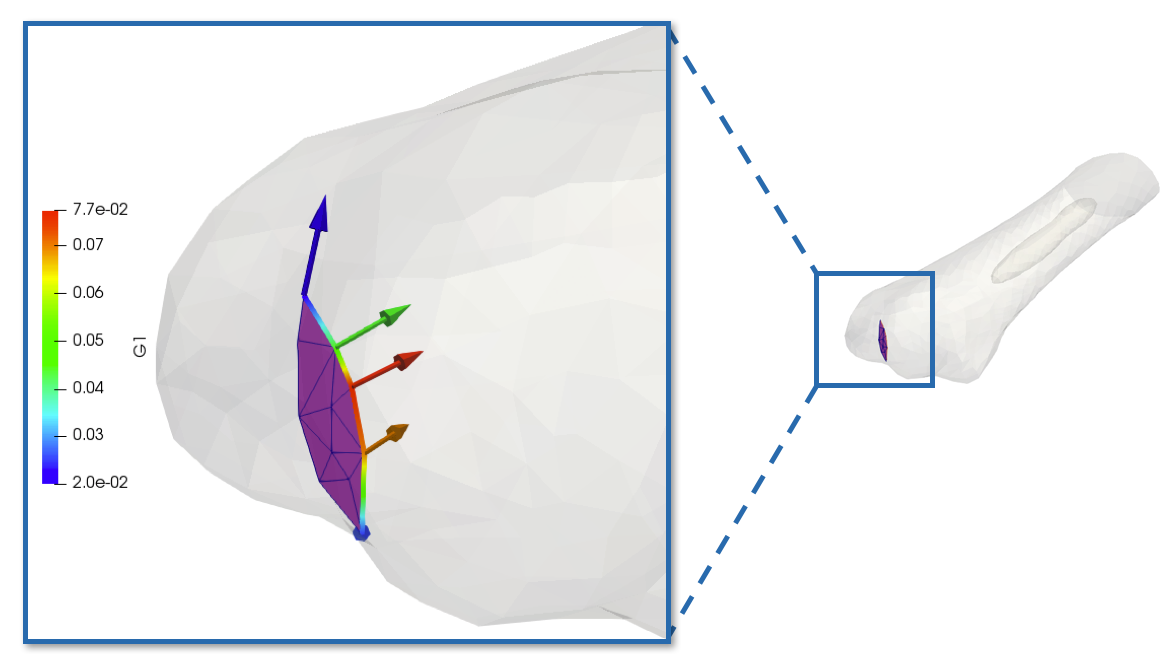
\includegraphics[width=0.9\linewidth]{Figures/crack_front_force.png}
	\caption{Crack surface and vectors of material (crack driving) forces at the front.}
	\label{fig:crackfrontforce}
\end{figure}

\begin{figure}
	\centering
	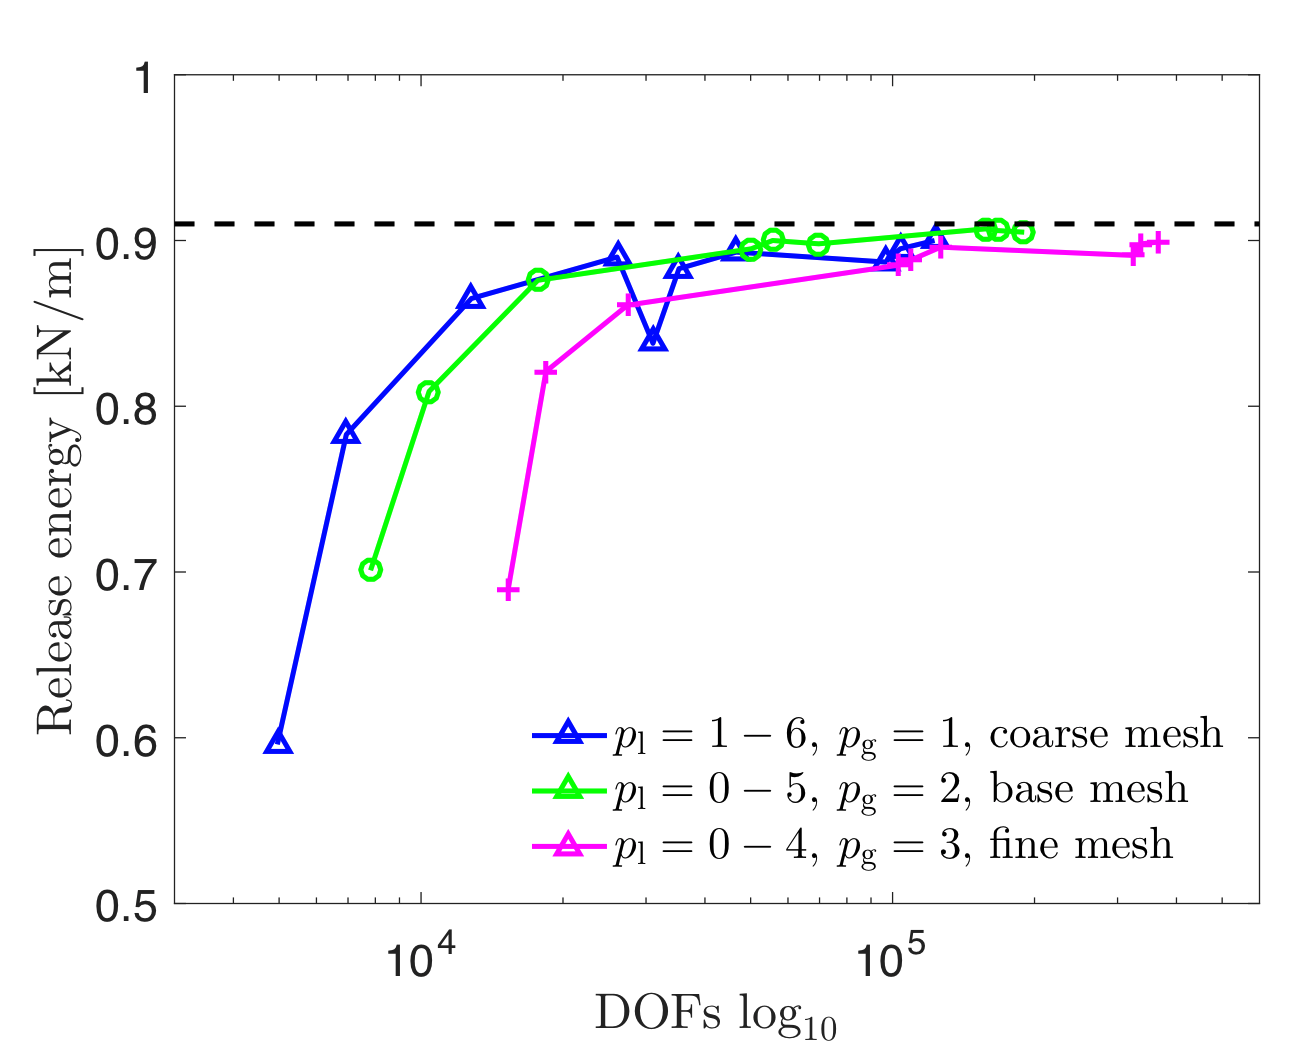
\includegraphics[width=0.7\linewidth]{Figures/graphs/max_g1_convergece.png}
	\caption{Convergence plot of maximum material force in Mode-I versus no of DOF (log10) for subsequent discretisations and $p$~-~refinements. Results are mesh independent since they all converge to the value for release energy of approximately $ G_{\rm I} = 0.9 \, [\mathrm{kJ} / \mathrm{m}^2]$ for increasing approximation order. }
	\label{fig:max_g1_convergece}
\end{figure}
Crack extension occurs when the energy release rate $G$ equals the material's resistance, $g_{\rm c}$ to crack extension. 
Assuming that bone's resistance is $g_{\rm c} = 2.0\,[\mathrm{ kJ/m^2}]$ )~\citep{gasser2007numerical} it can be estimated that this particular metacarpal can sustain loading of approximately 2.2 times greater before fracture starts to propagate. 
\subsubsection{Release energy rate for remodelled bone}
The numerical example described in this section presents an application of the developed framework to estimate the crack propensity of the equine metacarpal bone at different phases of adaptation during training. 
The same geometry and boundary conditions as in the previous example are used here. 
However, this time, densities from bone adaptation (Section~\ref{sec:numerical_examples:bone_adap}) are mapped on a mesh consisting of 6069 elements as demonstrated in Figure~\ref{fig:frackmeshcutting}. 
\begin{figure}
	\centering
	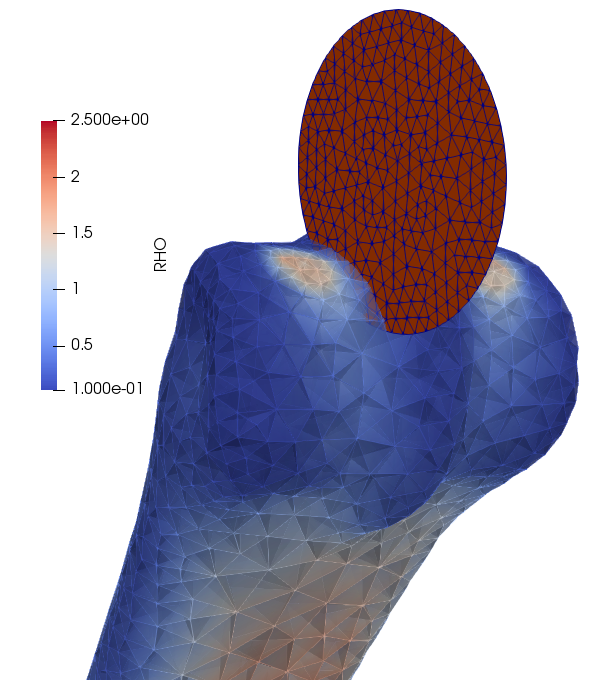
\includegraphics[width=0.8\linewidth]{Figures/frack_mesh_cutting.png}
	\caption{Cut in the mesh of the remodelled 3rd metacarpal bone. The resulting density from the bone adaptation analysis is approximated directly onto integration points of the new model by using MLS method described earlier in Section~\ref{sec:mwls}. }
	\label{fig:frackmeshcutting}
\end{figure}
The resulting energy rate at different points in time of bone adaptation are illustrated in Figure~\ref{fig:crackmc3release} for three different local $p$~-~refinements. The difference between analysis with increased order at the crack tip is very small. 
\begin{figure}
	\centering
	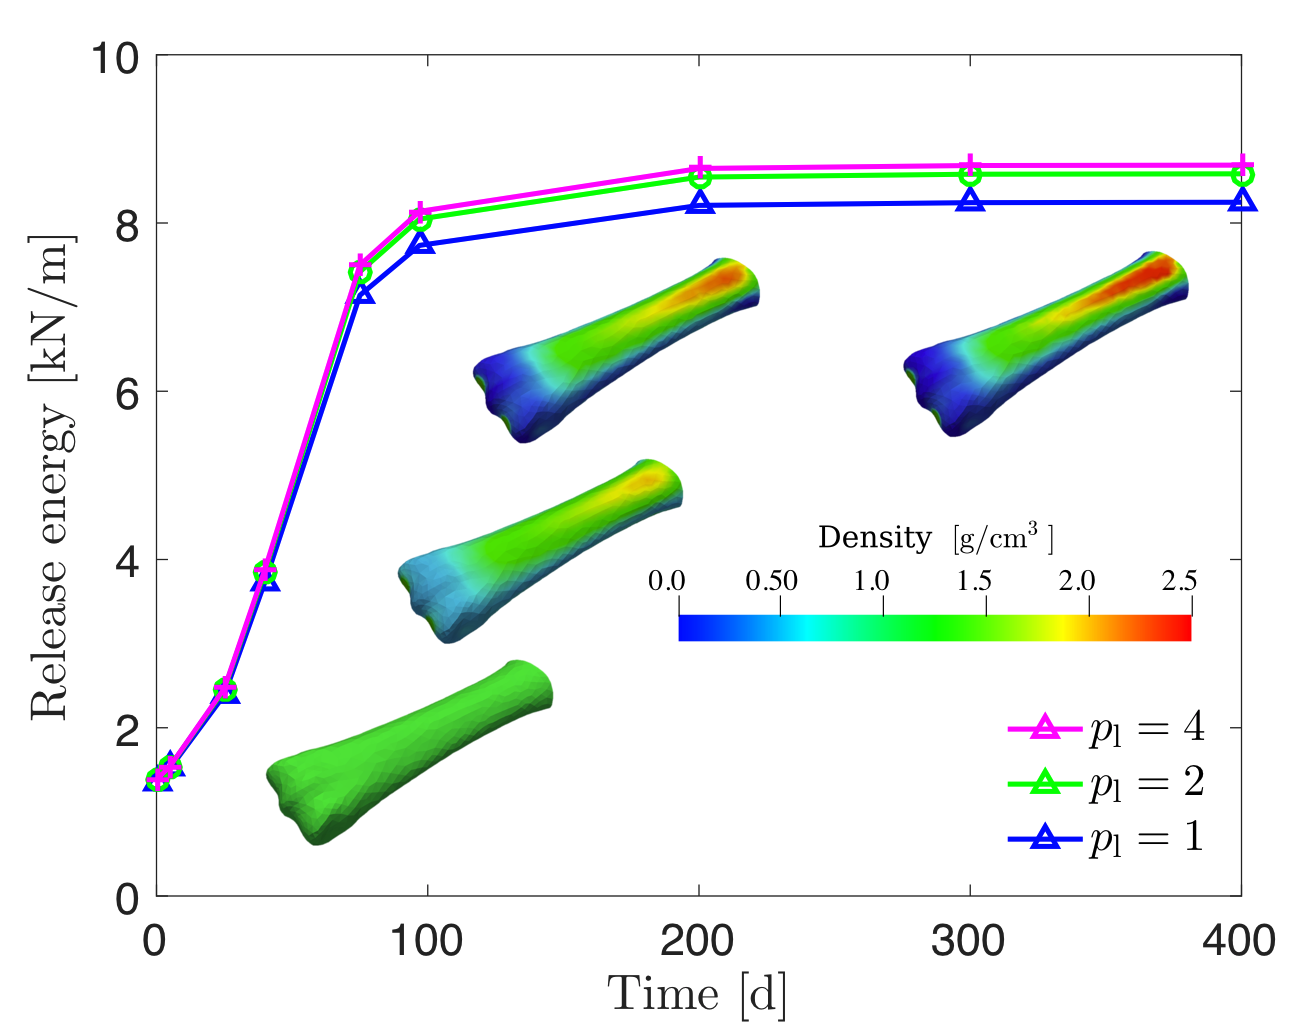
\includegraphics[width=1\linewidth]{Figures/graphs/crack_mc3_release.png}
	\caption{Material forces for remodelled bones for three local $p$~-~refinements.}
	\label{fig:crackmc3release}
\end{figure}
The numerical outcomes clearly capture the general trend of increasing release energy rate over time for racehorses' bones. It can be seen that by introducing a notch in the resorption zone, where no loading is applied, the material force attains larger values. This indicates that over time the presented bone becomes more prone to fracture in the specific region. 


%SIMPLY: energy release per unit length of a crack advancement has to be equal energy consumption for the creation of the new surface in the circuital conditions and its equal to %material parameter - fracture energy. Griffith theory
%$-\frac{\partial \psi}{\partial a} = \frac{\partial S}{\partial a} = \mathcal\mathbf G_c$

\section{Discussion}\label{sec:discussion}
Development of a 3D Finite Element model for biological applications is a very complicated process. 
Unlike that in typical engineering research subjects, there is still very little knowledge of the material properties. 
Another issue is lack of proper definition of the boundary conditions. Constraints are mostly explicit when analysing engineering objects such as concrete beams or steel frames under different loading conditions. 
However, in a living body it is challenging to accurately define loads. 
Model geometry suffers from inaccuracies in scanning as well as segmentation process. 
Results from such models could potentially include an increasing number of errors since the data collected from each stage of the 
model creation encompasses high ancertenty data~\citep{campoli2014effects}.
Available information is usually subject-specific or gathered for a relatively small population of subjects and cannot be generalised. 
Subsequently, even if one manages to overcome the aforementioned obstacles, there is a need for validation of such models, which will also have to deal with similar difficulties. 
%A possible number of errors increase at each stage of creating such models since there is high uncertainty about obtained data~\citep{campoli2014effects}. 

Over the years, many frameworks have been developed to quantify such uncertainty levels, which might greatly increase the credibility of computational models~\citep{wille2016uncertainty}. 
CT scanning on living horses limbs is still too cumbersome to be used as a standard diagnostic tool.
As to best authors' knowledge there is a limited number of facilities that can perform CT scanning for horses without the necessity for anaesthesia. 
Nevertheless, this study can bring new insight in the area of catastrophic injuries in order to improve the welfare of the thoroughbred racehorse. %The successful application of developed framework would enable the introduction of interventions for veterinary practitioners, such as suggestions for training regimes based on known risk factors for lateral condylar fractures that could reduce the probability of fracture in racehorses. \\

In summary, the goals of this study were to: (i) implement bone remodelling algorithm to predict density levels in response to high-intensity training for racehorses, (ii) to incorporate an efficient and accurate mapping strategy to represent heterogeneous bone material properties for hierarchical finite element models and (iii) to assess the potential of linear fracture mechanics in evaluating bones' propensity to failure. 
Despite certain limitations, it was demonstrated that the implemented open systems thermodynamics framework allows for simulation of a natural behaviour of hard biological tissues. 
The proposed computational method may have a great potential to identify the risk of fracture related to changes in bone mineral density. 
Understanding the effects of changing release energy in response to bone remodelling can help developing training regimes that reduces the liability of fatal injury. 
Furthermore, the model uses very few parameters which can be experimentally determined in a practical manner increasing the attractiveness of this approach.\\ 

Application of a bell function to enforce bounds on density levels in the constitutive model did not provide rigid constrains for density levels, but merely slowed down the convergence to the biological equilibrium process. 
Nevertheless, it may still become useful, when one tries to fit the model parameters into the actual density data form CT scanning in defined periods of time. 
One could also constrain density bounds by introducing and calibrating mass influx to the balance of mass equation~\citep{sharma2013adaptive}. 
Nonetheless, bones in the living organisms are never fully load adapted~\citep{christen2014bone}. 
Therefore, achieving a biological equilibrium that results in unrealistic levels of density should never take place in a real case scenario. \\

This contribution also investigated the application of a meshless MLS method in approximating the density data on FE models. Validation of analytical field mapped on a simple mesh and comparison with LS method on mapping data from CT scanning was conducted and proved that MLS can be a suitable technique for the approximation of density field, even with strong gradients. 
Nevertheless, the accuracy of the presented approach still has to be validated experimentally, for example, in the prediction of strains in the loaded bone specimen.  \\

A novel method in quantifying bone fracture propensity was presented. By scanning the bone, running the bone adaptation simulation and subsequently introducing a notch in the geometry at particular time steps, it can be observed from the values of material forces how loading the bone influences its resistance to fracture. 
This framework, can be potentially a very useful tool in diagnostic of fractures and eventually prevention of catastrophic failures. 
Moreover, the code used for all numerical analyses was developed keeping in mind scalability and robustness. 
Entire framework can be executed on parallel computer system in order to fit in an efficient patient-specific modelling routine that can handle many patients within a practical time window. \\

Numerical examples demonstrated the accuracy of the proposed framework. 
Convergence has been validated for all examples, in particular, the use of quarter point elements was shown to improve the convergence of calculated release energy rates. 
\subsection{Limitations and future work}
The methods presented in this paper have several important limitations. 
Considerably more work has to be done to determine bone loading, since using simplified input results in unrealistically low densities in non load-bearing regions. 
Multiple load cases can be critical in modelling bone adaptation~\citep{geraldes2016consideration}. 
In the future, the forces will be obtained by using gait data and musculoskeletal analysis~\citep{Delp2007} combined with FEM mortar contact formulation in MoFEM~\citep{athanasiadis2018mortar}. 
Another method to predict realistic loading is to solve an~inverse problem to bone remodelling. 
Promising results have been reported in that field by using machine learning methods like Neural Networks~\citep{campoli2012computational}. 
The current linear fracture mechanics approach does not take into account nonlinear cohesive mechanisms like collagen fiber bridging at the crack tip~\citep{yang2006fracture}. 
Therefore, the calculated release energy with presented approach might be overestimated. 
More research is also required to calibrate material parameters, in particular those regarding constitutive relations for bone remodelling. 


%Overall, the presented examples of density evolution, at this point are not sufficient to make any practical conclusions about the remodelling of the metacarpal bones. \\


%Calculation of release energy rate does not give any insights into quantitative strength of the bones' structure. Future implantation on an implicit crack propagation for heterogeneous bodies will allow to trace a full dissipative loading path. The process of determining detailed musculoskeletal loads using kinematic data and external forces is called inverse dynamic analysis

%Another limitation of the study is that only one load case is considered. 
%However, it is important to note that while simulating bone functional adaptation a detailed knowledge of the actual loading situation is elementary. By assuming that all three cases occur simultaneously in some loading conditions forces could balance each other.

%The model is not yet calibrated and validated against patient data, however, it provides valuable insight to the bone remodelling behaviour for equine metacarpal and is capable of qualitatively comparing different loading.

%bone remodelling is not purely load-driven. Possible causes for this could be that also other mechanisms, for example, calcium homeostasis, influence normal bone remodelling and thus bone is never fully load adapted. as suggested in~\citep{christen2014bone}. The authors of previously mentioned publication also suggests that approximately 50\% of the bone structure might be determined by mechanical loading.


%No previous study has investigated release energy of brittle fracture in heterogeneous bodies like bones. 
%In the future we might use a micro CT scanning as ot was shown that it is currently the most accurate method to estimate bone strength. 
%We are hoping that when we refine the model we could confirm that bone remodelling may increase the propensity to cracks and find potential practical applications in the fracture prevention.
% this research can be easily translated into human applications 
%Presented framework could be also combined with other risk factors~\citep{georgopoulos2017risk} which should improve the clinical assessment of fracture risk
%The correlation between bone adaptation, high intense training and stress fractures is still poorly understood. The promising results of this study offer a novel framework to simulate  changes in the bone structure as a result of loading and quantify the risk of fatal injury. 
%In conclusion, this study has shown that fracture resistance in the equine metacarpal bone can be numerically quantified. 
%Understanding the effects of changing release energy in response to bone remodelling will help in the development of training regimes that reduces the risk of fatal injury in racehorses
%This approach might become especially handy to analyse whether a discovered crack in the equine bone is liable to propagate under certain loading conditions. 
%model with the capability to simulate the bone density growth and resorption processes due to mechanical stimuli
%A reduction in this specific type of fracture would have a significant global impact on the number of Thoroughb redracehorses subjected to euthanasia as a result of in jury incurred duringracing
%has a massive welfare and economic impact on horse racing

%A better understanding of the influence of race training on subchondral bone remodelling is essential to understanding the pathophysiology of subchondral bone injury.

%Therefore, the development of computational tools with the capability to estimate bone adaptation when prosthetic devices are used has a remarkable importance, since these processes may contribute to implant success or failure. In this scenario, the finite-element method (FEM) has been playing a key role, being used to study and evaluate the mechanical behaviour of prosthetic devices

%The flexibility of the hierarchic finite element is fully utilised, which permits the use of arbitrary order of approximation leading to accurate results for relatively coarse meshes. The developed computational framework is implemented in our group's FE software, MoFEM (Mesh-Oriented Finite Element Method). \\

%Moreover, the application of the study proposes a computational assessment tool for veterinary specialists, focused on the simulation of a healthy femur and a femur with an implanted prosthesis submitted to loads.

%The main objective advocated in this contribution is the setting up of a modelling framework relying on the thermodynamics of irreversible processes




\newpage
\bibliographystyle{abbrv}
\bibliography{bibfile}
\end{document}